%%%%%%%%%%%%% Partie obligatoire du préambule
\documentclass[a4paper,12pt,twoside]{book}
\usepackage{fontspec}
\usepackage{xunicode}
\usepackage[french]{babel}

%%%%%%%%%%%%%%%%%%%%%%%%%%%%%%%%% PACKAGES UTILISÉS

\usepackage{csquotes} % les guillemets français
\usepackage{lettrine} % faire une lettrine (pas obligatoire)

% Chargement du package biblatex
\usepackage[style=enc,sorting=nyt,maxbibnames=10]{biblatex} % charger le style de l'EnC
\addbibresource{bibliographie/jumeauNumérique.bib}
\addbibresource{bibliographie/ExemplesJN.bib}
\addbibresource{bibliographie/gestionDesDonnées.bib}
\addbibresource{bibliographie/Modélisation.bib}
\addbibresource{bibliographie/Divers.bib}
\nocite{*}
\defbibnote{intro}{Cette bibliographie présente toutes les ressources utilisées, de tout type, citées ou non, par simple ordre alphabétique.}

%%%%%%%%%%%%%%%%%%%%%%%%%%%%%%%%% AJOUT DE PACKAGE
\usepackage{graphicx} % Pour les insertions d'images
\usepackage{adjustbox} % Pour adapter la taille des images
\usepackage{lscape}
\usepackage{float}
\usepackage{tabularx} % Package pour un tableau ajustable
%\usepackage{tocbibind} % pour l'inclusion de la liste des figures etc à la table des matière


%%%%%%%%%%%%%%%%%%%%%%%%%%%%%%%%% CONFIGURATION DE MISE EN PAGE

%%%%%% Les compteurs (sections, subsections, etc)
\renewcommand{\thesection}{\Roman{section}.}%On ne fait apparaître que le numéro de la section
\renewcommand{\thesubsection}{\arabic{subsection}.}%subsection en chiffres arabes
\renewcommand{\thesubsubsection}{\alph{subsubsection}.}%subsubsection en lettres minuscules
%Si l'on veut faire apparaître les subsubsection dans le table des matières (à commenter sinon)
\setcounter{tocdepth}{3}

%%%%%% Mise en page École des chartes
\usepackage[margin=2.5cm]{geometry}
\usepackage{setspace}
\onehalfspacing % interligne de 1.5
\setlength\parindent{1cm}

% Pour retirer le titre courant d'une page vide avant un chapitre
\newcommand{\clearemptydoublepage}{\newpage{\pagestyle{empty}\cleardoublepage}}

%%%%% Mise en forme des headers (haut de page)
\usepackage{fancyhdr} % package utilisé pour modifier les headers
\pagestyle{fancy} % utiliser ses propres choix de mise en page et non ceux par défaut du package

\setlength\headheight{16pt} % la hauteur des headers
\renewcommand{\sectionmark}[1]{\markright{\small\textit{\thesection~\  #1}}} % Faire apparaître dans les headers les sections en petit et en italiques
\renewcommand{\chaptermark}[1]{\markboth{\small\chaptername~\thechapter~--\ \textit{#1}}} % idem pour les chapitres

% Package hyperref
\usepackage[xetex]{hyperref} % Inclure hyperref une seule fois
\hypersetup{
    pdfauthor = {Prénom Nom},
    pdftitle = {Titre du Document},
    pdfsubject = {Mémoire HN},
    pdfkeywords = {gestion des données, jumeau numérique, avion, patrimoine}, % Séparer les mots-clés par des virgules
    colorlinks = false, % Pour que les liens n'aient pas de couleur
    breaklinks = true, % Permet aux liens d'être sur plusieurs lignes
}

% Package bookmark, à mettre après hyperref
\usepackage[numbered]{bookmark} % Les signets seront numérotés


%%%%%%%%% GLOSSAIRE
\usepackage[toc=true]{glossaries}%doit être appelé après hyperref 
%(exception à la règle)
\makeglossaries

\newglossaryentry{foucault}{
    name={Analyse par courant de foucault},
    description={: L'analyse par courant de Foucault est une méthode qui utilise des courants électriques pour détecter des défauts à l'intérieur des matériaux sans les abîmer. Cette technique fonctionne comme une sorte de détecteur sophistiqué qui identifie des anomalies telles que des fissures ou des inclusions en mesurant comment les courants électriques se déplacent à travers le matériau. Lorsque le courant rencontre un défaut, il se comporte différemment, ce qui permet de localiser ces imperfections avec précision. Cette méthode est donc extrêmement utile pour inspecter des pièces ou des structures tout en préservant leur intégrité}
}

       \newglossaryentry{XRD}{
    name={Analyse par diffraction des rayons X},
    description={: Analyse la structure cristalline des matériaux pour identifier leur composition et leurs propriétés.La diffraction des rayons X (XRD) est une technique utilisée pour déterminer la structure cristalline des matériaux, autrement dit leur structure à l'échelle atomique. Le résultat de cette diffraction est un diffractogramme, un graphique qui montre l'intensité des rayons X diffractés en fonction de l'angle de diffraction et qui permet d'identifier la composition et les propriétés des matériaux en fournissant des informations sur la taille des cristallites, les phases présentes, et les déformations du réseau cristallin}
}

\newglossaryentry{EDS}{
    name={Analyses spectroscopiques EDS ou EDX},
    description={: Ces techniques utilisent des rayons X pour analyser les éléments d'un échantillon. Lorsqu'un échantillon est bombardé par des électrons, il émet des rayons X caractéristiques selon les éléments qui le constituent. En mesurant l'énergie de ces rayons X, on peut identifier les différents éléments présents dans le matériau. Cette technique permet de caractériser la composition élémentaire des matériaux}
}

\newglossaryentry{radionum}{
    name={Analyse par radiographie numérique},
    description={: La radiographie numérique est une technique d'examen qui utilise des rayons X pour créer des images détaillées de l'intérieur de structures et de matériaux, à l'image d'une sorte de radiographie moderne qui permet de voir ce qui se passe à l'intérieur sans avoir à ouvrir ou détruire l'objet examiné}
}

\newglossaryentry{Cloud}{
    name={Cloud},
    description={: Le Cloud Computing ou informatique en nuage est une infrastructure dans laquelle la puissance de calcul et le stockage sont gérés par des serveurs distants auxquels les usagers se connectent via une liaison Internet sécurisée}
}

\newglossaryentry{Endoscope}{
    name={Endoscope},
    description={: Cet outil permet de voir l'intérieur des zones difficiles d'accès en utilisant une petite caméra placée à l'extrémité d'un tube flexible. Il est couramment utilisé pour examiner les cavités et structures internes sans recourir à des méthodes invasives}
}

\newglossaryentry{LIBS}{
    name={LIBS},
    description={: Acronyme de Laser-Induced Breakdown Spectroscopy (Spectroscopie de Rupture Induite par Laser en français), cette méthode utilise un laser pour créer un petit éclat de plasma sur la surface de l'échantillon analysé. Ce plasma émet une lumière caractéristique des éléments présents dans l'échantillon. En analysant cette lumière (plus particulèrement ses émissions spectrales), on peut identifier les éléments chimiques et leur concentration. C'est une technique permettant de déterminer la composition chimique d'un matériau}
}

\newglossaryentry{Manipstat}{
    name={Manipulations potentiostatiques},
    description={: La manipulation potentiostatique est une technique en électrochimie où l'on maintient constant le voltage d'une électrode par rapport à une référence, tout en observant le courant généré. Cette méthode permet de mieux comprendre comment un matériau réagit à un certain voltage et de caractériser précisément les réactions électrochimiques, comme celles qui causent la corrosion, lorsque le voltage est fixe}
}

\newglossaryentry{Manipdyn}{
    name={Manipulations potentiodynamiques},
    description={: Cette méthode consiste à faire varier le voltage appliqué au métal de manière contrôlée, puis à mesurer le courant électrique qui en résulte. Cette méthode aide à voir comment la réactivité du métal change en fonction du voltage, et permet de comprendre comment il se corrode ou se protège dans différentes conditions}
}

\newglossaryentry{metado}{
    name={Métadonnées},
    description={Une métadonnée est une information descriptive qui apporte un éclairage supplémentaire sur une donnée principale. Elle agit comme une étiquette qui permet de mieux comprendre, organiser, et retrouver la donnée à laquelle elle se rapporte. Par exemple, dans le cas d'une photographie numérique, la métadonnée pourrait inclure des détails tels que la date de prise de vue, les paramètres de l'appareil photo, ou le lieu où la photo a été prise. C'est un outil de contextualisation qui enrichit la donnée brute, facilitant ainsi son utilisation et son exploitation.}
}

\newglossaryentry{MicroscopieBinoculaire}{
    name={Microscopie binoculaire},
    description={: Utilisée pour l'observation détaillée des échantillons à fort grossissement, cette technique a recours à un microscope possédant deux oculaires, ce qui lui permet une vision stéréoscopique et un meilleur confort pour l'utilisateur lors de l'examen de spécimens}
}

\newglossaryentry{MicroscopieOptique}{
    name={Microscopie optique},
    description={: Cette technique requiert un appareil qui utilise la lumière visible pour observer les échantillons. Il est largement utilisé pour examiner des spécimens translucides ou préparés sur des lames, permettant l'étude de structures à une échelle microscopique}
}

\newglossaryentry{MEB}{
    name={Microscope électronique à balayage},
    description={: Cette technique utilise un faisceau d'électrons (plutôt que la lumière visible) pour analyser les surfaces des échantillons à une résolution très élevée. Le microscope électronique à balayage permet d'obtenir des images détaillées de la topographie et de la composition des surfaces à un degré de précision plus élevé que celui d'un microscope optique}
}

\newglossaryentry{NAS}{
    name={Serveur de stockage en réseau},
    description={: Un serveur de stockage en réseau, également appelé stockage en réseau NAS, boîtier de stockage en réseau ou plus simplement NAS (de l'anglais Network Attached Storage), est un serveur de fichiers autonome, relié à un réseau, dont la principale fonction est le stockage de données en un volume centralisé pour des clients réseau hétérogènes}
}

\newglossaryentry{OUG}{
    name={Ondes ultrasonores guidées},
    description={: Une onde ultrasonore guidée est une technique avancée d’inspection non destructive qui utilise des ondes acoustiques pour détecter des défauts à l'intérieur des matériaux. Contrairement aux ondes ultrasonores ordinaires, qui se dispersent dans toutes les directions, les ondes guidées sont soigneusement orientées le long d'un trajet défini au sein du matériau. Ce contrôle précis de la propagation des ondes, réalisé à l'aide de méthodes spécialisées, permet d'obtenir une analyse plus détaillée et ciblée des structures examinées}
}

\newglossaryentry{SFX}{
    name={Spectrométrie à fluorescence X},
    description={: Cette technique permet de déterminer les éléments présents dans un échantillon. Lorsqu'un échantillon est exposé à des rayons X, il émet une fluorescence spécifique à chaque élément. En mesurant cette fluorescence, on peut ainsi identifier les éléments et leur concentration dans l'échantillon}
}

\newglossaryentry{Raman}{
    name={Spectrométrie RAMAN},
    description={: Cette technique permet d'identifier les molécules présentes dans un échantillon en étudiant la manière dont elles interagissent avec la lumière. Lorsqu'un laser éclaire un échantillon, la lumière est dispersée de manière spécifique par les molécules. En analysant les changements de fréquence de la lumière dispersée, on peut déterminer la structure et la composition moléculaire de l'échantillon}
}

\newglossaryentry{Table}{
    name={Table},
    description={: En modélisation relationnelle, une table est la structure qui stocke les données dans une base de données. Elle est composée de lignes et de colonnes. Chaque ligne représente un enregistrement (ou une instance) d'une entité, et chaque colonne représente un attribut (ou une caractéristique) de cette entité}
}

% COMMANDS
\renewcommand{\chaptermark}[1]{\markboth{\small\chaptername~\thechapter~--\ \textit{#1}}{}}

% Nouvelle commande pour les chapitres, qui permet d'avoir des titres d'en-tête plus courts, mais de garder les longs titres dans la table des matières

\newcommand{\chapwithshorttitle}[3]{%
  \chapter[#3]{#2}% #3 est utilisé pour la table des matières, #2 pour le corps du texte
  \markboth{#1}{#1}% #1 est utilisé pour les en-têtes (gauche et droite)
}

% Nouvelle commande pour les sections, , qui permet d'avoir des titres d'en-tête plus courts
\newcommand{\secwithshorttitle}[3]{%
  \section[#3]{#2}% #3 est utilisé pour la table des matières, #2 pour le corps du texte
  \markright{#1}% #1 est utilisé pour l'en-tête
}

% pour les remerciements, le résumé et l'introduction, afin qu'ils ne soient pas numérotés en tant que chapitre
\newcommand\mychapter[1]{%
  \chapter*{#1}%
  \markright{\MakeUppercase{#1}}% for the header
}

% Définir le style de page sans en-tête
\fancypagestyle{nohead}{
    \fancyhf{} % Efface tous les en-têtes et pieds de page
    \fancyfoot[C]{\thepage} % Numéros de page au centre du pied de page
}
% Définir une nouvelle commande pour appliquer le style sans en-tête
\newcommand{\noheads}{
    \pagestyle{nohead}
}

\title{Gestion et modélisation de la donnée en vue de la création d’un jumeau numérique d’avion}
\author{Prénom Nom - M2 TNAH}

%%%%%%% CORPS DU MÉMOIRE 

\begin{document}

\onehalfspacing 

\frontmatter

\begin{titlepage}
    \begin{center}
        \bigskip
        
        \begin{large}                
            ÉCOLE NATIONALE DES CHARTES\\
            UNIVERSITÉ PARIS, SCIENCES \& LETTRES
        \end{large}
        \begin{center}\rule{2cm}{0.02cm}\end{center}
        
        \bigskip
        \bigskip
        \bigskip
        \begin{Large}
            \textbf{Maddalena Accardo}\\
        \end{Large}
        
        \begin{normalsize} 
            \textit{licencié.e ès lettres}\\
            \textit{diplômé.e de master} 
        \end{normalsize}
        
        \bigskip
        \bigskip
        \bigskip
        
        \begin{Huge}
            \textbf{Jumeau numérique et patrimoine aéronautique : la gestion des données au coeur du projet C-ADER}\\
        \end{Huge}
        \bigskip
        \bigskip
        
        \vfill
        
        \begin{large}
            Mémoire 
            pour le diplôme de master \\
            \enquote{Technologies numériques appliquées à l'histoire} \\
            \bigskip
            2024
        \end{large}
    \end{center}
\end{titlepage}

\clearemptydoublepage

\frontmatter

\mychapter{Résumé}
\addcontentsline{toc}{chapter}{Résumé}
Ce mémoire a été réalisé à l’occasion d’un stage au Musée de l'Air et de l'Espace d'avril à juillet 2024, dans le cadre du Master « Technologies numériques appliquées à l’histoire » de l’École des chartes. Il explore le concept de jumeau numérique, un outil destiné ici, à la fin du projet C-ADER, à en valoriser les résultats et centraliser les données. Ce mémoire expose la nécessité de questionner et clarifier le concept de jumeau numérique. Cette clarification de ce que doit être l'outil final a pour but d'assurer une meilleure compréhension des données et de la manière dont elles doivent, à terme, être exploitées. En effet, le jumeau numérique est un outil de valorisation qui implique de centraliser, harmoniser, partager et stocker les données au sein d'un projet. Dans cette optique de gestion des données, une réflexion propre à la modélisation et à l'architecture des données en question a été menée.\\

This thesis was conducted during an internship at the Air and Space Museum from April to July 2024, as part of the Master’s program in ‘Digital Technologies Applied to History’ at the École des Chartes. It explores the concept of a digital twin, a tool intended here, at the conclusion of the C-ADER project, to enhance the outcomes and centralize the data. This thesis highlights the need to question and clarify the concept of a digital twin. The aim of clarifying what the final tool should be is to ensure a better understanding of the data and how it should ultimately be utilized. Indeed, the digital twin is a valorization tool that involves centralizing, harmonizing, sharing, and storing data within a project. In this context of data management, a specific reflection on the modeling and architecture of the data in question was carried out.\\

\textbf{Mots-clés:} gestion des données~; jumeau numérique~; numérique~; avion~; patrimoine.

\textbf{Informations bibliographiques:} Maddalena Accardo, \textit{Gestion et modélisation de la donnée en vue de la création d’un jumeau numérique d’avion}, mémoire de master \enquote{Technologies numériques appliquées à l'histoire}, dir. [Noms des directeurs.trices], École nationale des chartes, 2024.

\clearemptydoublepage

\mychapter{Remerciements}
\addcontentsline{toc}{chapter}{Remerciements}
\lettrine{M}es remerciements vont tout d'abord à toutes les personnes, enseignants comme élèves, qui m'ont accompagné tout au long de cette seconde année de Master. Je tiens également à remercier chaleureusement Agnès Mirambet-Paris, François Mirambet, Léa Ferfailles et Marine Zelverte, pour leur suivi tout au long de ce stage très enrichissant, et pour leurs précieux conseils. Je souhaite également adresser mes remerciements au personnel des secteurs Documentation et Conservation du Musée de l'Air et de l'Espace, et du département Archives et bibliothèques du C2RMF pour leur accueil. Enfin, je remercie très vivement Ségolène Albouy pour ses conseils et son accompagnement tout au long de cette expérience. 

\clearemptydoublepage

\printbibliography[keyword={jumeauNumérique},title={Jumeau numérique}]
\printbibliography[keyword={exemple},title={Exemples}]
\printbibliography[keyword={gestionDonnee},title={Gestion des données}]
\printbibliography[keyword={technique},title={Modélisation }]
\printbibliography[keyword={divers},title={Divers}]

\clearemptydoublepage

\mychapter{Introduction}
\addcontentsline{toc}{chapter}{Introduction}
\lettrine{L}{'}L'exposition temporaire intitulée « Antoine de St Exupéry, fragments d'histoires » inaugurée le 28 mai 2024 au Musée de l'Air et de l'Espace, rend hommage au pilote et écrivain Antoine de St Exupéry. Son objectif est double. Elle dévoile d'une part la diversité de la carrière aéronautique de St Exupéry ainsi que ses contributions littéraires. D'autre part, elle met en avant les techniques et sciences qui sont mobilisées à l'heure actuelle pour l'étude, la conservation et la transmission des vestiges matériels de ce type. Ainsi, toute une section de l'exposition se concentre sur l'histoire de la découverte, l'identification et l'étude des fragments repêchés du P-38, l'avion à bord duquel Saint-Exupéry a disparu lors de sa dernière mission. Plusieurs pièces de l'avion, telles que la jambe du train d'atterrissage et le turbocompresseur ont en effet été retrouvées dans la Méditerranée et tirées des eaux avant d'être finalement exposés. Ces morceaux, très corrodés, ont fait l'objet de plusieurs traitements avant d'être mis en vitrine. À cette occasion, les travaux scientifiques d'analyse et de conservation des pièces, menés conjointement par le Musée de l’Air et de l’Espace, le Centre de restauration des musées de France (C2RMF) et l'Université de Lorraine sur ces éléments y sont présentés\footcite{ExpositiondossierAntoineSaintExupery2024}.

Ce volet scientifique de l'exposition met en exergue un enjeu notable du patrimoine : comment conserver correctement des avions, et plus généralement les objets techniques et industriels ? Au même titre que des objets d'art plus classiques, à l'image de tableaux ou de sculptures, ces objets qu’il s’agisse d’avions, de dirigeables, ou de navires soulèvent les mêmes problématiques de conservation : comment conserver la composition d'un élément -témoin de son histoire-, tout en assurant qu'il reste dans un état optimal le plus longtemps possible ? À l'image d'un tableau dont le vernis viendrait obscurcir une toile et rend nécessaire une intervention, les avions se corrodent et se fragilisent.

En effet, dans les musées présentant du patrimoine aéronautique, un constat a été prononcé. La majeure partie de leurs collections est constituée d'objets en aluminium. En aéronautique, il s'agit d'un matériau que l'on retrouve sur presque tous les types d'avions puisqu'il s’agit d’un des métaux les plus légers. Or, l’aluminium est particulièrement sensible à la corrosion. Celle-ci se manifeste par un effritement réduisant l'épaisseur du métal et compromettant sa solidité : on parle d'effeuillage de l'aluminium.

Il n'existe pas à l'heure actuelle de produits ou de solutions permettant d'empêcher complètement le processus. Les techniques utilisées consistent soit à décaper complètement le métal, soit à utiliser des produits anti-corrosifs, soit à changer les pièces. Les compagnies aériennes choisissent de décaper complètement leurs appareils, voire de les remplacer complètement, et utilisent des peintures anti-corrosives. Il n'en est rien dans les musées. Décaper un objet dans un contexte de conservation historique est à l'heure actuelle impensable. Cela reviendrait à éliminer des couches de composition d'un objet susceptibles d'apporter des informations sur son histoire. Par exemple, décaper un avion des années 40-50 pourrait entraîner la disparition de traces de peintures originales susceptibles de contenir de riches informations sur les pigments ou les matériaux utilisés, et par extension sur les pratiques techniques d’une époque donnée. Le problème est donc réel : si décaper est exclu, la nécessité de pouvoir conserver les avions et autres objets en aluminium en freinant la corrosion reste tout de même d'actualité.

Les pratiques de conservation ont longtemps reposé sur des approches réactives plutôt que préventives. Ainsi, au Musée de l’Air et de l’Espace, voilà 15 ou 20 ans, certains avions ayant subi une dégradation importante pouvaient faire l’objet d’un chantier de décapage et de remise en peinture, mais cela avait un coût très important et, par ailleurs, les normes environnementales et la législation sur le travail étant moins strictes, il était possible d’utiliser des produits polluants dans des conditions de sécurité réduites. De nos jours, les musées et institutions patrimoniales cherchent à adopter des méthodes permettant d’assurer la conservation des artefacts de format inhabituel à moindre coût et en minimisant l’impact environnemental. Dans le cas du Musée de l’Air et de l’Espace, cette nouvelle approche nécessite cependant de développer des méthodes de diagnostic de la corrosion des aéronefs. En effet, les techniques de diagnostic, principalement basées sur des inspections visuelles, sont encore limitées puisqu'elles nécessitent d’avoir un accès direct à la zone observée. Or, comment procéder lorsque la forme de l'objet n'est pas accessible, car creuse, ou que ses dimensions rendent l'opération délicate ? De plus, la plupart des techniques d'observation et d'analyse exigent que la taille de l'objet soit suffisamment petite pour qu'il soit transporté dans un laboratoire et étudié à l'aide d'appareils, rendant le processus quasi impossible (sauf sur des échantillons), faute d'appareils portables, lorsqu'il s'agit d'étudier des avions de quinze mètres d'envergure. 

C'est pourquoi les conservateurs et restaurateurs sont confrontés au défi de rechercher de nouvelles techniques pour diagnostiquer le plus tôt possible la détérioration et la perte potentielle des propriétés mécaniques des pièces métalliques en aluminium, afin d'anticiper le processus de corrosion et de garantir une meilleure conservation de l'objet. 

C'est dans ce cadre qu’a lieu le projet C-ADER, au sein duquel se déroule la mission de stage. Acronyme de Conservation of ancient Aircrafts : non-destructive Diagnosis of damagEs for a smart coRrosion protection, soit « Conservation d'aéronefs anciens : Diagnostic non-destructif des dommages pour une protection intelligente contre la corrosion » en français, ce projet fait référence à Clément Ader, pionnier de l’aviation\footcite{ClementAder2024}. Il vient en effet s’inscrire dans le domaine de l’aéronautique, et vise à surmonter les défis liés à la préservation des avions faisant partie du patrimoine technique et industriel touchés par la corrosion.

Son objectif : étudier la composition de plusieurs avions choisis au Musée de l’Air et de l’Espace, et conservés aussi bien en intérieur qu'en extérieur, pour pouvoir développer des méthodes de diagnostic de l'état corrosif. L'enjeu est la détection des dommages microscopiques dans les alliages des avions, et la protection des structures aéronautiques contre la corrosion interne invisible à l'œil nu. Pour ce faire, le projet cherche à développer des techniques d'analyse de contrôle non destructif (CND) avancées. Ces outils et techniques sont destinés à être pérennisés et utilisés pour répondre aux besoins des spécialistes du patrimoine, conservateurs et restaurateurs. Dans la même visée, il s'agit d'étudier la qualité des espaces de conservation des avions, et leur influence sur la corrosion. Enfin, un autre objectif du projet est de mettre en place des outils numériques innovants pour gérer les données produites tout au long des analyses qui seront menées, ainsi que les archives et la documentation concernant les avions sélectionnés. Le but est de garantir la mise en commun et l'accessibilité de ces données, aboutissant à terme à leur valorisation. Un outil a été estimé capable de répondre à ces attentes : le jumeau numérique. Réplique virtuelle d'un objet, d'un système ou d'un processus physique, il est créé à l'aide de données variées autour d'une modélisation 3D. S’il est idéalement souhaité que tous les avions étudiés dans le cadre du projet disposent à la fin chacun d’un jumeau numérique, le premier appareil qui doit en bénéficier est un Boeing 707 appelé « château de Maintenon ».

La plus-value d'un outil de ce genre est incontestable : il peut rendre toutes les données concernant un appareil accessibles en un point unique : des données scientifiques produites à l’instant T, aussi bien que des données plus anciennes relatives à l’histoire de l’avion se côtoieraient pour enrichir la connaissance de l’appareil. De plus, un jumeau numérique permet de préserver la mémoire de l'appareil grâce à sa modélisation 3D qui peut représenter la composition matérielle de l’objet si l’on choisissait de rentrer dans les détails. Dans le cas où la dégradation de l'appareil deviendrait trop prononcée au point d'en empêcher l'exposition, l’avion resterait ainsi en quelque sorte encore accessible. Le jumeau numérique répond donc à la fois à un besoin de valorisation, d’accessibilité et de conservation intéressant aussi bien pour les professionnels du musée et les acteurs du projet, que pour le grand public et les chercheurs intéressés par un avion. 

Ces aspirations soulèvent néanmoins un certain nombre d'enjeux. Il s'agit tout d'abord d'établir une définition claire de ce qu'est un jumeau numérique et de ce que les acteurs du projet entendent par là. En effet, aucune définition officielle n'a été établie à ce jour, et le terme « jumeaux numériques » reste extrêmement vague, quoique très séduisant. Pour cela, il est nécessaire de clarifier les attentes des acteurs du projet vis-à-vis de l'outil numérique. Une double nécessité a été exprimée très rapidement : le partage des données dans un seul endroit pour permettre aux acteurs du projet de les exploiter pendant le déroulement du projet, et la valorisation de ces données et leur diffusion.

 Le jumeau numérique viendrait refléter la nécessité de gérer les données tout au long du projet C-ADER, incarnant le besoin d'un outil de travail où déposer les données, et d’un outil de valorisation où l’information serait exploitée et mise en valeur. Au-delà de ces besoins, la nécessité d'harmoniser les données pour leur exploitation future semble également s'imposer, que ce soit pour faciliter leur intégration au cœur du jumeau numérique, ou bien pour permettre leur réutilisation dans un contexte de science ouverte.

C’est dans le cadre de ce programme que s'inscrit le stage effectué au Musée de l'Air et de l'Espace du 2 avril au 25 juillet 2024. L'objectif à long terme est de participer à la gestion des données afin de voir aboutir le jumeau numérique. Le premier objectif de la mission de stage consistait à établir un état des lieux des données produites afin d'en prendre connaissance et de comprendre le processus de production de ces mêmes données ainsi que leurs spécificités. Toutes les informations concernant les avions sélectionnés pour le projet, qu'il s'agisse des données d’analyses, des plans, de la documentation, des tracts, etc. doivent être relevées afin de venir alimenter leur potentiel jumeau numérique. Cette phase doit permettre en second lieu l'élaboration d'une réflexion concernant l'harmonisation des données et des pratiques communes à mettre en œuvre entre les différents acteurs pendant la durée du projet tout en fluidifiant les échanges de données entre eux. En effet, il est fondamental d’assurer l’intégration et le partage des données scientifiques recueillies durant les quatre ans du projet. Cette phase permettra également d’anticiper des exigences de conservation des données sur le long terme, garantissant ainsi leur accessibilité et leur intégrité pour les futures recherches. Enfin, un des derniers objectifs de ce stage consistait à entamer une réflexion sur l'architecture et la mise en place technique du jumeau numérique. 

On peut alors se demander comment le concept de jumeau numérique peut servir de pont entre la collecte, la valorisation et la conservation de données et objets scientifiques hétérogènes.

Tout d'abord, une description du cadre général du projet va permettre d'offrir une vue d’ensemble historique et technique du concept de jumeau numérique, illustrée par des exemples d’applications concrètes, notamment dans les domaines industriel et patrimonial. Ensuite, un état des lieux des données à exploiter sera présenté en vue de la réalisation du jumeau numérique. L’accent sera mis sur l’importance de la gestion des données ainsi que sur les enjeux juridiques qu'elles soulèvent dans le cadre d'un projet de ce genre. Des propositions pour l’harmonisation des données et des solutions de stockage seront également abordées. Enfin, les solutions pour concevoir l’architecture du jumeau numérique et organiser les données seront discutées. Les principes de modélisation de l’outil, sa mise en valeur et les limites rencontrées seront détaillés, permettant ainsi de préciser la définition du jumeau numérique en fonction des besoins spécifiques du projet et du patrimoine.

\clearemptydoublepage

\mainmatter

% Ajoute ici les différentes parties et chapitres de ton mémoire.
\part{Le jumeau numérique : une technologie innovante au service du patrimoine aéronautique}
    \chapwithshorttitle{Contexte et acteurs}{Le projet C-ADER : contexte et acteurs}{Le projet C-ADER : contexte et acteurs}

Il est fondamental de définir d'abord le cadre de production des données et le contexte afin de bien comprendre les enjeux du projet.

    \section{Le projet C-ADER, entre science et patrimoine}
        \subsection{Une problématique : conservation des avions et corrosion}

Si la conservation des collections est une des missions premières des professionnels du patrimoine, il s’agit parfois d’une tâche complexe. En effet, certains matériaux constitutifs des œuvres sont instables dans des conditions atmosphériques standards. C’est le cas notamment des métaux, présents dans presque toutes les collections archéologiques, d’objets d’art ou techniques, très sensibles à la corrosion atmosphérique. Ainsi, dans les musées scientifiques et techniques, l'aluminium est très présent. Le Musée de l'Air et de l'Espace du Bourget possède l'une des plus importantes collections d'aéronefs en vraie grandeur retraçant l'histoire de l'aviation ; or, les alliages d'aluminium utilisés sont souvent très sensibles à la corrosion.\\

L'aluminium pur est naturellement protégé contre la corrosion par une fine couche d'oxyde d'aluminium (Al$_2$O$_3$). Cependant, les alliages d’aluminium, spécialement ceux de la série 2XXX utilisés en aéronautique, ne sont pas insensibles à la corrosion. Ces alliages contiennent des impuretés et des éléments d’addition en solution solide et sous forme de composés intermétalliques qui vont générer des défauts. Ces hétérogénéités sont la source de phénomènes de corrosion localisés tels que : la corrosion galvanique, la corrosion par piqûre, la corrosion intergranulaire, la corrosion feuilletante.\\

Par conséquent, les conditions de conservation d’un avion jouent un rôle important dans son processus de corrosion. Il s'agit de trouver les conditions optimales pour exposer et entreposer des appareils généralement de très grandes dimensions (l'envergure d'un avion peut atteindre jusqu'à une vingtaine de mètres), dont les composants sont fragiles, qu'ils soient en bois, en toile ou en métal, et dont les formes hétéroclites ne facilitent pas le stockage, afin qu’ils connaissent la dégradation la plus lente possible. L’exposition des collections aéronautiques au public implique également d’y apporter un soin supplémentaire.\\

A l’heure actuelle, au Musée de l’Air et de l’Espace, un grand nombre d’aéronefs sont exposés en extérieurs ou dans de grands hangars. Dans certains d'entre eux, les variations de température et d’humidité sont importantes et ne peuvent pas être contrôlées. Les matériaux constitutifs des aéronefs sont donc soumis à des alternances de cycles humidification/séchage de plus en plus marquées, provoquant une accélération de la dégradation des matériaux et en particulier des alliages d’aluminium. Or, l’aluminium est très sensible et nécessite un contrôle constant voire de la maintenance pour éviter qu’il ne se dégrade. Les avions qui en sont intégralement constitués font ainsi l’objet d’observations continue.\\

Afin de proposer aux professionnels du patrimoine, conservateurs et restaurateurs, des outils de diagnostic et de conservation pour garantir la conservation à long terme des aéronefs constitués d’alliages d’aluminium, exposés en extérieur ou dans des conditions environnementales non contrôlées, le projet C-ADER (2023-2026), déposé par le Centre de Recherche et de Restauration des Musées de France / Institut de recherche Chimie Paris, le Musée de l’Air et de l’Espace, l’Institut Jean Lamour / Université de Lorraine et l’Institut de Soudure, lauréat de l’appel à projet 2022 de l’Agence Nationale de la Recherche vise à développer des outils d’examen non destructifs basés sur l'utilisation d'ondes guidées non linéaires pour l'analyse et le suivi des structures des avions et des outils de protection contre la corrosion.

        \subsection{Etat de l'art et apport du projet C-ADER  pour les conservateurs et spécialistes du patrimoine}

Jusque-là, les techniques de détection de la corrosion de l’aluminium sur site consistent en une inspection visuelle de l’objet, puis la mise en œuvre de techniques non destructives comme les ultrasons et la radiographie. Des outils spéciaux sont utilisés pour mesurer la couche protectrice de l’aluminium (l’oxyde), à savoir l’interférométrie optique, la spectroscopie IR ou UV-visible. Des techniques sont enfin utilisées pour voir à l’intérieur du métal et y détecter des fissures : il s’agit de méthodes avancées non-destructives comme les ultrasons et la radiographie. Enfin, l'analyse électrochimique évalue les processus de corrosion en surface et aide à comprendre comment l'aluminium se corrode (à quelle vitesse, dans quel milieu).\\

Malheureusement ces techniques ne permettent pas le
plus souvent de détecter des niveaux de dégradation à un stade précoce. Le projet C-ADER cherche justement à développer les techniques de diagnostic de corrosion de l’aluminium à ce stade. La solution retenue dans le cadre du projet est la technologie des ondes ultrasonores guidées\footnote{Pour une définition précise, voir \gls{OUG}}. Des ondes ultrasonores se propagent dans l'épaisseur des matériaux à densité faible sur une certaine distance. Si des fissures ou des piqûres se sont formées dans le métal, la propagation est perturbée et signale le problème.  La particularité et l’efficacité de cette technique repose sur le fait qu’elle permettrait d’analyser les zones où la corrosion n’est pas visible à l’œil nu, comme l’intérieur d’une aile, ou des plaques de tôles très épaisses dans lesquelles la corrosion peut se développer à l’intérieur. Le second avantage de cette technique est qu’elle pourrait détecter la corrosion à un niveau microscopique. De plus, puisque les ondes peuvent se déplacer sur de longues distances avec peu de perte d'énergie, cette technique permettrait d'inspecter de grandes sections de matériau.\\ 

En parallèle, des outils de protection contre la corrosion sont développés en suivant deux axes de recherche. Le premier axe est dédié à la formulation de nouveaux inhibiteurs de corrosion dits « intelligents » et non toxiques, susceptibles de traiter à la fois les parties corrodées et non corrodées ainsi que les zones internes difficiles d'accès. Le second axe concerne la mise en œuvre de techniques de protection cathodique pour protéger les alliages d'aluminium corrodés et assurer une protection anticorrosion à long terme ainsi qu’une maintenance plus aisée.

    \section{Collaboration au sein du projet}
        \subsection{Présentation du consortium et de ses objectifs}

Pour réaliser ces objectifs, un consortium composé de cinq acteurs, l’Institut de recherche Chimie Paris / Centre de Recherche et de Restauration des Musées de France (IRCP / C2RMF), le Musée de l’Air et de l’Espace, l’institut Jean Lamour et l’institut de Soudure s’est formé. Ces différentes institutions possèdent des expertises diverses et complémentaires qui sont indispensables afin de mener à bien ce projet de recherche intrinsèquement multidisciplinaire.
        
        \subsection{Rôle des membres dans la production des données}

Deux grandes tendances se dégagent de ce consortium : une patrimoniale et une autre scientifique, tendances qui influent drastiquement sur le contenu des données traitées.

            \subsubsection{Le Musée de l'Air et de l'Espace}

Le Musée de l’Air et de l’Espace (MAE) est l'acteur principal de ce projet. Situé en France sur le site de l’aéroport Paris-Le Bourget, premier aéroport d'affaires européen, il est placé sous la tutelle du Ministère des Armées. Ce musée centenaire conserve environ 39 000 objets. La collection d'avions du Musée de l'Air et de l'Espace, qui comprend plus de 400 appareils, se distingue par une importante proportion d'avions métalliques, principalement recouverts de surfaces en aluminium peint, dont une partie significative est exposée en plein air. Récemment, le MAE a instauré une politique ambitieuse de conservation-restauration en créant un département dédié, composé d'une équipe de 20 personnes, incluant des gestionnaires, des experts en conservation préventive, des responsables de maintenance et des restaurateurs, sous la direction d'un conservateur spécialisé dans la préservation du patrimoine technique et industriel. Ce projet constitue une opportunité pour le musée d'améliorer ses pratiques de préservation grâce à une meilleure compréhension de l'état de conservation des avions et des processus de dégradation spécifiques à ce type de patrimoine. L'équipe du projet comprend des conservateurs, des restaurateurs, ainsi qu'un ingénieur et des techniciens aéronautiques. Il convient de noter que le musée est le propriétaire des avions soumis à l’étude des processus de corrosion, ce qui le place dans une position privilégiée pour fournir des représentations 3D et détenir des données historiques et techniques essentielles à l'avancement du projet et à la réalisation du jumeau numérique. Le rôle du musée est de fournir les informations historiques et techniques préexistantes relatives aux avions du projet, en s'appuyant sur sa documentation et ses archives. Il est le principal fournisseur de données d’analyse concernant les avions, ainsi que de données d’imagerie 3D, combinant ainsi des données historiques, descriptives et scientifiques. Il est également chargé de collecter des informations relatives à des études qui mettent en lien la rapidité de la corrosion et les conditions de conservation de ses bâtiments. 

\subsubsection{L'Institut de recherche Chimie Paris et le Centre de Restauration des Musées de France}

L’Institut de recherche Chimie Paris, lié au Centre de Recherche et de Restauration des Musées de France (IRCP / C2RMF) est le porteur du projet C-ADER, L’ Institut de Recherche de Chimie Paris a été créé le 1er janvier 2014. Mettant l'accent sur une recherche intégrée, de l'amont à l'aval et des fondamentaux aux applications, ses thématiques couvrent un large éventail de domaines de la chimie : de la chimie moléculaire et de la chimie des polymères, à l'énergie, aux matériaux et aux procédés. Une équipe du Ministère de la Culture, issue du C2RMF, a rejoint le projet et a permis la création d'une équipe mixte. Les équipes du C2RMF/IRCP ont travaillé sur les traitements de conversion chimique et électrochimique pour la protection contre la corrosion et sur des traitements de protection axés sur le développement d'inhibiteurs de corrosion respectueux de l'environnement à base de carboxylates, de tanins. Le Centre de recherche et de restauration des Musées de France (C2RMF) a pour mission de mettre en œuvre, en liaison avec les conservateurs responsables des collections, la politique du service des musées de France en matière de recherche, de conservation préventive et de restauration des collections des musées de France, et de constituer et conserver une documentation sur les matériaux, les techniques et la restauration des œuvres des musées. Dans le cadre de ce projet, le partenaire IRCP/C2RMF sera plus particulièrement chargé de la mise au point des nouvelles formulations de solutions inhibitrices non toxiques et de l’évaluation de leur performance sur les aéronefs.

\subsubsection{L'institut Jean Lamour}

L'Institut Jean Lamour (IJL) est un laboratoire de recherche dédié aux sciences des matériaux et des procédés. Il regroupe environ 550 membres, répartis en 24 équipes, dont 300 sont des chercheurs permanents. L'équipe Corrosion et Traitement de Surface (SIRCM -206) se spécialise notamment dans l'analyse des mécanismes de corrosion des métaux et alliages métalliques dans différents environnements, et travaille également sur le développement de méthodes pour prévenir la corrosion. Depuis de nombreuses années, l'équipe SIRCM explore également les traitements de conversion chimique et électrochimique visant à protéger contre la corrosion des aciers, du zinc, du magnésium et des alliages d'aluminium. Ces traitements incluent le développement d'inhibiteurs de corrosion respectueux de l'environnement. L'équipe collabore également avec le Laboratoire d'Archéologie des Métaux (LAM) et le C2RMF pour la conservation préventive des métaux corrodés dans le patrimoine culturel. Ses compétences sont mises à contribution dans le cadre du projet pour examiner des échantillons d’avions et reproduire certaines de leurs caractéristiques sur des éléments en aluminium synthétique appelés mock-ups. Il est important de noter que, bien que le C2RMF et l’IJL utilisent des techniques d’analyse similaires, leurs méthodes et protocoles sont différents. 

\subsubsection{L'Institut de Soudure}

Enfin, l’Institut de Soudure (IS), créé en 1905, est une association à but non lucratif regroupant 140 membres. Il se spécialise dans la recherche et le développement, ainsi qu’à la formation dans les domaines du soudage et des matériaux d'assemblage. Quatre plateformes technologiques, situées dans l'Est de la France sont mises à disposition pour étudier : les technologies de soudage et de fabrication additive, la caractérisation des matériaux, les essais non destructifs, la surveillance de l'intégrité structurelle et l'intelligence artificielle, ainsi que les matériaux composites. Ils travaillent en étroite collaboration avec deux équipes situées à proximité de Paris qui fournissent des conseils d'experts, notamment sur les essais non destructifs et l’analyse des dommages des matériaux). La principale société affiliée (Institut de Soudure Industrie ISI - 900 personnes) a acquis une solide expérience dans le domaine des essais non destructifs appliqués aux avions modernes et a été impliquée dans l'expertise d'avions anciens. Parmi les équipes spécialisées en essais non destructifs, deux se concentrent sur les techniques utilisant les ondes guidées ultrasonores, choisies pour le projet C-ADER. L'une de ces équipes est dédiée à la recherche et au développement, comprenant 4 docteurs experts dans ce domaine, tandis que l'autre se charge des services techniques sur le terrain. En outre, une collaboration avec le professeur Lawrence Jacobs de l'Institut de technologie de Géorgie à Atlanta (États-Unis) est prévue, en tant que professeur invité. Il est l'un des rares pionniers mondiaux dans la technique des ondes guidées non linéaires, qui reste quelque peu nouvelle en France. Des échanges scientifiques et techniques ont déjà commencé avec lui. De plus, l'équipe de Surveillance et d'Intelligence Artificielle sera chargée du développement d'un outil similaire à un jumeau numérique en étroite collaboration avec le Musée de l’Air et de l’Espace. Un ingénieur aéronautique (Pierre PERRUCAUD de l'ISI, en tant que sous-traitant) renforcera les connaissances de l'équipe sur la structure et la construction des avions, et collectera la documentation technique relative au corpus du projet. L’Institut de Soudure est donc chargé de la recherche et du développement de la technique de diagnostic de la corrosion dans le cadre du projet, fournissant des données de nature scientifique.\\ 

La diversité des profils au sein du consortium peut compliquer le processus d'agrégation des données. Chaque acteur se spécialise dans des techniques d’analyse spécifiques ou se concentre sur certains types d’objets. Avec deux partenaires spécialisés dans les sciences « dures », un acteur axé sur le patrimoine et un autre opérant à l’intersection des deux domaines, les données générées par le projet C-ADER présentent une grande diversité qu’il s’agira de prendre en compte lors de la conception de l’outil numérique. 

\clearpage % Force le saut de page

\begin{figure}[H]
    \centering
    \makebox[\textwidth][c]{%
        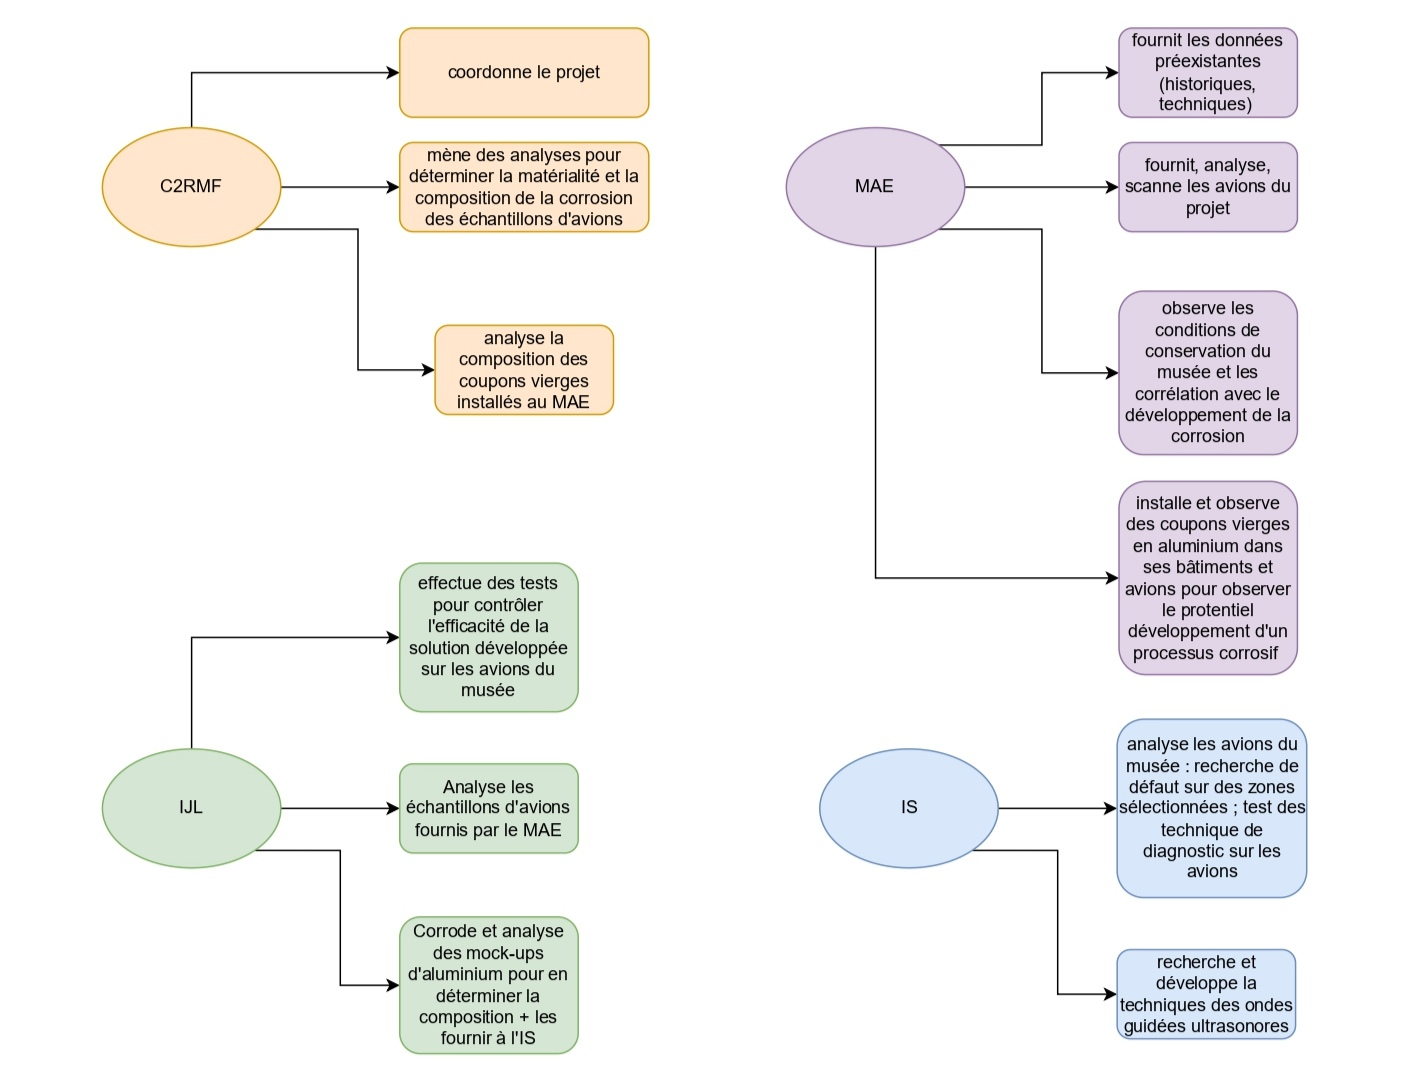
\includegraphics[width=1.4\textwidth, angle=90]{images/roles_des_acteurs.jpg}
    }
    \caption{Le rôle des acteurs du projet C-ADER}
\end{figure}


    \secwithshorttitle{Les objets étudiés}{Les objets étudiés : avions, échantillons, mock-up}{Les objets étudiés : avions, échantillons, mock-up}
    
Les recherches de ce projet seront menées sur plusieurs types d'objets qu’il convient de présenter. Les premiers -et les plus importants- éléments à être analysés sont six avions du Musée de l’Air et de l’Espace. Ces avions sont constitués majoritairement d’alliages 2XXX à base d’aluminium-cuivre contenant des traces de fer et de manganèse, abrégé Al-Cu (Fe-Mn). Ce choix est justifié par la volonté d'étudier des avions aussi bien entreposés en intérieur qu’à l’extérieur, et dont l'état de dégradation est varié. On trouve : 

\begin{itemize}
    \item Deux Boeing 707, le « château de Maintenon » (dont il ne reste plus que l’avant du fuselage) conservés dans un hangar, et le « château de Dampierre », conservé quant à lui dans son intégralité en extérieur, issus tous deux de la flotte des Boeing « Châteaux in the Sky » de la compagnie Air France.
    \item Un Morane Paris, plus précisément un Morane-Saulnier MS. 760 Paris,
    \item Un autre Boeing, mais cette fois-ci un B17G, conservé dans un hangar,
    \item Deux Mirages IV, un conservé en extérieur et très largement corrodé, et un autre conservé en intérieur.
\end{itemize}

L’appareil sélectionné pour la réalisation d’un premier jumeau numérique est le Boeing 707 « Château de Maintenon ». Il convient de préciser que seul le nez de l’appareil ayant été conservé par le musée, sa représentation numérique est susceptible de ne faire figurer que la partie existante actuellement, et non l’intégralité de l’avion. Par sa nature même, cette section est plus accessible pour la réalisation d’analyses, permettant ainsi des prélèvements directs sur le fuselage.\\

Un avion entier n’a pas vocation à être analysé sur place, c'est-à-dire au Musée de l’Air et de l’Espace, par tous les acteurs impliqués dans le projet. Seuls le service restauration et conservation du musée, ainsi que l’Institut de Soudure au début du projet, seront amenés à y travailler, l’objectif pour l’Institut de Soudure étant d’identifier des potentiels défauts présents sur les zones de travail sélectionnées sur chaque avion.\\

Les différents acteurs du projet travailleront dans un premier temps sur des prélèvements -appelés échantillons- provenant de plusieurs avions. Le Centre de recherche et de restauration des musées de France (C2RMF) et l’Institut Jean Lamour (IJL) mèneront de concert des examens afin de caractériser la composition, la morphologie et le niveau de dégradation des échantillons prélevés. À partir des données collectées sur ces derniers des échantillons modèles (mock-up) seront préparés. Ces mock-up constitués d’alliages d’aluminium 2024 seront artificiellement corrodés afin de reproduire les faciès de corrosion observés. C’est sur ces échantillons modèles que seront dans un premier temps testées à la fois les techniques d’analyse non destructive à base d’ondes guidées et les méthodes de protection contre la corrosion. Ces techniques et traitements seront finalement mis en œuvre sur les aéronefs sélectionnés pour validation finale.\\

La connaissance de ces types d’objets et des échanges qui vont s’effectuer entre les différents partenaires sera ainsi essentielle pour l’étude des données produites et la conception des outils de valorisation du projet C-ADER.

\clearpage % Force le saut de page

\begin{figure}[H]
    \centering
    \makebox[\textwidth][c]{%
        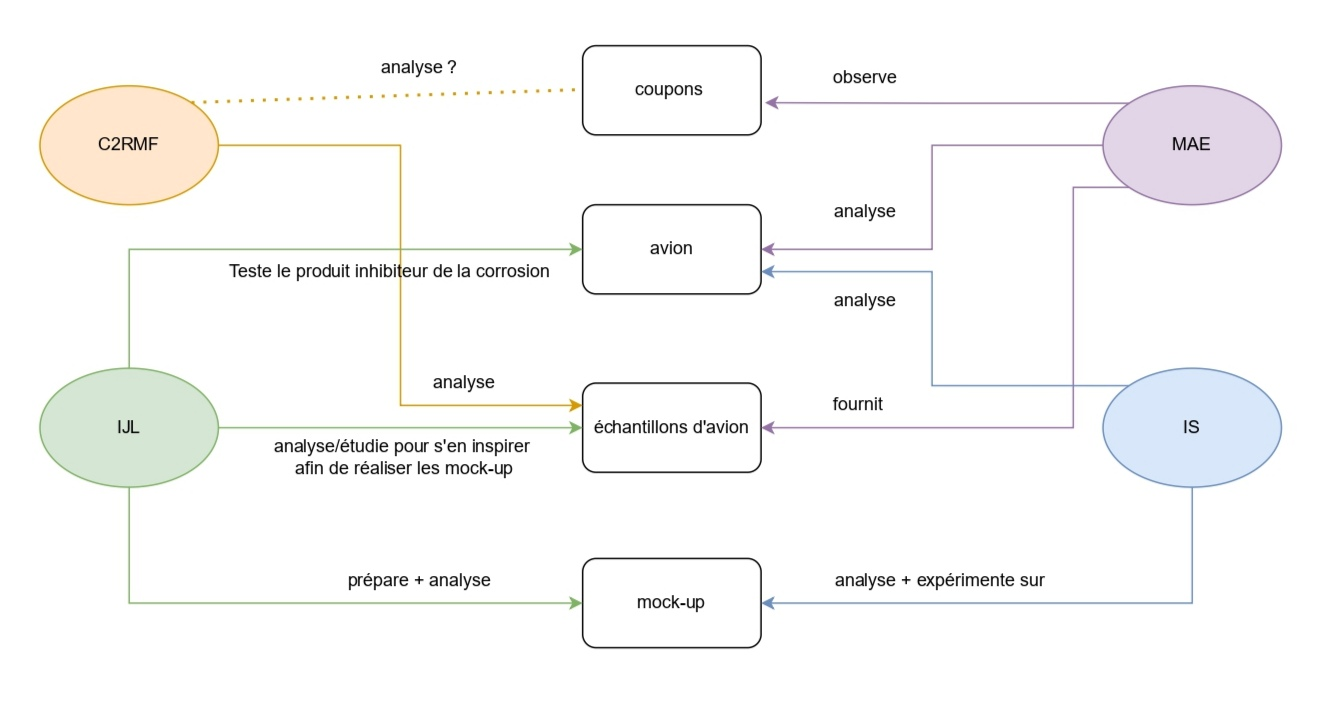
\includegraphics[width=1.4\textwidth, angle=90]{images/objets_etudies.jpg}
    }
    \caption{Les objets étudiés}
    \label{fig:votre_label2_ici}
\end{figure}

    
     \clearemptydoublepage
     
    \chapwithshorttitle{Concepts, technologies, applications}{Le jumeau numérique : concepts, technologies et application}{Le jumeau numérique : concepts, technologies et application}  
Avant de se pencher sur le traitement des données dans le cadre d'un projet de recherche, il est pertinent d'examiner le concept de jumeau numérique vers lequel ce projet tend. Cette réflexion préliminaire permet de mieux définir ce concept et d'ajuster la gestion des données en conséquence.

    \secwithshorttitle{Historique et définitions}{Historique et définition du jumeau numérique}{Historique et définition du jumeau numérique}

        \subsection{Émergence et évolution d’une technologie prometteuse}

L’idée maîtresse du concept de jumeau numérique remonte aux années 1960. La NASA développe ce qui est aujourd'hui considéré comme l'ancêtre des jumeaux numériques pour ses missions d'exploration spatiale. Lors de la mission Apollo 13, une réplique exacte du vaisseau était présente sur Terre, permettant aux scientifiques de réaliser des tests et de proposer aux astronautes les meilleures solutions lorsque les réservoirs d'oxygène explosèrent en plein vol.\footcite{QuEstceQu2023}\footcite{miskinisMysteriousHistoryDigital2019}

Le concept reste en suspens mais n'est pas réellement exploité. C'est en 1991, lorsque David Gelernter publie Mirror Worlds\footcite{gelernterMirrorWorldsDay1991}, que sont posées les bases conceptuelles de ce qui deviendra plus tard la technologie du jumeau numérique.\footcite{kalilMirrorWorldsBook2024} Gelernter imagine des « mirror worlds », où des systèmes réels comme des villes, des écosystèmes ou des processus industriels sont fidèlement reproduits dans un environnement numérique. Ces mondes numériques reflètent en temps réel l'état de leur homologue physique, offrant ainsi une observation directe des phénomènes à l’échelle micro ou macroscopique. Plus encore, dans ces « mirror worlds », les utilisateurs peuvent interagir avec les systèmes représentés, permettant de comprendre les interactions entre les différents composants. Ces mondes miroirs offriraient une surveillance continue et une gestion proactive des systèmes, permettant d’anticiper les problèmes, d’optimiser les performances, et de prendre des décisions éclairées basées sur des données en temps réel. Gelernter envisageait déjà des applications dans divers domaines, tels que la gestion urbaine, la médecine, l'éducation et les entreprises.\footcite{zadehDigitalTwinMight2024}  Il est néanmoins trop visionnaire pour son époque, alors qu'Internet en est encore à ses débuts. Bien que sa technologie soit saluée par le New York Times, elle reste largement ignorée.\footcite{lehmann-hauptBooksTimesMirror1991}\\

Son idée semble être délaissée. Ce n'est que sept ans plus tard que la dénomination « digital twin » apparaît pour la première fois en 1998, alors qu'elle est utilisée pour désigner une copie numérique de la voix de l'acteur Alan Alda dans le projet intitulé Alan Alda meets Alan Alda 2.0. Ce projet visait à montrer l’acteur en train d’interagir avec une version virtuelle de lui-même,  afin de mettre en avant la façon dont les doublons numériques pouvaient être utilisés dans les médias et le monde du divertissement.\footcite{miskinisMysteriousHistoryDigital2019}\footcite{onceaDigitalTwinsApollo2024} Sans pour autant atteindre l'idée d'un monde virtuel numérique double, le principe de jumeau continue de séduire.\\

C'est en 2002 qu'un nouveau pas est franchi. Michael Grieves, professeur à l'université du Michigan, réalise une présentation. Son but est de rendre les usines et leur fonctionnement plus efficaces, et selon lui, la clé réside dans la création d’une réplique virtuelle parfaitement fidèle de chaque élément physique. Machines, chariots élévateurs, et même travailleurs, tout pourrait être analysé sur un écran d'ordinateur. Ce modèle virtuel serait alimenté en continu par un flux de données, se mettant à jour en temps réel pour refléter avec précision l’usine. Il décrit alors toutes les caractéristiques d’un jumeau numérique moderne : un espace réel, un espace virtuel, la diffusion des données et l’interaction entre les deux types d’éléments.\\

Il faut de nouveau attendre quasiment une décennie pour que la définition du jumeau numérique gagne en précision. En 2010, John Vickers introduit le terme « jumeau numérique » dans un rapport de feuille de route de la NASA intitulé  Technology Area 12 : Materials, Structures, Mechanical Systems, and Manufacturing Road Map (domaine technologique 12 : matériaux, structures, systèmes mécaniques et fabrication). Cette fois-ci, le terme est associé à l'idée qu'on lui donne habituellement. La technologie est définie comme une représentation virtuelle d'un objet ou d'un processus, qui permet de simuler et d'analyser le comportement et les performances de l'objet ou du processus réel. Selon ce rapport, le concept de jumeau numérique se compose de trois parties distinctes : l'objet ou le processus physique et son environnement physique, la représentation numérique de l'objet ou du processus, et le canal de communication entre les représentations physique et virtuelle. Les connexions entre la version physique et la version numérique incluent des flux d'informations et de données, y compris des flux de capteurs physiques entre les objets et environnements physiques et virtuels\footcite{JumeauxNumeriquesGuide}. \\

Avec l'utilisation de plus en plus aisée d'Internet, qui permet l'échange des données en temps réel, et l'évolution de la technologie IoT (Internet of Things), qui désigne les dispositifs connectés qui relient les éléments physiques à leur représentation numérique\footcite{thermosJumeauNumeriqueConcept2024}, l'utilisation des jumeaux numériques devient de plus en plus attractive. C’est ainsi que le concept fleurit très largement dans le courant des années 2020. Un article de 2022 intitulé « Digital Twins: Potentials, Ethical Issues, and Limitations » va même jusqu'à constater que « créer des jumeaux numériques à propos de tout devient une idée attractive »\footcite{helbingDigitalTwinsPotentials2022}. Enfin, le World Economic Forum labellise en 2024 le jumeau numérique comme faisant partie de la « quatrième révolution industrielle », l’inscrivant définitivement au panthéon des nouvelles technologies révolutionnaires.\footcite{batagliaWhyTeamingIndustry2024}.\\

Il est intéressant de noter qu'au cours du développement du jumeau numérique dans l'histoire, trois grandes périodes tendent ainsi à se dégager, périodes où un jumeau numérique ne voulait pas forcément faire référence à une même technologie. Des années 60 jusqu’en 2002, un jumeau numérique est une représentation numérique d’d'un élément concret alimenté par des données pour le rendre aussi réaliste que possible. De 2003 à 2014, le concept s'affine pour inclure des simulations basées sur les résultats de mesures collectées via des capteurs afin de disposer de données à tout instant. Depuis 2015, un jumeau numérique désigne un objet physique connecté en permanence au virtuel, avec une interaction bidirectionnelle : l'objet physique influence l'objet numérique, et vice-versa.\footcite{grievesJumeauxNumeriquesPresentation2019}

 \subsection{La définition du jumeau numérique de nos jours}

    \subsubsection{Définition}

Avant de présenter ce qu'est un jumeau numérique, il convient de préciser que les sources disponibles à ce sujet sont assez rares. Il s'agit en effet d'un sujet niche, dont la définition technique assez complexe semble vouée au changement. En outre, la plupart des présentations techniques des jumeaux numériques se trouvent sur des sites d'entreprises qui offrent leurs services pour en construire, ou sur des blogs intéressés par les évolutions numériques offertes par la technologie, dont les définitions peuvent varier. Les informations qui y sont exposées visent donc à présenter ce qu'est un jumeau numérique dans les grandes lignes, les capacités qu'il offre, mais parlent rarement d'une définition consensuelle. Le jumeau numérique est avant tout considéré comme un outil exploité par le secteur industriel, et commence seulement à gagner en intérêt pour le domaine patrimonial. Par conséquent, si cette technologie a pu faire l'objet de recherches scientifiques, elle est très largement abordée sous un point de vue scientifique et technique, et quasiment jamais patrimonial. Seuls quelques articles commencent à fleurir à ce sujet à partir des années 2010 - 2020, mais ces derniers restent rares.\\

Il est donc ardu de définir précisément ce qu’est un jumeau numérique. La plupart des articles qui tentent d’en fournir une définition se contentent d’énoncer les différentes fonctionnalités qu’il peut offrir\footcite{MiroirMiroirJumeau2021}. Néanmoins, le point principal qui revient systématiquement laisse entendre qu’un jumeau numérique cherche à reproduire tout élément, qu’il s’agisse d’un système, d’un processus, ou d’un objet qui nécessite d’être dupliqué afin d’être étudié.\footcite{miskinisComparingInternetThings2018}. La plupart des définitions proposées convergent vers les mêmes concepts fondamentaux : un modèle physique existant dans ce qui est appelé le « monde réel », un modèle numérique, une interaction entre les deux, et la transmission des données.\\

En outre, aucune définition consensuelle n’a encore émergé au sein de la communauté scientifique. Ce n’est qu’en 2023, que le Digital Twin Consortium propose une définition formelle. Créé en mai 2020, le Digital Twin Consortium (ou DTC) est une organisation mondiale dédiée à la promotion et au développement de cette technologie\footcite{DigitalTwinConsortium}. En collaboration avec l'industrie, le gouvernement et le milieu académique, il cherche à devenir l'autorité en matière de jumeaux numériques en le définissant, en comblant les lacunes technologiques et en publiant des normes, des architectures et des avis. L'objectif est de standardiser la technologie des jumeaux numériques pour qu'elle puisse être utilisée efficacement dans divers secteurs.  Sa définition est la suivante :\\

\begin{quote}« A digital twin is a virtual representation of real-world entities and processes, synchronized at a specified frequency and fidelity.
\begin{itemize}
\item Digital twin systems transform business by accelerating holistic understanding, optimal decision-making, and effective action.
\item Digital twins use real-time and historical data to represent the past and present and simulate predicted futures.
\item Digital twins are motivated by outcomes, tailored to use cases, powered by integration, built on data, guided by domain knowledge, and implemented in IT/OT systems. »\footcite{DefinitionDigitalTwin}
\end{itemize}
\end{quote}

D'après cette définition, un jumeau numérique est une « représentation virtuelle d’entités et de processus du monde réel, synchronisée à une fréquence et une précision données ». Cette définition large, est secondée ici par les fonctionnalités offertes par un jumeau numérique, à savoir la possibilité d’accélérer la compréhension globale d’un système et d’optimiser la prise de décision.\\ 

Le deuxième point soulève une particularité intéressante : pour exister, un jumeau numérique se base sur plusieurs types de données, à savoir des données déjà produites et des données en temps réel. C'est ce qui rend la technologie fascinante : un jumeau numérique est capable de représenter à la fois le passé d’un objet, mais aussi son état actuel et son état à venir. Par exemple, le jumeau numérique d’un avion représenterait non seulement les vols effectués par le passé, l’état de ses moteurs et de son fuselage, mais aussi l’état de ses pièces dans un certain nombre d’années en fonction des données récoltées. Cela implique que l'élément réel soit équipé de capteurs qui permettent au jumeau numérique de récolter ses données et de suivre en temps réel son état tout en évoluant avec lui\footcite{gladieuxJumeauNumeriqueAeronautique2019}.\\ 

Enfin, le dernier volet de cette définition vient rappeler qu’un jumeau numérique n’est pas orienté vers la simple représentation d’un objet ou d’un processus (ce qu'une modélisation pourrait faire), mais davantage vers les résultats produits grâce aux données récoltées et aux analyses effectuées. Il agrège les connaissances disponibles, les données et les simulations relatives au système en question grâce à des capteurs notamment, offrant une analyse approfondie et une anticipation des comportements futurs en s'adaptant aux données en temps réel provenant de l'actif physique\footcite{bealJumeauNumeriqueRealite}\footcite{QuEstceQu2023}.\\

Cette définition met ainsi en avant le type de données qui constituent un jumeau numérique, et qu'il sera intéressant de repérer lors de la gestion des données du projet C-ADER : 
\begin{itemize}
    \item \textbf{Les données actuelles}, c’est-à-dire des données en temps réel provenant des capteurs de l’équipement, des sorties des plateformes et systèmes de fabrication, ainsi que des systèmes de la chaîne de distribution. On pense par exemple aux données de la plateforme « Virtual singapor », qui est sans cesse alimentée par des informations collectées visant à mesurer la qualité de l’air et la température. Dans le cadre du projet C-ACER, il s’agira davantage des données d’analyses effectuées sur les avions du projet, même s’il s’agit plutôt dans la globalité de relevés concernant un instant T, et non pas de relevés en continu. 
    \item \textbf{Les données historiques}, qui comprennent les performances passées des machines, des processus et des systèmes, ou les données retraçant la vie de l’objet réel modélisé. C’est par exemple les données de maintenance des flottes de l’armée de l’air et de la marine nationale, collectées par Dassault aviation et mises dans 3DExperience pour venir alimenter les JN de chaque appareil. Pour C-ADER, on trouverait l’équivalent dans la documentations et les archives relatives à des incidents techniques ou à des réparations d’avions susceptibles de renseigner sur l’état des appareils ; il pourrait également être question de documents relatant les historiques de vols, ou bien plus concrètement les plans et les documents relatifs au système technique de l’appareil.
    \item \textbf{Les Données prédictives} produites par le jumeau numérique lui-même. Issues de l'apprentissage automatique, elles projettent les performances et les comportements attendus. Ce type de données sera absent des jumeaux numériques prévus dans le cadre du programme C-ADER\footcite{rebecchiQuEstceQue2021}.\\ 
\end{itemize}

À la fois outil centralisateur de données, planificateur, ces spécificités font du jumeau numérique un outil qui permet d'accéder à toutes les informations sur l'objet ou le processus représenté sans avoir besoin de l'avoir physiquement à disposition. 

        \subsubsection{Les principes garants de l'efficacité d'un jumeau numérique}

Un jumeau numérique doit respecter plusieurs principes au commencement de sa conception, qui sont essentiels pour garantir l’efficacité de l’outil et qu'il est nécessaire de connaître avant de se pencher sur les types de données à traiter.\\

\begin{enumerate}
    \item Conception Simultanée : Ce principe consiste à développer le modèle numérique et le système physique en même temps. Cette approche assure une synchronisation continue entre le jumeau numérique et son équivalent physique, permettant des ajustements en temps réel et une meilleure intégration des modifications. Par exemple, si on construit un nouvel avion, on crée en parallèle une version numérique qui évolue avec l’avion réel. Cela permet de s'assurer que toutes les modifications apportées à l'avion réel sont également mises à jour dans la version numérique, et vice-versa. Cela permet de détecter et de corriger rapidement des problèmes potentiels.\\
    \item Représentativité : Le jumeau numérique doit représenter fidèlement le système dans son ensemble et reproduire son comportement dans diverses conditions. La représentativité comprend deux sous-critères :
    \begin{itemize}
        \item Expressivité : Capacité à décrire divers phénomènes et scénarios possibles. Cela signifie que le modèle doit être suffisamment détaillé et flexible pour simuler une large gamme de situations, allant des conditions normales aux événements exceptionnels. Par exemple, il doit pouvoir montrer comment l’avion se comporte en vol, lors de l’atterrissage ou dans des conditions météorologiques extrêmes.\\
        \item Précision : Écart minimal entre les résultats simulés et les mesures réelles. Une haute précision assure que les simulations fournies par le jumeau numérique sont fiables et peuvent être utilisées pour des prévisions et des décisions critiques. Par exemple, si l’avion réel consomme 5 litres de carburant par minute en vol, le jumeau numérique doit montrer la même consommation.\\
    \end{itemize}
    \item Interopérabilité : Le jumeau numérique doit pouvoir se connecter et fonctionner avec d'autres applications, jumeaux numériques, ou capteurs physiques. Cette capacité garantit une intégration fluide avec les systèmes existants et futurs, permettant une communication et un échange de données efficaces entre différents composants et plateformes.\\
    \item Présence : Ce critère évalue la capacité du jumeau numérique à permettre à un humain de percevoir et d'interagir avec le système. La réalité virtuelle joue un rôle crucial en offrant une immersion sensorielle dans un environnement simulé. Les utilisateurs peuvent interagir avec le jumeau numérique via divers contrôles tels que la voix, les manettes ou la capture de mouvements, améliorant ainsi l'expérience utilisateur et l'efficacité des formations et des simulations.\\
    \item Explicabilité : Le jumeau numérique doit être transparent et facile à comprendre. Cela signifie qu'il doit être possible d'expliquer comment il fonctionne et pourquoi il donne certains résultats. Cela implique une transparence totale dans les opérations et les processus, facilitant la recherche de solutions en cas de dysfonctionnements et l'optimisation des performances. Par exemple, si le jumeau numérique montre une défaillance dans une pièce de l’avion, il doit être possible de retracer les données et les simulations pour comprendre pourquoi cette défaillance est prévue et comment elle peut être corrigée.\\
    \item Autonomie : Le jumeau numérique doit reproduire fidèlement le comportement du système physique et s'adapter à un large éventail de conditions pour permettre au jumeau numérique d'anticiper et de réagir à des situations exceptionnelles avant qu'elles ne se produisent sur le système physique. Cela inclut la capacité à prendre des décisions basées sur des analyses prédictives et à effectuer des ajustements autonomes pour prévenir des pannes ou optimiser les performances. Par exemple, il doit pouvoir surveiller en continu l’état de l’avion et déclencher des alertes ou des actions correctives sans intervention humaine si un problème est détecté. Cela permet de réagir rapidement aux situations imprévues et de minimiser les risques.\footcite{bealJumeauNumeriqueRealite}
\end{enumerate}

Ces éléments devront ainsi être traités avec considération lors du traitement et de la structuration des données du projet C-ADER lors de leur modélisation.

    \secwithshorttitle{Caractéristiques et potentiels}{Caractéristiques et potentiel des jumeaux numériques}{Caractéristiques et potentiel des jumeaux numériques}
        \subsection{Des fonctionnalités multiples}

Dans toutes les définitions de jumeau numérique qu’on peut trouver, ce sont avant tout les fonctionnalités de l’outil qui sont mises en avant. Sans pour autant se vouloir exhaustives, ces principales possibilités permettent aussi d’expliciter davantage ce qu’est un jumeau numérique.

            \subsubsection{Centraliser, clarifier et mettre en valeur les informations}

Le jumeau numérique est un outil puissant pour la mise en commun des données. Il centralise des informations choisies et préalablement collectées en fournissant une plateforme collaborative où les différentes parties prenantes peuvent se connecter et échanger. Il agit comme un agrégateur de données : il fédère les données et les structure dans un environnement commun. Il facilite la synthèse des connaissances et améliore la coordination entre les acteurs impliqués. Par sa capacité à faire interagir les données de différents domaines, le jumeau numérique va aider à fluidifier les échanges entre des experts de différents secteurs d'activité. Un jumeau numérique est par conséquent une aide précieuse pour l’échange et le partage des informations.

            \subsubsection{Aide à la conception}

Les jumeaux numériques jouent un rôle clé dans la conception d'objets, d'éléments ou de processus. En fournissant une plateforme virtuelle, ils permettent de tester et d’évaluer des concepts sans avoir besoin de prototypes physiques. Ils facilitent l'évaluation des modifications avant leur mise en œuvre. Par exemple, dans l'industrie automobile, un constructeur peut utiliser un jumeau numérique pour simuler et optimiser les performances d'un nouveau modèle de voiture avant sa fabrication, ce qui aide à identifier et corriger les potentiels problèmes.

            \subsubsection{Surveiller l’élément dupliqué}

\begin{quote}«Le jumeau numérique est aujourd'hui employé pour représenter un système entier : un avion dans son intégralité, une chaîne logistique, une usine, etc.»\footcite{garcia-monteroJumeauNumeriqueQu2023}.
\end{quote}

Il constitue un outil de gestion de son homologue physique en suivant les phases de son cycle de vie en temps réel. Ils sont ainsi conçus pour pouvoir assurer le pilotage et la surveillance à distance des éléments qu'ils représentent, et se sont distingués dans la maintenance.

            \subsubsection{Analyser et prévoir}

Ces capacités leur permettent d'effectuer des retours d'expérience : ils donnent la possibilité de rejouer et d'analyser le comportement du système à partir des données archivées. Le jumeau numérique permet également de créer des simulations et d’explorer des scénarios alternatifs, en se basant d’une part sur l'historique, l'état actuel et les prévisions futures du système. Cela aide à anticiper les évolutions et les défis futurs en testant différentes possibilités avant qu'elles ne se produisent réellement\footcite{donniniToutComprendreJumeau2023}. Ces scénarios permettent donc d’adopter une approche proactive, plutôt que réactive, et d'anticiper.\\

Un jumeau numérique serait vraisemblablement un outil polyvalent et capable d'apporter une réelle plus value à l'élément qu'il modélise. Aussi polyvalent et multiples que ses usages, il existe plusieurs types de jumeaux numériques.

        \subsection{Une multiplicité d'approches et de points de vue}

Deux méthodes de traitement et d'utilisation des données différentes se dégagent : l'approche top-down et l'approche bottom-up.

            \subsubsection{Approche top-down (descendante) }

Cette approche commence par des modèles théoriques basés sur des principes physiques, qui sont ensuite raffinés en intégrant des données réelles pour prédire le comportement d'un système spécifique. Elle est conçue avec des équations et des modèles fondés sur des principes physiques. Ces modèles sont souvent issus de la mécanique, de la thermodynamique, de l'électromagnétisme, etc. Les équations physiques sont résolues numériquement à l'aide de logiciels de simulation pour prédire le comportement de l'actif ou du système sous différentes conditions. Par la suite, les mesures réelles peuvent être intégrées pour ajuster et affiner ces simulations. Les résultats de la simulation peuvent être comparés aux données réelles pour valider le modèle et améliorer sa précision. Cette approche pourrait être comparée à un raisonnement inductif, en partant de modèle généraux pour s’adapter au cas particulier de l’élément modélisé. Un problème potentiel de cette approche est qu'elle peut faire disparaître certains éléments, puisqu’elle simplifie les données observables et part d’un modèle général.\\

Le jumeau numérique d’un pont pourrait par exemple être conçu suivant cette approche. Ce pont serait construit en fonction de propriétés mathématiques et architecturales. À l'aide de logiciels de simulation, ces propriétés sont testées et mises en contexte pour prédire comment le pont se comportera sous différentes charges, en fonction des conditions météorologiques. L’idée est donc bien de partir de principes généraux pour ensuite l’appliquer à une situation particulière.\\

Par conséquent, dans cette approche, les données sont principalement utilisées pour valider et affiner des modèles théoriques préexistants. Les traitements se concentrent sur l'ajustement des simulations numériques pour qu'elles correspondent aux observations réelles, et l'accent est mis sur la résolution d'équations complexes ou d'intégration de données, de manière à affiner les prédictions du modèle.

            \subsubsection{Approche bottom-up (ascendante)}

Cette méthode part des données collectées directement sur un actif physique, en utilisant des capteurs et des techniques d'IA pour construire un modèle numérique capable de prédire et d'optimiser son fonctionnement en temps réel. La conception du jumeau numérique part de l'élément concret à modéliser. Cet élément, généralement un objet ou une machine, est équipé lorsque cela est possible de capteurs qui collectent des données en temps réel concernant son état et son fonctionnement. Les données collectées sont ensuite utilisées pour effectuer la modélisation et concevoir l’architecture des modèles numériques. Cette approche fait souvent intervenir des techniques d'intelligence artificielle (IA) comme le machine learning (apprentissage automatique), le deep learning (apprentissage profond) ou les réseaux de neurones, pour prédire comment l’actif se comportera dans diverses situations. Contrairement à l’approche top-down, l’approche bottom-up peut être comparée à un raisonnement déductif, qui partirait d’un objet ou processus particulier, et qui s'élargirait au fur et à mesure.\\

Cette approche pourrait être intéressante dans le cadre de la réalisation d’un jumeau numérique destiné à surveiller un moteur de voiture par exemple. Il serait équipé de capteurs visant à collecter les données en temps réel pendant son fonctionnement (par exemple la température, la pression d’huile, les vibrations). À partir de ces données, un modèle numérique du moteur serait construit. Ce modèle pourrait prédire quand certaines pièces du moteur seraient sur le point d’être trop usées voire défectueuses, permettant ainsi d’anticiper les pannes et d'effectuer la maintenance nécessaire avant que des problèmes majeurs surviennent.\\

Ces deux approches peuvent également être utilisées de façon complémentaires. On parle dans ce cas d’approche mixte.\footcite{bealJumeauNumeriqueRealite}\footcite{garcia-monteroJumeauNumeriqueQu2023}\\

Dans le cadre du projet C-ADER, l’approche à déterminer est encore à discuter. On pourrait ainsi estimer que l’approche top-down sera la plus efficace, puisque le travail de modélisation en cours cherche à représenter une architecture idéale et applicable à tous les types d’avions analysés au cours du projet, et ne part pas d’un avion précis et de ses données respectives avant de construire un modèle numérique.

 \subsection{Typologie des jumeaux numériques }

 Il existe plusieurs types de jumeaux numériques, en fonction de l’élément modélisé qu’ils représentent. Bien qu'ils ne soient pas recensés par le Digital Twin Consortium, probablement afin de ne pas se limiter à des dénominations techniques vouées à évoluer, on trouve quatre types principaux qui ressortent des diverses définitions et articles sur la question :\\

\begin{figure}[ht]
    \centering
    \adjustbox{max width=\textwidth}{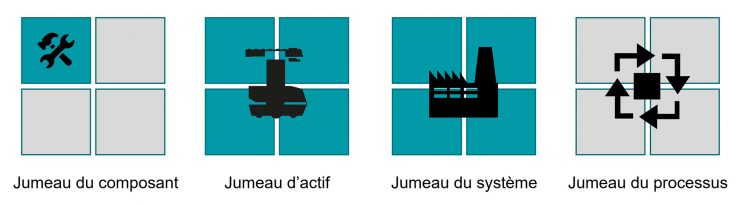
\includegraphics{images/types-de-jumeaux-numeriques.jpg}}
    \caption{Les différents types de jumeau numérique}
    {source : Jumeau numérique en logistique, KNAPP\footcite{JumeauNumeriqueLogistique2023}}
\end{figure}

\begin{itemize} 
 \item \textbf{Jumeaux de composant (component twins, ou part twins)} : Les jumeaux de composant sont la représentation numérique d'une seule pièce qui assure une fonction clé dans d'un système complet. Il peut s’agir par exemple d'un moteur dans une éolienne. 
 \item \textbf{Jumeaux d'actif (asset twins)} : Un actif est un élément individuel, souvent une machine ou un équipement, qui peut faire partie d'un système plus vaste. Un jumeau d'actifs revient à représenter la combinaison de deux composants (les actifs) ou plus qui fonctionnent ensembles. Ce type de jumeau numérique représente un seul équipement ou une machine spécifique, ou un ensemble de composants qui fonctionnent ensemble comme une unité unique. Par exemple, un jumeau d'actif pourrait représenter comment le moteur et les pales d'une éolienne travaillent ensemble pour produire de l'énergie.
 \item \textbf{Jumeau de système ou jumeau d’unité (system or unit twins)} : il s’agit de la représentation de diverses ressources dans un même système. Le jumeau numérique fournit et met en commun des informations sur l’interaction des installations et sur des améliorations possibles de la performance, par exemple de la production globale. Ce type de jumeau numérique représente un ensemble plus large et complexe de machines ou d'équipements, souvent au niveau d'une installation entière ou d'un processus global.
 \item \textbf{Jumeaux de processus (process twins)} : Les jumeaux de processus sont des représentations numériques des procédures et des flux de travail, plutôt que des représentations d’un produit physique. Ils modélisent, au sein d’un environnement numérique, comment les différents composants, équipements et unités interagissent et fonctionnent ensemble. Ils indiquent comment les système fonctionne pour créer une installation de production globale. Par exemple, un jumeau de processus peut reproduire le fonctionnement complet d'une usine de fabrication, incluant tous les composants et machines qu'elle contient. Cela permet d'analyser et d'améliorer les processus opérationnels, d'identifier les inefficacités et de tester des changements sans affecter l'environnement réel. \footcite{QuEstceQu2023}\footcite{JumeauNumeriqueLogistique2023}
\end{itemize}

Pour résumer, un jumeau numérique peut donc représenter : une seule pièce d’un produit, plusieurs pièces ou composants qui fonctionnent ensemble, un système complet, un processus.\\

Parmi ces distinctions, d’autres types de jumeaux numériques de distinguent. Ils sont quant à eux définis par le moment où ils sont créés, c'est-à-dire avant, pendant ou après la création du produit\footcite{DigitalTwin2024} \footcite{rebecchiQuEstceQue2021}.\\

\begin{itemize}
    \item \textbf{Prototype de jumeau numérique (digital Twin prototype)} : Ce type se compose des conceptions, analyses et processus nécessaires à la réalisation d'un produit physique. Utilisé avant la création du produit, il permet de tester et d'optimiser les caractéristiques du produit dans un environnement virtuel avant sa fabrication.
    \item \textbf{-	Instance de jumeau numérique (Digital Twin Instance)} : Une fois que le produit est fabriqué, ce jumeau numérique représente chaque instance individuelle du produit. Il est lié à son homologue physique pour toute la durée de vie de ce dernier, permettant de réaliser des tests sur différents scénarios d'utilisation et de surveiller la performance en temps réel.
    \item \textbf{-	Agrégat de jumeau numérique (Digital Twin Aggregate)} : Ce type regroupe les informations provenant des différentes instances de jumeaux numériques (DTI). Ces données peuvent être utilisées pour des interrogations sur le produit physique, des pronostics et des apprentissages. L'agrégat permet de déterminer les capacités globales d'un produit, d'effectuer des prévisions et d'optimiser les paramètres de fonctionnement.\\
\end{itemize}

On peut estimer que le projet C-ADER utilisera le modèle du jumeau de composant ou de pièce. En effet, les jumeaux de composant ou de pièce se concentrent sur des parties individuelles d'un système plus vaste. Justement, l’objectif pensé pour la réalisation du jumeau numérique est de rendre chaque partie de l'avion scannée (donc chaque composant unique) cliquable. Chaque partie de l'avion serait numérisée et rendue interactivement accessible, permettant aux utilisateurs d'explorer des informations détaillées sur chaque composant individuel. Cette approche correspond étroitement à la définition des jumeaux numériques de composant ou de pièce, où l'accent est mis sur la granularité des données et la possibilité d'accéder à des détails spécifiques sur les éléments constitutifs.\\

En raison de la nature statique de l'avion exposé dans un musée, les composants individuels ne subissent pas de changements dynamiques fréquents. Cette caractéristique est typique des jumeaux de composant plutôt que des jumeaux de processus ou de systèmes, qui sont davantage orientés vers la gestion et l'optimisation de processus dynamiques en temps réel.  De même, les jumeaux de systèmes ou d'unités, qui se concentrent sur l'assemblage fonctionnel de divers actifs pour améliorer les performances globales, semblent mieux adaptés à des environnements opérationnels et dynamiques. Enfin, les jumeaux de processus, qui suivent et optimisent les flux de travail dynamiques, ne s'appliquent pas directement à un avion exposé comme c'est le cas.\\

Ces différents types et approches témoignent ainsi de la grande flexibilité de l'outil, ce qui contribue à expliquer la très large popularité de cet outil dans des cadres assez variés.\\

 
    
     \clearemptydoublepage
     
    \chapwithshorttitle{Cas d'usage : industrie, patrimoine}{Cas d'usage des jumeaux numériques : de l’industrie au patrimoine}{Cas d'usage des jumeaux numériques : de l’industrie au patrimoine}  

Si le concept de jumeau numérique s'est rapidement développé ces dernières années, il est intéressant de consulter quelques exemples, aussi bien dans le cabre industriel que patrimonial, pour mieux comprendre à quoi l'outil numérique du projet C-ADER sera susceptible de ressembler à la fin du projet.

        \secwithshorttitle{Dans l'industrie}{Développement et usage dans le secteur industriel}{Développement et usage dans le secteur industriel}

C’est dans le secteur industriel qu’est très largement portée l’utilisation du jumeau numérique. Il est intéressant de se pencher sur les utilisations qui en sont faites, dans le secteur aéronautique principalement, mais également dans d'autres secteurs afin de saisir l'importance de cette technologie de nos jours, et expliquer son engouement pour le projet C-ADER.\\

Les entreprises les plus prolifiques dans ce domaine sont General Electric, avec Predix ; Dassault Systèmes, avec sa plateforme 3Dexpérience, et Siemens, avec le logiciel SIMIT, dont le nom revient de nombreuses fois dans les exemples de jumeaux proposés. Leurs noms reviendront ainsi souvent dans les exemples proposés.\\

Un des premiers secteurs à utiliser le jumeau numérique comme outil de travail est, dans la foulée de l’aérospatial, l’automobile et l’aéronautique. Le choix a été fait de ne se pencher que sur l'aéronautique, puisque c secteur croise également le coeur du projet C-ADER.\\

À l’occasion du salon du Bourget en 2015, le patron de PTC, James Heppelmann faisait la démonstration d’un jumeau numérique à partir d’une simple maquette posée sur une table, devant les journalistes. Celle-ci représentait l’avion en exploitation, équipé de capteurs d’ouverture des portes, de thermomètres, d’un gyroscope, etc. Au mur, un écran affichait son modèle numérique répercutant en temps réel les données provenant de la maquette. L’objectif était d’avoir une représentation numérique fidèle de l’appareil exploité par le client\footcite{gladieuxJumeauNumeriqueAeronautique2019}. La même année, Airbus développait sa première maquette numérique complète d'un avion, l'A350, qui était mis en service. L'A321 connaît lui-aussi la création d'un jumeau numérique pour le pré-assemblage de son fuselage. L'entreprise continue d'utiliser cette technologie pour assurer une continuité digitale entre le design et l'utilisation des produits, en se basant sur la plateforme 3DExperience de Dassault Systèmes – plébiscitée par Airbus comme par tous les grands acteurs du secteur, tels que Boeing, Safran, Lockheed Martin–. Les bénéfices sont multiples pour les avionneurs.\\ 

Toujours d'actualité, le concept de jumeau numérique est le cœur du contrat de maintenance Ravel, pour Rafale verticalisé, signé en mai 2019 entre Dassault Aviation et la Direction de la maintenance aéronautique du ministère des Armées, pour une durée de dix ans. Dassault Aviation doit mettre en œuvre le jumeau numérique pour l’ensemble des équipements – hors moteurs et sièges éjectables qui font l’objet de contrats distincts – des 152 Rafale de l’armée de l’air et de la Marine nationale afin d’améliorer leur maintien en condition opérationnelle (MCO). Les données de maintenance des flottes sont récupérées puis introduites dans le jumeau numérique de chaque appareil via la plate-forme 3DExperience de Dassault Systèmes, avant d'être analysées.\footcite{olivierAvionneursEmparentJumeau2020}\footcite{MirorringRealityDigital2024}\footcite{MiroirMiroirJumeau2021}.\\

Le but de ces jumeaux numérique est avant tout d'en faciliter la construction. Ils visent à anticiper et optimiser le choix des matériaux ou des pièces réalisées, grâce à la réalisation de simulations pour mieux les tester. Ils permettent également d'assurer la maintenance des appareils représentés\footcite{attaranDigitalTwinsIndustrial2024}. Le grand succès des jumeaux numérique dans l'aviation justifie ainsi le souhait du projet C-ADER de voir, à terme, un outil similaire se réaliser.\\

Le jumeau numérique fleurit également dans d'autres domaines. La logistique s'y intéresse, dans la mesure où il permet de représenter une usine entière et de la piloter, comme c'est le cas pour l'usine de l’entreprise Solvay située à Champalé\footcite{parisotCreerJumeauNumerique2015}\footcite{lawtonPremiersJoursJumeaux2021}. Le secteur du bâtiment, qui utilise déjà un outil numérique similaire, le BIM, acronyme de building information modeling, y trouve également un grand intérêt dans la gestion des villes ; on pense notamment à l'exemple type de Virtual Singapore généré en 2015 \footcite{walkerSingaporeDigitalTwin2023}, ou encore à l'échelle française, à la ville de Rennes\footcite{RennesMetropole2017} en 2017, qui ont développé chacune leur propre jumeau numérique. Enfin, le secteur de la santé s'intéresse lui aussi depuis peu aux possibilités offertes par le jumeau numérique. Une vingtaine d’approches médicales sont développées depuis 2012 sur la plateforme 3DExperience\footcite{jaliniereJumeauxNumeriquesNouveaux2021}et de nouveaux projets fleurissent, tels que le projet EDITH en 2022\footcite{SanteEcosystemeEuropeen2024}, dans le but d'étudier les possibilités de l'outil.\\

Ces différents cas viennent donc mettre en lumière la diversité des approches, des objectifs et des outils utilisés. Cette diversité est tout autant d'actualité lorsqu'il s'agit du secteur patrimonial.

        \secwithshorttitle{Dans le patrimoine}{Jumeaux numériques dans le domaine patrimonial}{Jumeaux numériques dans le domaine patrimonial}

Principalement utilisés dans la représentation de bâtiments emblématiques ou d’œuvres d’art mythiques, les jumeaux numériques développés par des institutions patrimoniales ont pour objectifs non plus la fabrication, la gestion ou la maintenance d’un produit, mais davantage la mise en valeur et la conservation de l’objet représenté, ainsi que l’accès aux données correspondantes. Contrairement à d'autres applications axées sur l'anticipation des futurs états des systèmes, l'utilisation des jumeaux numériques dans un contexte patrimonial se concentre sur la reconstitution ou la préservation du passé. 

          \subsection{Etat des lieux et perspectives }

L’usage des jumeaux numériques dans le domaine patrimonial est plus récent ; on trouve très peu de cas de jumeaux numériques recensés. En revanche, l’usage de technologies associées, à savoir la modélisation ou  la représentation 3D ainsi que le principe de réalité virtuelle tend à se démocratiser\footcite{debideranVisitesNumeriquesParcours2014} et à ouvrir la voie à l'utilisation future de jumeaux numériques. En effet, la plupart des institutions patrimoniales et culturelles ont pris conscience dès le début des années 2010 du potentiel offert par ces technologies.\\

Un pionnier dans l'utilisation de ces technologies est le site Google Art \& Culture\footcite{ExplorerGoogleArts}. Le géant d'internet a conclu plusieurs partenariats avec de grandes institutions qui lui donnent accès à leurs collections qu'il met en valeur. Quelques œuvres font l'objet d'un traitement particulier -qui peut se rapprocher de la conception du jumeau numérique- : celui d'une numérisation dont le résultat aboutit à la représentation en 3D de l'objet, et enrichi par des informations. C'est le cas notamment du David de Michel Ange\footcite{MichelangeloDavid3D}, qui avait déjà fait l'objet d'un traitement similaire dans le cadre d'une exposition en 2020 à Dubaï visant à reproduire une copie grandeur réelle en résine de la statue après plusieurs scans\footcite{lydonMichelangeloDavidHas2021}\footcite{farooqiMichelangeloDavidHas2021}. S'il ne s'agit pas encore d'un jumeau numérique, l'intérêt pour cette technologie va être rapidement exprimé.\\ 
 
C'est le cas notamment du British Museum. Grâce à son partenariat avec Google Art \& Culture, le musée avait déjà rendu accessibles et librement consultables un certain nombre de ses collections\footcite{BritishMuseumLondon}. Ses œuvres sont mises en valeur en étant accompagnées d'explications visant à les remettre en contexte, suivant le principe de visite virtuelle assez répandu dans les institutions muséales telles que le musée londonien « Victoria and Albert Museum »\footcite{ExploreCollections}. Le British Museum a cependant exploité toutes les possibilités offertes par Google Art \& Culture, en reprenant le principe de « street view »\footcite{BritishMuseumLondon}. Il est ainsi possible de se promener dans ses 85 galeries donnant accès aux collections permanentes. Le British Museum souhaite cependant pousser ses expérimentations numériques plus loin et a exprimé son intérêt pour les avantages que pouvaient offrir un jumeau numérique pour ses collections. Le projet est en cours, et un premier pas a été fait côté modélisation : le musée a scanné et mis à disposition plus de 200 objets d'arts scannés en 3D\footcite{BritishMuseum}, et consultables gratuitement, telle la célèbre pierre de rosette\footcite{RosettaStoneDownload2017}.\\ 

Ces possibilités, et tout particulièrement la modélisation 3D et l'agrégation de données, permettent donc de retranscrire la matérialité d’une œuvre à un degré dépassant celui d’une photographie en 2D. Une représentation 3D fait figurer les volumes, mais aussi -lorsque la qualité de la numérisation le permet-, les textures d’un objet, créant l’illusion de manipuler l’œuvre et de l’observer de très près, là où la muséographie ne le permet pas forcément pour des contraintes de conservation évidentes.\\

Outre les objets de collection, ce sont les sites et bâtiments patrimoniaux qui font eux aussi l'objet d'attentions particulières. En effet, de nombreux projets visent à mettre en valeur et rendre accessibles un patrimoine inconnu ou difficile d'accès.\\

CyArk\footcite{CyArk} cherche ainsi à rendre le patrimoine mondial accessible par le biais des technologies numériques 3D. Plusieurs sites sont ainsi reproduits numériquement en se basant sur le principe de photogrammétrie terrestre et aérienne, enrichis de documentations permettant de les consulter et d'en apprendre davantage, le but étant de favoriser une expérience immersive, mais aussi de permettre aux professionnels du patrimoine et de la conservation de s’en servir. Le projet invite enfin au libre échange des données, suivant le principe de l'open data. Bien que représentant une prouesse technologique et offrant d'excellentes résolutions de sites archéologiques ou patrimoniaux, comme en témoigne l’exemple de Pétra\footcite{AdDeirMonastery}, le site est davantage conçu pour le grand public que pour les professionnels de la conservation. En effet, la documentation des éléments privilégie une perspective adaptée aux besoins des amateurs plutôt qu'à ceux des scientifiques et des conservateurs.\\

C'est encore le cas avec les recherches menées par le projet ScanPyramids, qui vise à étudier la structure de quatre pyramides (les pyramides Sud, pyramides Nord, pyramides de Kheops et de Sephren) à l'aide de thermographie infrarouges et de radiographies. A long terme, le but est d'en proposer une modélisation 3D disponible en open data\footcite{ScanPyramids}.\\

En outre, les visualisations 3D permettraient sur le long terme de préserver les objets ou bâtiments patrimoniaux dont l'exposition répétée à la présence humaine accélérerait la dégradation. De nombreux projets ont ainsi pour ambition de scanner et de représenter numériquement de vastes espaces fragilisés, pour alléger la présence humaine tout en permettant de les découvrir. C'est le cas par exemple de la grotte de Lascaux. Un jumeau virtuel a été réalisé en partenariat avec Dassault Systèmes et la Cité de l'architecture \& du patrimoine pour permettre aux visiteurs de déambuler dans les 235 mètres de galeries de la grotte\footcite{VisiteGrotteLascaux}, représentées en grandeur nature.\\ 

Dans une optique de recherche et de conservation, le site de Pompéi a également été soumis à une campagne intensive de scans dans le cadre du projet Pompeii I.14 Project. Les recherches archéologiques et les représentations numériques sont combinées et réunies sur un seul outil représenté en 3D -un jumeau numérique- afin de fournir un maximum de détails exploitables et consultables par les chercheurs. L'objectif est de centraliser l'information et de continuer à visualiser les ruines et les données associées, tout en reconstituant la ville\footcite{Pompeii14Project}\footcite{ModelingPompeiiNew2023}.\\

Enfin, l’usage d’une technologie numérique 3D associé à l’agrégation de données permettrait de reproduire et préserver les strates temporelles d’un élément pour visualiser son évolution dans le temps. Le but est de disposer de toutes les informations concernant un même objet ou bâtiment.\\

Ce concept est repris pour les études concernant Notre Dame de Paris. Il s'agit ici de disposer, en un seul outil, du plus grand nombre d'informations sur la cathédrale et de ses strates temporelles. Cette initiative proposée après la catastrophe de 2019,  vise à permettre aux architectes du patrimoine de disposer d'une représentation fidèle du bâtiment d'entamer la reconstruction, mais surtout d'agréger les données concernant la cathédrale, format ainsi une gigantesque base de donnée concernant la cathédrale « Le groupe de travail [\dots] prépare un « jumeau numérique » qui regroupe tout ce que nous savons sur la structure—des esquisses de construction aux scans 3D de son état actuel—et qui sera également capable d'intégrer toutes les données et informations futures. »\footcite{veyrierasDigitalTwinNotreDame2019}.

	       \subsection{Conception du jumeau numérique par les acteurs du projet C-ADER }

Le jumeau numérique du Boeing 707 et des autres avions sélectionnées vient s’inscrire dans la continuité de ces projets patrimoniaux. À cheval sur plusieurs sujets, tels que l'aéronautique et l'histoire, l'usage d'un jumeau numérique pour le projet C-ADER est d'autant plus justifié que ces deux domaines y ont de plus en plus recours.\\

Une représentation 3D de chaque appareil sélectionné dans le cadre du projet serait réalisée. Le but principal et de pouvoir localiser où les données d'analyse ont été faites sur la partie précise de l'avion, et par extension, de la modélisation qui le représenterait. Chaque partie de l’avion, qu’il s’agisse des ailes, du fuselage ou de la dérive serait interactive (comprendre : cliquable), et afficherait les données et les documents relatifs à cette partie d'avion précise. Toutes les données techniques, historiques, scientifiques et autres seraient ainsi non seulement réunies en un même point, mais recontextualisées car replacées précisément sur la partie de l'avion concernée.\\ 

L'enjeu pour les différents acteurs du projet est de pouvoir situer les informations obtenues tout au long des analyses sur les zones d’analyses d’un avion. Dans une optique future, il s'agirait de rendre accessible cette représentation enrichie d'un avion ainsi que des données correspondantes autant que faire se peut.\\

Le jumeau numérique souhaité dans le cadre du projet C-ADER représenterait soit un avion complet, soit les parties de l’avion scannées et sur lesquelles auraient été réalisées des analyses ; le choix reste ouvert et sera précisé au fur et à mesure de l’avancement du projet et des besoins précis des acteurs.\\ 
             
De même, le degré de précision dans la modélisation est encore lui aussi à définir. La modélisation 3D viendrait avant tout aider à positionner les analyses sur l’avion, et à montrer les informations qui y sont relatives, avant de faire office de représentation visuelle à l’image du David de Michel-Ange par exemple.\\

Bien que constituant le socle de tout le volet concernant la valorisation et la diffusion des données, il est encore difficile de dresser une description précise du jumeau tel qu'il sera proposé à la fin du projet. Le projet est encore à ses débuts, la production des données d’analyses, de même que la collecte des données historiques ne commencent à être effectuées que dans le courant de l’année 2024. Avant d’aboutir à une proposition plus précise, il s’agit de prendre connaissance des données qui vont venir alimenter l’outil, sous quelle forme, et de les préparer.\\

Une fois la technologie comprise, et les projets de valorisation énoncé, il convient d'élaborer une gestion de la donnée qui puisse garantir son exploitation future. Il s’agit pour cela de proposer des outils pour répondre à des besoins de partage et de stockage de données entre acteurs.\\
            
    \clearemptydoublepage


\part{Gestion et traitement des données pour le jumeau numérique}
    \chapwithshorttitle{Gestion de données : nécessité et recommandations}{La gestion des données de la recherche : entre nécessité et recommandations}{La gestion des données de la recherche : entre nécessité et recommandations}  
Une fois le contexte de production clarifié, il convient de connaître les données qui vont venir alimenter le futur outil numérique,  ainsi que le contexte dans lequel elles peuvent être utilisées.
    \secwithshorttitle{Accessibilité}{L'accessibilité : cadre légal et recommandations}{L'accessibilité : cadre légal et recommandations}

Une donnée est un élément brut (comme un mot, un nombre ou un signal) enregistré dans un système d'information, qui peut être corrélé à d'autres objets pour constituer une information. Les données peuvent être structurées, semi-structurées ou non structurées, chacune ayant des méthodes d'archivage spécifiques en fonction de leur utilisation et de leur valeur documentaire\footcite{chabinGlossaireArchivage2010}. Avant de pouvoir les exploiter, il convient de connaître le statut de ces données, et par extension, connaître le cadre juridique qui va venir influencer le traitement des données afin de mieux anticiper la manière dont elles devront êre traitées. Or, le projet C-ADER, financé par l’Agence nationale de recherche, vient s’inscrire dans un cadre à la fois public à cause de ses financements et la plupart de ses acteurs, mais aussi dans un cadre privé, puisque l’une des institutions, l’institut de Soudure, ne relève pas du public. Cette subtilité nécessite de prendre connaissance du contexte juridique.

        \subsection{Lois garantissant l’accessibilité et l’ouverture des données publiques}

Depuis plusieurs années, la France et l’Europe ont développé une politique d'ouverture et d'accessibilité des données, qui se sont concrétisés par plusieurs textes de lois.\\

En 2015, la loi Valter\footcite{LOI20151779282015} vient élargir le champ d'application de la loi CADA, en instaurant « le principe de gratuité dans la réutilisation des informations publiques ». La loi CADA\footcite{Loi7875317} garantissait déjà un début de libre accès aux documents administratifs, afin de garantir la réutilisation des informations publiques. La loi Valter vient donc renforcer les principes qui y étaient énoncés.\\

En octobre 2016, la loi pour la république numérique\footcite{LOI20161321Octobre2016}, dite Loi Lemaire, favorise à la fois « l’ouverture et la circulation des données », cherche à garantir « un environnement numérique ouvert et respectueux de la vie privée » et à faciliter « l'accès et la réutilisation des données ». Elle oblige la mise en ligne spontanée des documents administratifs librement réutilisables, et « passer d’une logique de demande citoyenne à une logique de diffusion volontaire des informations du secteur public. »\\

Il est toutefois intéressant de noter que là où les données publiques cherchent à s'ouvrir, la volonté de protéger les données personnelles se réaffirme. Le Règlement général sur la protection des données (RGPD) vient poser des limites quant aux données personnelles. Les données personnelles étaient déjà soumises à un traitement spécifique en vertu de la loi Informatique et Libertés de 1978, laquelle a été modifiée le 20 juin 2018 pour se conformer au RGPD. Le RGPD, entré en vigueur le 25 mai 2018 dans toute l'Union européenne, « instaure un nouveau cadre juridique pour la protection des données personnelles ». Il s'agit de responsabiliser les organismes et de renforcer les droits des citoyens européens. Cependant, un régime spécifique peut être mis en place pour l'utilisation des données personnelles dans le cadre des projets de recherche par les chercheurs\footcite{hadrossekGuideBonnesPratiques}.

        \subsection{Adhésion de la communauté scientifique}

Les acteurs de la recherche encouragent également l'ouverture des données par le biais de multiples recommandations. \\

En 2018, la France se dote d'un plan national pour la science ouverte, qui vient s'inscrire dans la continuité d'objectifs fixés par l'Europe. Ce plan, présenté le 4 juillet, « prône la diffusion sans entrave des publications et des données de la recherche ». Ses mesures, déclinées en trois axes, posent les conditions du développement de la science ouverte dans les établissements publics de la Recherche.\\

Dans la même lancée, le CNRS rédige en 2019 une feuille de route pour la science ouverte, structurée autour de quatre objectifs : 
\begin{itemize}
    \item 100\% de la production scientifique en accès ouvert,
    \item Développement d’une culture de la gestion et du partage des données, 
    \item Développement d’infrastructures pour la fouille et …
    \item … L’analyse des contenus et la transformation des modalités d’évaluation des chercheurs \footcite{ScienceOuverteCNRS}.
\end{itemize}

En novembre 2020, le CNRS présente un plan de gestion des données de la recherche visant à « promouvoir la science ouverte et encourager les chercheurs à rendre leurs données accessibles et réutilisables »\footcite{ScienceOuverteCNRS}. Ce plan propose, en plus de l'élaboration d'une politique des données adaptée aux besoins des communautés scientifiques, une nouvelle gouvernance ainsi qu'un plan d'action spécifique pour les données de recherche.\\

L'ANR (agence nationale de la recherche) n'est pas en reste. Dans son plan d'action 2020, celle-ci réaffirme son engagement en faveur de la science ouverte, et demande l'élaboration d'un plan de gestion des données pour les projets financés. « Partant des recommandations du Comité pour la Science Ouverte (CoSO), elle a adopté un modèle de PGD proposé par Science Europe qui vise à harmoniser la gestion des données au niveau international. Ce plan constitue désormais un livrable de tout projet financé par l’ANR [Agence nationale de recherche]. » \footcite{hadrossekGuideBonnesPratiques}

        
        \subsection{Principes FAIR : garantir la qualité et l’interopérabilité des données}

Pour assurer l'accessibilité des données et se conformer aux lois et recommandations établies, plusieurs principes permettant leur mise en œuvre efficace sont mis en avant. Les principes FAIR ont été énoncés en 2016 par des chercheurs issus du groupe de travail FORCE 11 organisé par la Fondation Lorentz à Leyde, aux Pays-Bas. Ils sont formalisés dans le cadre d'un article publié en 2016 par Mark D. Wilkinson et al., publié dans la revue Scientific Data, et intitulé \emph{The FAIR Guiding Principles for scientific data management and stewardship}\footcite{wilkinsonFAIRGuidingPrinciples2016}.

            \subsubsection{Quels sont ces principes ?}

Les projets doivent s’assurer que leurs données produites respectent quatre principes : Findable, Accessible, Interoperable, Reusable. Autrement dit : Facile à trouver, Accessible, Interopérable et Réutilisable\footcite{elisaCommentElaborerPlan2022}. Ces principes servent à garantir la science ouverte. Plus spécifiquement, ils sont conçus pour orienter les stratégies de gestion des données, aidant ainsi tous les acteurs impliqués dans leur production, la vérification de leur qualité, leur traitement et analyse, ainsi que dans leur publication et diffusion.

            \subsubsection{Facile à trouver}

Le premier principe, \textbf{facile à trouver}, suggère qu’une donnée doit être aisément trouvable aussi bien par les chercheurs que par les machines. Pour cela, il est recommandé que chaque fichier soit accompagné de métadonnées\footnote{Pour une définition précise, se rapporter au chapitre 5, III. ou voir ici : \gls{metado}}, elles-mêmes associées à un identifiant HAL, unique et pérenne, ou à un identifiant DOI. Les identifiants HAL et DOI servent à identifier de manière unique les documents scientifiques et numériques. L'identifiant HAL est spécifique à la plateforme HAL, plateforme française de dépôt et d'archivage de documents scientifiques. Il s’agit d’un code unique, attribué à chaque document déposé sur cette plateforme. Le DOI (Digital Object Identifier) est lui aussi un code alphanumérique unique utilisé pour identifier des objets numériques, tels que des articles scientifiques, des livres ou des données. C’est en revanche un système international. Il est attribué par une agence d'enregistrement et permet de retrouver le document via une URL stable : les identifiants DOI assurent une persistance des liens vers les contenus numériques, même si les URL changent.  D’autres éléments qui assurent le fait qu’une donnée soit facile à trouver sont les métadonnées. Celles-ci doivent être indexées pour pouvoir y effectuer des recherches. Enfin, l’accès à la ressource doit être libre et gratuit.
            
            \subsubsection{Accessible}

\textbf{L’accessibilité} implique qu’une donnée soit accessible et stockée de manière à ce qu’elle puisse être récupérée dans un format lisible. Pour qu’une donnée soit accessible, ses métadonnées peuvent être rendues exploitables via des protocoles ouverts et standards ; on entend par là des ensembles de règles et de spécifications conçus pour garantir l'interopérabilité et la compatibilité entre différents systèmes et technologies. Les plus connus dans le cadre de la recherche sont OAI-PMH, API, RDF Triplestore, OAIS, ou via des API de type REST ouvertes. Ils assurent la gestion, l'interaction et l'échange de données entre systèmes et applications. Ainsi, OAI-PMH est centré sur la collecte de métadonnées, les API (Application Programming Interface) - un ensemble de règles permettant à des logiciels distincts de communiquer et d'interagir entre eux - permettent une interaction entre logiciels, RDF Triplestore est une base de données qui structure ses données en triplets ce qui permet d’y effectuer des requêtes, OAIS est un modèle de référence pour l'archivage numérique, et les API REST offrent une méthode flexible pour l'accès aux services web par le biais de méthodes HTTP. Les données doivent être stockées dans un environnement sécurisé, et les documents archivés afin de préserver leur accessibilité et leur lisibilité sur le long terme.

            \subsubsection{Interopérable}

\textbf{L’interopérabilité} désigne la capacité à combiner et utiliser des données avec d’autres jeux de données. Plus précisément, elle correspond à la faculté d'échanger des informations et à assurer le fonctionnement entre différents outils numériques. Pour qu’une donnée soit interopérable, il faut privilégier les langages et les formats ouverts. L’utilisation d’identifiants, à l’image d’identifiants HAL ou DO évoqués précédemment est recommandé : ils permettent la citation et le suivi des ressources à travers diverses plateformes. De même des alignements avec des référentiels peuvent être bénéfiques puisque ces derniers associent des entités à des identifiants reconnus et standardisés. Enfin, l’utilisation de vocabulaires standards, tels que Dublin Core (DC), Resource Description Framework (RDF), ou encore Friend of a Friend (FOAF) pour ne citer que quelques exemples, permettrait de structurer les métadonnées de façon uniforme.
            
            \subsubsection{Réutilisable}

Enfin, une donnée est réutilisable lorsqu’elle est préparée dans l’objectif d’une utilisation future par d’autres personnes ou pour de nouveaux usages. Une donnée réutilisable dispose de métadonnées qui fournissent des informations sur la provenance des données ainsi que leur réutilisation. La provenance, le contexte et les conditions d’utilisation sont, dans l’idéal, indiqués. C’est dans ce cadre qu’on peut par exemple réfléchir à un type de licence pour préciser les droits liés à la diffusion des données\footcite{PrincipesFAIR}.\\ 

Désormais, les universités et les établissements de recherche ne peuvent plus invoquer leur droit en tant que producteurs de bases de données pour empêcher la libre réutilisation des informations qu'ils génèrent. Le principe d’ouverture s’applique par défaut. Ce principe ne concerne pas seulement les documents, mais les jeux de données et les bases de données elles-mêmes. Néanmoins, il est important de ne pas confondre ces principes avec des obligations strictes. Dans certains cas, la divulgation des données peut être limitée en raison de la présence d'informations personnelles ou de leur lien avec des brevets industriels. Cela peut être justement le cas des données de l’institut de Soudure dans notre contexte. Il faut alors trouver un juste milieu. C’est dans ce contexte que vient s’appliquer le principe « aussi ouvert que possible, aussi fermé que nécessaire ». Le choix des licences viendra alors par exemple nuancer l’ouverture des données, de même que les restrictions ou les délais d’ouvertures (embargos) à la fin d’un projet.\\

Justement, le projet C-ADER se heurte à des difficultés auprès de certains membres du consortium pour convaincre de la nécessité d’ouvrir, à terme, les données. Ces obstacles soulignent l'importance de sensibiliser davantage les acteurs concernés aux bénéfices de cette démarche.

    \secwithshorttitle{Plan de gestion des données}{Assurer un suivi des données produites : le plan de gestion des données (PGD)}{Assurer un suivi des données produites : le plan de gestion des données (PGD)}

Pour respecter ces principes, la rédaction d’un plan de gestion des données peut être approprié. Il vient soulever un certain nombre de questions susceptibles d’être posées dans le cadre d’un projet afin d’assurer le meilleur traitement de la donnée possible. C'est donc, dans le cadre du projet C-ADER, un élément clé.

        \subsection{Objectifs et utilité} 

Un plan de gestion de données (PGD) ou data plan management (DMP) et un outil essentiel pour garantir l’intégrité scientifique d’un projet.\\

Il s'intéresse à toutes les données générées : tous les éléments observés, produits, ou collectés par le chercheur. Cela peut comprendre des textes et des corpus de textes, des images, des photographies, des modèles numériques en 3D, des données d’entraînement en intelligence artificielle, des enregistrements audiovisuels, des données d’observation, des bases de données, et plus encore. La notion de données englobe aussi l’ensemble des codes sources, des méthodes et des protocoles utilisés pour présenter, analyser, instrumenter ou diffuser ces éléments, qui soutiennent la recherche et peuvent servir de preuves pour les interprétations des chercheurs. Dans le cadre du PGD, le terme de donnée a donc été étendu jusqu’à celui de jeu de données. Un jeu de données (dataset en anglais) se définit comme une collection de fichiers électroniques qui présentent une certaine cohérence et qui sont assemblés pour former un ensemble unifié. L'échelle à laquelle cette agrégation est réalisée ainsi que les critères utilisés sont laissés à la discrétion des scientifiques. Ces critères peuvent varier significativement en fonction des questions de recherche, de la nature des données, des équipements employés, ou des possibilités de réutilisation\footcite{elisaCommentElaborerPlan2022}.\\

Un PGD détaille la manière dont les données seront traitées tout au long de leur cycle de vie. Son but est de disposer d’une vue d'ensemble sur les données, en expliquant les modalités de collecte, de contenu et d'organisation des données, ainsi que leur accès, partage et réutilisation future. Ces connaissances rendent possible l’anticipation de potentiels problèmes techniques ou juridiques. En créant une vision commune au sein d'une équipe, le PGD facilite l'intégration de nouveaux collaborateurs et peut servir de document de référence en dressant ainsi le portrait des données. Fort de ces informations, il peut également servir d'outil de pilotage et d’aide à la décision\footcite{elisaCommentElaborerPlan2022}.\\

Enfin, le PGD est un document évolutif. L'Agence Nationale de la Recherche (ANR) n'exige pas une version définitive d’un PGD dès le début d’un projet, mais attend qu'il en accompagne le déroulement, s'ajustant aux besoins et aux avancées de la recherche au fur et à mesure de ses différentes étapes. Il est donc constamment mis à jour pour enregistrer les informations concrètes liées à la mise en œuvre des décisions et pour s’adapter à l’évolution de la recherche. À la fin du projet, enrichi de toutes les informations recueillies, il devient un élément essentiel pour comprendre le contexte de production des données et constitue un historique du projet documenté.

        \subsection{Contenu et enjeux}

Les points soulevés ici sont des enjeux soulevés par le plan de gestion. Ils n’appellent pas tous à être répondus, mais visent plutôt à ouvrir une réflexion sur le traitement des données.

            \subsubsection{Connaître la donnée}
Il s’agit tout d’abord de prendre connaissance de l’intégralité des données amenée à être produites dans le cadre d’un projet.\\

Il est essentiel de connaître le type, le format et le volume des données - une estimation peut suffire - qui seront collectées, étudiées, générées ou utilisées au cours d’un projet de réalisation d’un jumeau numérique. Cela inclut également l’identification des données existantes qui seront réutilisées. Les standards, méthodes et mécanismes d’assurance qualité appliqués jouent un rôle clé pour garantir un contrôle optimal et une bonne connaissance des données. De plus, il est important de planifier l’organisation des fichiers et la gestion de leurs différentes versions, en définissant comment les données seront administrées tout au long du projet. Cela comprend les conventions de nomenclature, le suivi des versions et l’arborescence des dossiers.\\

Dans le cadre du projet C-ADER, cela revient par exemple à détailler les conditions de production des résultats d’analyses et la chaîne de production de la donnée en fonction des différentes machines utilisées.\\

Il faut également déterminer la documentation et les métadonnées qui seront fournies. En effet, tous les types de données qui seront fournies doivent dans l’idéal être décrites afin d’aider les futurs utilisateurs à comprendre et réutiliser les données. La documentation doit permettre aux utilisateurs, qu'ils soient humains ou machines, de lire et interpréter les données ultérieurement. Il convient également d'expliquer comment cette documentation sera générée, et comment les données seront produites à l’aide de métadonnées. Enfin, il est important d'indiquer les standards définis par la communauté qui seront adoptés pour annoter les données et métadonnées, s'ils existent.\\

Il est également central de définir la documentation et les métadonnées qui seront fournies. Idéalement, toutes les données doivent être décrites de manière à aider les futurs utilisateurs à les comprendre et à les réutiliser. La documentation doit venir aider les utilisateurs, qu'ils soient humains ou machines, à lire et interpréter les données ultérieurement. Il est recommandé d’expliquer comment cette documentation sera générée et comment les données seront enrichies par les métadonnées. Enfin, le plan de gestion de données permet de préciser les standards communautaires qui seront adoptés pour annoter les données et les métadonnées, si de tels standards existent.\\

C’est la partie du plan de gestion de données qui sera la plus traitée au cours du stage.

            \subsubsection{Stocker et conserver}

Un deuxième enjeu du plan de gestion de données se concentre sur le stockage et la préservation des données.\\

En effet, il est nécessaire de connaître les capacités de stockage disponibles ainsi que l'emplacement physique où les données seront conservées. Cela peut passer par l’indication de mise en œuvre de procédures de sauvegarde, comprenant la fréquence des mises à jour, les responsabilités des différents intervenants, des procédures automatiques ou manuelles, ainsi que des mesures de sécurité mises en place pour protéger les données.\\

Il est également nécessaire de définir un plan précis pour la conservation des données après la conclusion du projet, afin d’éviter tout problème lié à la perte des données ou à leur stockage. Cela comprend l'identification des procédures utilisées pour sélectionner les données à conserver, partager, archiver ou supprimer, mais également la spécification des critères qui guideront cette sélection, tels que la valeur à long terme des données, leur potentiel de réutilisation, ou les obligations de destruction éventuelles. Un plan de gestion invite également à déterminer quels formats de fichiers seront employés pour la conservation à long terme des données, et de justifier ces choix en fonction des standards communautaires et des exigences spécifiques du projet.

            \subsubsection{Le contenu des données et leur sécurité}

Un troisième enjeu porte sur les questions éthiques, judiciaires et de sécurité des données dans le cadre d’un projet.\\

Les questions éthiques peuvent entraîner une adaptation des pratiques quant à la gestion des données. Dans ce cadre, il peut être judicieux de déterminer quels standards de protection s'appliquent aux données utilisées et si des clauses de confidentialité sont en vigueur. Il convient également de vérifier si toutes les autorisations nécessaires ont été obtenues pour collecter, traiter, conserver et partager les données. Il est important de s'assurer que les personnes dont les données sont réutilisées ont été informées ou ont donné leur consentement.\\

En outre, il est essentiel de prendre en compte la sécurité et l’accès aux données. Cela comprend l’identification des préoccupations principales en matière de sécurité, d’évaluer les risques associés à chaque aspect de la gestion des données, et de mettre en place des mesures de protection spécifiques pour atténuer ces risques. La régulation des droits d’accès aux données est un autre moyen pour y parvenir. Il peut également être nécessaire de définir des permissions d’accès spécifiques. Pour les données personnelles ou sensibles, il est impératif de détailler les mesures de sécurité appliquées pour le stockage et le transfert. Enfin, dresser une liste des normes officielles adoptées et décrire les procédures ou dispositifs utilisés pour assurer le stockage et le traitement sécurisés des données sensibles est recommandé.\\

Une réflexion sur les droits d'auteur et la propriété intellectuelle doit être également menée. Il faut déterminer qui sera le propriétaire des données collectées et générées durant le projet de recherche, et spécifier les licences qui régiront l’utilisation et la réutilisation des données. Il est aussi important de définir les restrictions concernant la réutilisation des données appartenant à des tiers pour respecter les droits de propriété intellectuelle existants. Au sein du projet C-ADER, ces éléments ont par exemple été déjà abordés, et ont abouti à un consortium identifiant les propriétaires des données, et par extension les conditions de diffusion de ces mêmes données.

            \subsubsection{Partage et réutilisation}

Un quatrième enjeu concerne le partage et la réutilisation des données, autrement dit, comment les données seront partagées et accessibles.\\

Pour cela, il faut déterminer le dépôt dans lequel les données seront stockées et mises à disposition, et clarifier comment les utilisateurs pourront accéder aux données qu’ils ont produites. Il est également important de préciser comment d'autres chercheurs pourront signaler et valoriser la réutilisation de ces données.\\

De plus, un facteur clé supplémentaire est la protection des données sensibles et les conditions de leur mise à disposition. Il est essentiel de déterminer s'il existe des restrictions nécessaires pour protéger les données sensibles, en tenant compte de clauses légales, éthiques, de copyright ou de confidentialité qui pourraient s'appliquer. Les données doivent être partagées dès que possible, idéalement au moment de la publication des résultats scientifiques. Tout retard éventuel dans la mise à disposition des données doit être motivé par des raisons légitimes, et il convient d'évaluer si un accord de confidentialité pourrait assurer une protection adéquate des données confidentielles.\\

Un autre élément important est la protection des données sensibles et les conditions de leur accès. Il faut déterminer les restrictions nécessaires pour protéger ces données en respectant les clauses légales, éthiques, de copyright ou de confidentialité applicables. . Les données doivent être partagées dès que possible, idéalement au moment de la publication des résultats scientifiques. Tout retard éventuel dans la mise à disposition des données doit être motivé par des raisons légitimes. De même, ces questions ont été abordées dans le consortium du projet C-ADER, qui a ainsi fixé une période d’embargo après la fin du projet en 2027, afin d’assurer un délai suffisant pour la publication de ses résultats scientifiques.\\

La majorité des éléments d’un plan de gestion s’alignent avec les principes FAIR ou, à tout le moins, soulèvent des questions visant à garantir leur respect.
    
    \clearemptydoublepage
     
    \chapwithshorttitle{Cartographie et harmonisation}{Cartographie et harmonisation des données du projet}{Cartographie et harmonisation des données du projet} 
 
Pour répondre aux questionnements soulevés par le PGD, une phase préalable de prise de connaissance des données s'avère indispensable. Cet état des lieux des données produites va permettre par la suite de proposer des principes d'harmonisation pour nettoyer les données et anticiper leur utilisation future.

    \secwithshorttitle{Données du projet C-ADER}{Inventaire des donnés du projet C-ADER}{Inventaire des donnés du projet C-ADER}  
        \subsection{Données d’analyses produites dans le cadre du projet} 

C-ADER étant un projet scientifique, la majeure partie des données produites sont issues d’analyses scientifiques, et apparaissent dans des formats spécifiques aux machines utilisées, ainsi qu’aux logiciels nécessaires pour les lires. En outre, l'examen de la corrosion d'un objet implique diverses méthodes d'analyses et d'observations, qui produisent chacune des types de données spécifiques.\\

Un premier ensemble d’analyses vient contrôler l’état de la corrosion des objets étudiés.\\

\begin{itemize}
    \item L'analyse par radiographie numérique\footnote{Pour plus d'explications concernant cette analyse, voir ici : \gls{radionum}} est utilisée pour détecter des défauts, analyser des matériaux et inspecter des structures complexes sans les détruire. Les données sont produites au format .dcm, et les images sont principalement réutilisées dans les rapports et comptes-rendus.\\
    \item L'analyse par courant de foucault\footnote{Pour plus d'explications concernant cette analyse, voir ici : \gls{foucault}} révèle des défauts comme des fissures ou des inclusions, permettant une inspection précise et non invasive des matériaux. Les images (.jpg) produites au terme de ces analyses sont elles aussi visibles dans les rapports et comptes-rendus.\\
    \item Endoscope : Cet instrument permet l'inspection visuelle des zones internes difficiles d'accès grâce à une caméra placée à l'extrémité d'un tube flexible, et est couramment utilisé pour examiner les cavités et structures internes sans recourir à des méthodes invasives, et sans avoir à les ouvrir. Il produit des fichiers images (.bmp) ou des vidéos (.avi).\\
    \item Capteurs de corrosion : Les capteurs de corrosion sont utilisés pour mesurer et surveiller le processus de corrosion des matériaux. Ils recueillent des données en temps réel sur la dégradation des matériaux, fournissant des informations cruciales sur la corrosivité de l'environnement. Les données brutes, généralement au format .mes, sont analysées et représentées sous forme de graphiques, souvent convertis en fichiers .csv.\\
    \item Capteurs climatiques : Les capteurs climatiques enregistrent les données environnementales, telles que la température et l'humidité, afin d’en évaluer l’impact sur les matériaux. Ces capteurs permettent de surveiller les variations climatiques et de déterminer la stabilité des conditions de conservation. Les données recueillies sont compilées dans des fichiers PDF (.pdf), fournissant une documentation détaillée et accessible des conditions climatiques et leur influence potentielle sur les matériaux surveillés.\\
    \item Photographies : Les photographies sont utilisées dans le but de documenter les analyses et les résultats. On trouve plus spécifiquement des photographies de l’évolution des coupons, prises dans un milieu donné pour observer les changements au fil du temps, des photographies à valeur documentaire, permettant de marquer les zones d'analyse spécifiques, et des photographies documentaires permettant de retenir des processus d’analyse, telles que la pose de capteurs à des endroits précis. Les formats de fichier varient en fonction des appareils photo et des méthodes employées, incluant des formats comme .jpg, .tiff, .rw2, et .bmp.\\
\end{itemize}

Un autre ensemble d’analyses vient se pencher sur la matérialité et la composition des matériaux étudiés. Les données d’analyses qui en découlent sont là aussi très largement des données scientifiques.\\

\begin{itemize}
    \item \gls{MicroscopieOptique} : Le microscope optique utilise la lumière visible pour examiner des échantillons. Il est largement utilisé pour examiner des spécimens translucides ou préparés sur des lames, permettant l'étude de structures à une échelle microscopique. Cet appareil produit des images (.jpg, .tiff).\\
    \item \gls{MicroscopieBinoculaire} (éventuellement) : Il est employé pour examiner les détails fins des échantillons à fort grossissement, tels que les cellules ou les petits organismes. N'ayant pas encore été utilisé dans cette étude, le format des données qu'il produit demeure inconnu.\\
    \item \gls{MEB} : Ce microscope utilise un faisceau d'électrons pour analyser les surfaces des échantillons à une résolution extrêmement élevée. Il permet d'obtenir des images détaillées de la texture et de la composition des surfaces. Là aussi, les données sont produites sous forme d’images (.bmp, .jpg, .tiff)\\
    \item \gls{SFX} : Cette technique permet d'analyser la composition élémentaire. Elle permet ainsi d'identifier les éléments présents dans un échantillon et de déterminer leur concentration. Le format est pour l'instant inconnu.
    \item \gls{EDS} : Cette méthode permet elle aussi de déterminer la composition élémentaire d'un matériau en analysant les rayons X qu'il émet. Les données qui en résultent sont des images (.jpg).\\
    \item \gls{Raman} : Cette technique identifie les molécules présentes dans un échantillon en étudiant la manière dont les molécules interagissent avec la lumière d’un laser. Cela permet de déterminer la composition et la structure moléculaire de l'échantillon. On obtient à la fin de l’analyse des graphes (.tsf) ou des images (.txt).\\
    \item \gls{LIBS} : La spectroscopie de plasma induit par laser (LIBS) utilise elle aussi un laser pour vaporiser une petite quantité de matière de l'échantillon, générant ainsi un plasma. Ce plasma émet des émissions spectrales spécifiques aux éléments chimiques présents dans l'échantillon. En analysant ces émissions spectrales, il est possible de déterminer la composition chimique des échantillons avec précision. Cette technique offre une méthode rapide pour déterminer la composition chimique des matériaux. Cependant, n'ayant pas encore été utilisée dans cette étude, le format des données produites reste à déterminer.\\
    \item \gls{XRD} : Cette technique analyse la structure cristalline des matériaux pour identifier leur composition et leurs propriétés. Les données qui sont produites à la suite de cette analyse sont des graphes (d’abord en .raw, puis en .eva et enfin en .opj et .opju).\\
\end{itemize}

Un autre groupe d’analyses vient se greffer, qui consiste à effectuer des modifications sur le matériau lui-même, afin d’enclencher de nouveaux types d’analyses sur le processus de corrosion.\\

\begin{itemize}
    \item Mesures électrochimiques) : Les mesures électrochimiques, incluent deux types de manipulations : les manipulations potensiostatiques et potentiodynamiques\footnote{Pour plus d'informations, consulter le glossaire : \gls{Manipstat} et \gls{Manipdyn}}. Les deux impliquent l'utilisation d'un appareil appelé potensiostat pour contrôler et mesurer les réactions électrochimiques. Cette technique permet de déterminer les conditions de dégradation et la vitesse de corrosion. Ces mesures électrochimiques sont essentielles pour évaluer le comportement des alliages face à la corrosion et pour identifier les phénomènes électrochimiques impliqués. De plus, l'électrochimie permet d'élaborer des couches de corrosion de profondeurs variées en quelques heures seulement (mesures potensiostatiques). Dans le cadre du projet, cela consiste à reproduire de la corrosion sur les plaques d'aluminium, composées d’alliage 20-24 constitué d'aluminium et de cuivre, en y faisant des piqûres de taille et de profondeur différentes. On obtient d’abord un fichier .txt brut, qui est ensuite rentré dans un document excel (.xls) afin d’en obtenir des graphiques, qui sont ensuite travaillés sur Origin (.opj, .opju).\\
\end{itemize}

D’autres analyses ont pour but de retranscrire la matérialité de l’objet étudié :\\

\begin{itemize}
    \item Scanner numérique 3D : Le scanner numérique 3D permet d’acquérir des données tridimensionnelles complètes des objets ou des structures. Il est utilisé pour scanner des zones sélectionnées en fonction de leur état de corrosion. Les données obtenues sont initialement sous forme de nuages de points, souvent dans des formats tels que .stl et .3mf, puis converties en fichiers .step pour une analyse plus approfondie.\\
    \item Imprimante 3D : L'imprimante 3D est utilisée pour réaliser des pièces sur mesure selon les besoins spécifiques des analyses. Le format de fichier couramment utilisé pour les impressions 3D est le .step.\\
    \item Des modèles 3D d'avions : d'abord achetés, ils seront ensuite retravaillés pour être adaptés aux avions du projet C-ADER. Leur format est à ce jour inconnu.\\
\end{itemize}

Enfin, les données sont également générées dans le processus final de compte-rendu des analyses ou des conclusions tirées des résultats analysés.\\

\begin{itemize}
    \item Comptes-rendus : Les comptes-rendus sont des documents détaillant les résultats des analyses effectuées. Ils sont généralement rédigés sous forme de fichiers textes, disponibles dans des formats comme .docx ou .pdf.\\
    \item Rapports : Les rapports sont des synthèses des observations et des conclusions basées sur les données collectées lors des diverses analyses. Ils peuvent également être composés de travaux lors de colloques ou d'autres événements académiques, souvent sous format .pptx.\\
\end{itemize}

La forte hétérogénéité des données qui vont être produites dans le cadre de ce projet constitue la particularité de ce corpus. 

En outre, il existe autant de formats que de types de machines utilisées : les institutions productrices de données disposent pour la plupart de machines et de logiciels différents, qu'il s'agira de pouvoir reconnaître, dans le cas d'un futur chercheur souhaitant reproduire les expériences par exemple. De plus, certaines techniques n’ont pas encore été utilisées, et les machines ayant été acquises dans le cadre du projet n’ont jamais été manipulées non plus. Par conséquent, le format de certaines données est encore inconnu.\\

En outre, les éléments analysés ne sont pas les mêmes d’un acteur à un autre. On trouve les trois principaux objets d’analyse : l’avion entier, des échantillons prélevés sur l’avion et ramené en laboratoire, et les mock-up. Ces éléments seront à prendre en compte et à indiquer si l'on souhaite regrouper les données par avion et plus précisément par type d'objet étudié.\\

La donnée ainsi produite correspond à différentes étapes d’un même résultat d’analyse : on peut aussi bien conserver la donnée brute, que la supprimer, on peut aussi bien avoir des fichiers de donnée intermédiaire, ne servant qu’à aboutir à la donnée traitée et sur laquelle les résultats sont obtenus, comme ne garder que les dossiers finaux, qui eux seuls sont parlant.  En effet, la donnée brute est souvent traitée, grâce à des logiciels qui permettent de l’exploiter afin de retracer des graphes (on pense au logiciel Origin), ou bien grâce à un travail de nettoyage des photos (à reformuler pour éviter ambiguïté). Le traitement final de la donnée n’est pas la même entre les différents acteurs.

        \subsection{Données préexistantes collectées et intégrées}

Un autre grand type de données peut être recensé : des données préexistantes au projet, constituées de documents d’archives et de documentation. Les archives sont les documents relatifs aux avions conservés au Musée de l’Air et de l’Espace, et sur lesquels les analyses sont menées. Par opposition, la documentation concerne tous les documents et informations de tout type (technique, historique, administratif) relatifs à un modèle d’avion. Par exemple, les archives vont concerner le Boeing B707 « Château de Maintenon », alors que la documentation concernera le modèle de l’avion B707, et pourra s’appliquer aussi bien au « Château de Maintenon » qu'à l'autre avion du même modèle, le « Château de Dampierre ».\\

Si le contenu des archives est encore à déterminer en fonction des fonds du Musée de l’Air et de l’Espace, ainsi que des fonds d’acteurs extérieurs disposant d’informations et de documents sur les avions étudiés, le contenu de la documentation est déjà relativement précis. Globalement, deux grands thèmes se dégagent : historique (des documents publicitaires ou des articles en rapport avec le modèle) et technique (des schémas, livrets d’instructions et autres documents relatifs à la maintenance d’un avion), qui se traduisent sous de multiples formes. On relève notamment les documents suivants, susceptibles de nourrir les connaissances existantes relatives aux avions du projet :\\

\begin{itemize}
    \item Livrets d'instruction, additif au livret d'instruction, résumé de livret d'instruction
    \item Manuels de vol, manuels d'entretien en ligne, manuels d'utilisation, manuels d'opération et d'instruction
    \item Notice technique, notice de révision
    \item Récapitulatif de formation des techniciens
    \item Schémas techniques
    \item Fiches analytiques (suite à des travaux effectués)
    \item Fiches d'anomalies techniques
    \item Notices bibliographiques
    \item Dossier d'œuvre, livres d'inventaire par typologie d'œuvres
    \item Dossier d'inventaire
    \item Documents arrivés avec l'avion
    \item Fiches d’inventaire Micromusée
    \item Documents produits par la communication : images et vidéos, films
    \item Compte-rendu (d’approche, en vol airep, d’incident)
    \item Plan de vol
    \item Préparation et suivi de vol
\end{itemize}

        \subsection{Importance de la documentation des données}

Afin de collecter ces informations, et de les organiser au mieux pour répondre aux exigences du plan de gestion, il a été jugé judicieux de réaliser des modélisations de processus, ou workflows, afin de bien comprendre la chaîne de production de la donnée et d’assimiler les types d’analyses avec les machines correspondantes et les données qui en résultent.\\

Après de multiples échanges avec les quatre partenaires du projet C-ADER, des schémas ont été générés pour représenter les analyses scientifiques exécutées au cours du projet. Ils représentent dans l’ordre chronologique de création de la donnée les machines utilisées, mais également les logiciels et les types de fichiers produits.\\

Si le choix a été fait de ne modéliser que les techniques d’analyses de façon générale, quel que soient les institutions qui y ont recours, la décision finale a tout de même été de réaliser un schéma par technique et par institution. En effet, pour une même analyse, les différents acteurs du projet n’ont pas les mêmes procédés, les mêmes outils et par conséquent les mêmes types de données qui résultent. C’est le cas par exemple des mesures électrochimiques effectuées par le C2RMF et l'Institut Jean Lamour. Cela explique le choix de schématiser chaque analyse scientifique réalisée par chaque acteur, afin de conserver un maximum d'informations et de constituer une documentation efficace et précise pour chaque acteurs du projet. Le but visé était d’être aussi précis que possible, et de permettre à des professionnels issus de différents domaines de comprendre la réalisation d’expériences scientifiques et les données qui en découlent. 

    \secwithshorttitle{Harmonisation et standardisation}{Harmonisation et standardisation des pratiques}{Harmonisation et standardisation des pratiques}  

Pour assurer qualité du futur jumeau ou outil numérique, il faut commencer par assurer la qualité de la donnée. Pour cela, plusieurs moyens sont mis en oeuvre afin d'assurer l'harmonisation et la gestion des données en question.

        \subsection{relire) Etat des lieux des pratiques de traitement des données}

Avant de proposer d’harmoniser les données, il est nécessaire de s’enquérir de l'état de la situation archivistique de chaque producteur de données pour savoir comment les informations produites sont habituellement stockées.\\

Parmi les 4 acteurs du projet, seul le C2RMF dispose d'un pôle « archives et bibliothèque », et assure une politique d’archivage et d’harmonisation de ses données. Le Musée de l'Air et de l'Espace est quant à lui constitué d'un pôle documentation, mais sa politique en matière d'archives est très récente. L'Institut de Soudure et l’Institut Jean Lamour n'ont pas de service dédié au traitement des données. Par conséquent, c'est avec l'aide du C2RMF que pourra se constituer les réflexions concernant l'harmonisation des données.\\

Pour la plupart des partenaires, aucun mode d’organisation ou de normalisation des données et des métadonnées n’a à ce stade été mis en place. Le renseignement des métadonnées sera à définir avec chaque partenaire dans les mois à venir. Seront proposés par le C2RMF un tableau de gestion ainsi qu’une charte de nommage sur lesquels il sera possible de se baser pour harmoniser la production des données entre les différents acteurs. Une liste de recommandation concernant les métadonnées sera également proposée.

        \subsection{Mise en place d’un tableau de gestion et d’une nomenclature commune}

            \subsubsection{Tableau de gestion}

Un tableau de gestion est un outil qui permet de gérer les archives courantes et intermédiaires, en dressant un état de tous les documents produits et reçus par un service ou une institution, qu’ils soient sous une forme papier ou électronique. Il permet d’anticiper et d’organiser l’élimination ou la conservation des documents. Il ne doit pas être confondu avec le plan de gestion des données de la recherche (PGD), qui est spécifiquement conçu pour la gestion des données issues de projets de recherche scientifiques.\\

Un tableau de gestion comprend des informations similaires à un PGD : les types de documents, leur durée de conservation, leur sort final (archivage définitif ou destruction), et les responsabilités associées à leur gestion. Néanmoins, il rentre davantage dans les détails, indiquant par exemple les noms des fichiers, des informations relatives à la production des données, ou des notions d’archivage. Il détermine les durées de conservation et les méthodes de destruction des documents en fonction des obligations légales et réglementaires. Les deux outils se chevauchent donc et se complètent pour venir enrichir la compréhension des données.\\

Par conséquent, un plan de gestion a été entamé pour le projet C-ADER. Il se base sur des travaux précédents réalisés au C2RMF. Là aussi, le tableau de gestion vient fonctionner comme un outil qui suivra le projet tout au long de son déroulement.\\

Le but est de détailler autant que possible un document, en indiquant à la fois la technique utilisée, le producteur de la donnée (sachant qu’une donnée très similaire mais produite par deux institutions différentes peut avoir une durée de conservation différente), et davantage d’informations sur la donnée produite. Des questions relatives à la durée de conservation et à l’élimination possible d’un document sont également prévues. Des détails relatifs aux principes de nommage, aux outils utilisés pour réaliser les conversions sont également à indiquer.\\

Le choix a été fait de réaliser deux tableaux de gestion différents pour les données d’analyses et pour les données à récolter concernant les avions. Le tableau de gestion concernant la donnée préexistante aborde la donnée pratiquement de la même manière. Le seul élément qui les différencie est une colonne précisant à quel type d’avion se rapporte le document lorsqu'il s'agit de données préexistantes.

            \subsubsection{Nomenclature}

Disposer d’une nomenclature propre et homogène pour les fichiers permet d’appréhender le contenu d’un fichier avant même de l’ouvrir. La nomenclature doit être aussi simple et synthétique que possible. Il s’agit d’éviter les noms trop longs, qui alourdissent inutilement les fichiers.\\

C’est donc un élément important qu’il faut établir dans le cadre du projet C-ADER. Jusque là, aucun nommage, hormis au C2RMF, n’a été réfléchi au sein des différentes institutions. Par conséquent, des propositions ont été formulées afin que la compréhension des fichiers soit aisée s’il est prévu de les déposer dans un outil partagé. Pour ce faire, il faut déterminer les informations les plus utiles et nécessaires à indiquer en fonction des différents types de fichiers créés.\\

Une fois encore, il s’est révélé nécessaire de considérer séparément deux types de fichiers, ceux relatifs aux données de la recherche produites au cours du projet, et ceux adaptés aux documents conservés par le Musée de l’Air et de l’Espace ou d’autres acteurs extérieurs et concernant les archives ou la documentation des avions étudiés. Les nomenclatures seront donc conçues différemment, car répondant à des besoins différents.\\

\begin{itemize}
    \item[•] \textbf{Données d'analyse}
\end{itemize}

Tout d’abord, plusieurs types de documents produits dans le contexte des analyses scientifiques du projet C-ADER ont été répertoriés, chacun ayant besoin d’être nommés d’une manière spécifique. Il existe : les données d’analyses, c’est-à-dire les fichiers directement obtenus après une analyse, quel qu’elle soit ; les documents, tels que les rapports ou les comptes-rendus, qui seront principalement générés à la fin du projet C-ADER, mais aussi des photographies qui viendront documenter les processus, des données d’imagerie 3D et des données relatives à la veille sanitaire effectuée dans les bâtiments de conservation du Musée de l’air et de l’Espace. Les noms de fichiers seront donc adaptés en fonction.\\

Plusieurs éléments ont été retenus comme devant être indiqués impérativement dans le nom des fichiers. Il s’agit de :\\
\begin{itemize}
    \item La date, 
    \item L’institution qui a produit ce fichier, appelée « entité institutionnelle »
    \item La typologie documentaire (s’il s’agit de données brutes ou non pour les données d’analyses, s’il s’agit de documents ou de rapport)
    \item Le nom de l’avion étudié, voire la partie d’avion étudiée si les fichiers sont des données d’analyses et que l’objet étudié est un avion ou un échantillon d’avion.
\end{itemize}

D’autres éléments ont également été jugé importants de renseigner :\\
\begin{itemize}
    \item Le type d’analyse qui est menée, appelé « typedAnalyse »
    \item Le type de données dont il s’agit, 
    \item Le nom de l’objet analysé, 
\end{itemize}

En fonction de ces éléments, on peut proposer les nomenclatures suivantes.\\

Les données d'analyse générales sont classées selon la nomenclature :\\ 

\begin{center}
\begin{adjustbox}{width=0.85\textwidth} 
\begin{tabularx}{\textwidth}{|X|}
\hline
\textbf{Données d'analyses (général)} \\ \hline
\textbf{Date\_EntitéInstitutionnelle\_TypeAnalyse/ActionRéalisée\linebreak \_TypeObjetAnalysé\_NomAvion\_TypologieDocumentaire.} \\ \hline
\end{tabularx}
\end{adjustbox}
\end{center}

Cette nomenclature couvre la date, l'entité institutionnelle, le type d'analyse ou d'action réalisée (la dénomination de cet élément est essentielle dans la nomenclature), le type d'objet analysé, le nom de l'avion (si l'objet est un avion ou un échantillon), et la typologie documentaire. Elle permet de structurer les données d'analyse en tenant compte du contexte et des spécificités de l'objet étudié.

La nomenclature des données d’imagerie 3D (obtenues par le biais du scanner numérique 3D par exemple) est structurée de la même manière que celle des données d'analyse générales. La différence principale réside dans le type de données concernées, en l'occurrence l'imagerie 3D. Il faudra également s’interroger sur les modèles 3D qui ont été acquis par le Musée de l’Air et de l’Espace en vue de la préparation du jumeau numérique, et qui ne seront par conséquent pas des données d’analyses mais des données préexistantes : l’action réalisée ne sera pas à indiquer.\\

Pour les documents tels que les rapports et les comptes-rendus, la nomenclature adoptée est la suivante :\\ 

\begin{center}
\begin{adjustbox}{width=0.85\textwidth} 
\begin{tabularx}{\textwidth}{|X|}
\hline
\textbf{Rapports et comptes-rendus} \\ \hline
\textbf{Date\_EntitéInstitutionnelle\_TypologieDocumentaire\_NuméroDocument} \\ \hline
\end{tabularx}
\end{adjustbox}
\end{center}

 Cette structure commence par la date du document, suivie de l'entité institutionnelle responsable, du type de document, et enfin d'un numéro unique pour l'identifier. Le terme « typologie documentaire » pourrait être discuté : il s’agit ici simplement d’indiquer s’il est question d’un rapport ou d’un compte-rendu, alors qu’il est utilisé dans la nomenclature des données d’analyses pour préciser s’il s’agit de données brutes, intermédiaires ou de données traitées. Il est par conséquent à retravailler.

En ce qui concerne les photographies, la nomenclature est :\\ 

\begin{center}
\begin{adjustbox}{width=0.85\textwidth} 
\begin{tabularx}{\textwidth}{|X|}
\hline
\textbf{Photographies} \\ \hline
\textbf{Date\_EntitéInstitutionnelle\_TypeAnalyse/ActionRéalisée\_TypeObjet\linebreak Analysé\_TypologieDocumentaire\_Numérotation} \\ \hline
\end{tabularx}
\end{adjustbox}
\end{center}

Ici, la date, l'entité institutionnelle, le type d’analyse ainsi que le type d’objet analysé sont complétées par une numérotation permettant d’identifier la photographie. Le but est de documenter les circonstances spécifiques et les objets liés à chaque photographie.\\

Enfin, pour les données de veille sanitaire, telles que les données de corrosion ou climatiques, la nomenclature proposée est :\\ 

\begin{center}
\begin{adjustbox}{width=0.85\textwidth} 
\begin{tabularx}{\textwidth}{|X|}
\hline
\textbf{Veille sanitaire} \\ \hline
\textbf{Date\_EntitéInstitutionnelle\_LieuDeConservation\_NuméroIsolat\linebreak \_TypeAnalyse\_TypologieDocumentaire} \\ \hline
\end{tabularx}
\end{adjustbox}
\end{center}

Cette structure inclut la date, l'entité institutionnelle, le lieu de conservation, un numéro d'isolat (si applicable) afin de bien discerner les types d’informations, le type d'analyse, et la typologie documentaire. La pertinence du numéro d'isolat pourrait être remise en question, dans la mesure où la date fournit déjà une information sur l’expérience.
Il était d’usage d’indiquer dans le nom de fichier le type d’analyse réalisée, et l’objet utilisé ainsi que les différents traitements dont il a été l’objet. Il s’agira de réfléchir pour déterminer si ces informations ne pourraient pas être plutôt remplies dans les métadonnées que dans les noms de fichiers, dans le but d’éviter une nomenclature trop disparate ou trop longue.\\

\begin{itemize}
    \item[•] \textbf{Données préexistantes}
\end{itemize}

La caractéristique des données préexistantes, c’est-à-dire de la documentation générale liée aux avions ou aux archives du modèle possédé par le Musée de l’Air et de l’Espace, est qu’elles sont toutes liées à un avion particulier, et qu’il s’agit de documents de natures parfois très différentes.\\

Les principaux éléments relevés et jugés impératifs pour le nommage de ce type de fichier sont :\\

\begin{itemize}
    \item  L’entité institutionnelle
    \item L’avion concerné
    \item La nature du document
    \item S’il s’agit d’une archive ou de documentation
    \item Un numéro incrémental attribué à chaque fichier 
\end{itemize}

Un autre élément peut aussi figurer dans la nomenclature de ces fichiers, lorsqu’il s’agira de documents issus principalement du Musée de l’Air et de l’Espace.\\

\begin{itemize}
    \item Le numéro inventaire du document, donné par le Musée de l’Air et de l’Espace ; cet élément ne concernera par conséquent pas tous les fichiers.
    \item La date. Il ne s’agit pas ici forcément de la date de création du document, mais d’une date évoquée dans le contenu et jugée intéressante. Sa présence dans la nomenclature plutôt que dans les métadonnées est toutefois à rediscuter. 
 \end{itemize}

 Cette distinction supplémentaire va permettre d’anticiper la présence de documents issus d’autres institutions, et de mieux localiser les documents au sein du musée.\\

 Par conséquent, la nomenclature de ces fichiers ressemblera à ceci :\\

 \begin{center}
\begin{adjustbox}{width=0.85\textwidth} 
\begin{tabularx}{\textwidth}{|X|}
\hline
\textbf{Données préexistantes (général)} \\ \hline
\textbf{entiteInstitutionnelle\_avionConcerné\_natureDuDocument\linebreak \_archiveOuDocumentation\_NumInventaireDuDocument\_Numéro \linebreak Incrémental pour chaque dossier} \\ \hline
\end{tabularx}
\end{adjustbox}
\end{center}

Si l’on souhaite rajouter une date, cela viendrait s’incruster dans la nomenclature non pas en début de document, puisqu’il ne s’agit pas de la date de création du fichier mais simplement d’une autre information, mais plutôt à la fin :\\ 

 \begin{center}
\begin{adjustbox}{width=0.85\textwidth} 
\begin{tabularx}{\textwidth}{|X|}
\hline
%\textbf{Données préexistantes (général)} \\ \hline
\textbf{entiteInstitutionnelle\_avionConcerné\_natureDuDocument\linebreak \_archiveOuDocumentation\_NumInventaireDuDocument\linebreak \_date(si est intéressante pour le document)\_num incrémental pour chaque dossier} \\ \hline
\end{tabularx}
\end{adjustbox}
\end{center}

Chaque information indiquée dans la nomenclature sera synthétisée sous la forme d’une abréviation pour s’assurer que le nom du fichier reste le plus synthétique possible. À terme, une documentation indiquant comment procéder au nommage des fichiers sera disponible.
 
        \subsection{Elaboration d’un standard de métadonnées}

De même que la nomenclature d’un fichier doit aider à comprendre son contenu, les métadonnées viennent éclaircir une donnée à plusieurs niveaux. Les métadonnées incluent désormais non seulement les éléments traditionnels comme l'auteur et le titre, mais aussi les descripteurs. Les documents ainsi identifiés sont appelés ressources. Le Dublin Core, format de métadonnées international soutenu par l'OAI, comprend 15 éléments de description qui couvrent des aspects formels (titre, créateur), thématiques (sujet, description), ainsi que les formats du document et les droits associés (source, type, langue, format, droit, identifiant). Ce format, très flexible, est adapté aux divers types de documents comme les textes, vidéos et sons. Pour être pleinement efficace, il doit s'appuyer sur des termes et notices d'autorités établis par les bibliothèques nationales, afin d'être à la fois compréhensible pour les moteurs de recherche et les utilisateurs humains\footcite{ortizGuidePourValorisation}.\\

Une métadonnée est donc une donnée qui fournit de l’information sur une autre donnée. Il existe trois types de métadonnées dans le cadre d’un projet scientifique :\\

\begin{itemize}
    \item Des \textbf{métadonnées descriptives} fournissent des informations sur le contexte des données, comme qui les a créées, quand et où elles ont été enregistrées, et quels instruments ont été utilisés. Elles permettent d’identifier la propriété des données (instrument, emplacement géographique etc.).
    \item Des \textbf{métadonnées structurelles} qui correspondent aux renseignements sur la façon dont la donnée est enregistrée dans un fichier. Elles décrivent par exemple le format du fichier, la structure interne, et les relations entre différentes parties des données.
    \item Des \textbf{métadonnées qualités}, qui fournissent des informations sur la fiabilité et la précision des données. Elles aident à évaluer la qualité des données en indiquant des aspects tels que les erreurs possibles, les données manquantes, et les biais potentiels.
\end{itemize}

L’enjeu de ces métadonnées n’est pas seulement de s’assurer que la donnée soit de qualité. C’est aussi le moyen d’assurer à un potentiel futur chercheur, ou tout simplement à un acteur du projet souhaitant obtenir les mêmes résultats d’une expérience la possibilité de le faire.\\

Il est intéressant, en guise d’exemple, d’étudier les métadonnées descriptives qui ont été proposées dans le cadre du projet C-ADER. Celles-ci doivent enrichir les fichiers d’expériences, afin de documenter les traitements effectués sur un même objet avant son analyse. Les métadonnées doivent fournir des détails sur les conditions d’utilisation des appareils et les choix méthodologiques ayant conduit aux résultats, conservant ainsi toutes les informations pertinentes sur la réalisation de chaque expérience. Il est donc essentiel de spécifier pour chaque expérience les mesures, les temporalités, et autres données importantes permettant de reproduire les conditions opératoires et d’obtenir des résultats similaires. Un des éléments les plus importants à notifier est le type de traitement qu’un objet a déjà subi ; une analyse réalisée sur un mock-up corrodé ne donnera pas les mêmes résultats que si elle est réalisée sur un mock-up intact.\\

Les métadonnées considérées comme les plus essentielles sont celles nécessaires pour reproduire l'analyse dans les conditions opératoires adéquates, afin d’obtenir les mêmes résultats. Il s’agit des informations suivantes :\\

\begin{itemize}
    \item La date de réalisation de l’analyse ;
    \item Le nom de l’institution ;
    \item Le type d’objet analysé (échantillon prélevé, avion, ou mock up) ;
    \item Si le matériau a subi un traitement préalable avant cette expérience qui a changé sa composition, il est nécessaire de l’indiquer. Il n'est pas certain que cette information ne soit pas également indiquée dans le nom des fichiers ; il s'agira de déterminer sur quel élément cette information figurera. En théorie, il serait peut-être plus utile de l'y faire figurer ici, mais en pratique les producteurs de données seraient plus à même de l'indiquer sur le nom de leurs fichiers. 
    \item La composition du matériau utilisé (par exemple, aluminium 2024 pour les matériaux synthétiques).
\end{itemize}

D’autres métadonnées peuvent également être indiquées, et sont à adapter en fonction des types d’analyses effectuées.\\
\begin{itemize}
    \item Il peut s’agir d’autres conditions opératoires nécessaires pour réaliser l’expérience, et particulières à chaque analyse, telles que le nom du matériel utilisé, ou le réglage du matériel utilisé. Ces métadonnées sont parfois remplies automatiquement par le logiciel ou la machine utilisée.
    \item Le nom de l'avion, le nom de la zone de travail sur l'avion, et la zone analysée. Ces précisions visent à pouvoir exploiter les données et les localiser précisément sur la future modélisation de l’avion.
    \item Dimensions (largeur, hauteur) du matériau utilisé.
    \item Pour le cas particulier de la réalisation des piqûres de corrosion réalisées sur les mock-up, il est important d’indiquer où elles sont placées, ainsi que leur taille.
\end{itemize}

Un point important à prendre en compte concerne la diversité des objets d’analyse. En effet, les métadonnées à remplir peuvent différer selon le type d’élément analysé : un avion, un échantillon d’avion, ou un mock-up.\\

Si on travaille sur un échantillon d’avion, il convient d’indiquer :\\

\begin{itemize}
    \item Le nom de l’avion analysé
    \item La région d’analyse étudiée (cette étape est encore en discussion, quoiqu’il soit incertain que cette information soit conservée car difficile à documenter) 
\end{itemize}

Si on travaille sur un mock-up synthétique, il faut indiquer le nom du mock-up (qu’il s’agira de proposer ultérieurement) afin de pouvoir les différencier, et sa composition dans la mesure où il existera plusieurs types d'alliages utilisés.\\

Il est important de souligner qu’il s’agit principalement ici d’un début de réflexion. Cela explique pourquoi la plupart des analyses n’ont pas encore été traitée. De plus, le souhait d’avoir une description des traitements qui ont été effectué sur un objet analysé précis a été émis à plusieurs reprise. En effet, la coutume dans les laboratoires est de noter ces informations sur le nom du fichier lui-même, indiquant ainsi l’expérience effectué ainsi que l’objet étudié. Il faut voir dans quelle mesure ces informations peuvent être indiquées sur les métadonnées directement, afin d’avoir des nomenclatures plus propres. Globalement, pour que les métadonnées soient de qualité, il faut remplir les conditions opératoires d’une analyse, la composition de l’objet traité sur un même fichier, et le nom de l’objet pour le relocaliser.\\

On remarque alors que la réflexion concernant les métadonnées des données préexistantes, à savoir les archives et la documentation relatives à un avion n’a pas été évoqué ici. A ce sujet, il a été pour l’instant seulement question d’indexation, mais les modalités de réalisation n’ont pas encore été décidées.\\

Une fois l'harmonisation des données entamée, il est intéressant de réfléchir à la structuration et au stockage concret des données pour ensuite porter un regard critique sur le travail effectué ? Quels constats ont été fait pendant le traitement du corpus vis-à-vis de la conception du jumeau numérique comme outil patrimonial ?
            
  \clearemptydoublepage

\part{Mise en œuvre du jumeau numérique, retour d'expérience et perspectives}
    \chapwithshorttitle{De la gestion des données à la modélisation}{Conception d'un jumeau numérique, du stockage des données à sa modélisation}{Conception d'un jumeau numérique, du stockage des données à sa modélisation} 

Une fois que les données ont été recensées, le processus de structuration et de modélisation de l'outil futur peut commencer.

    \secwithshorttitle{Stockage et partage}{Enjeu du stockage et du partage des données}{Enjeu du stockage et du partage des données}  

        \subsection{Conception d’une plateforme de partage adapté}

Avant de réaliser un jumeau numérique, il faut s'assurer d'harmoniser les données destinées à venir l'alimenter et les réunir en un seul endroit. Cette nécessité s'explique également par le besoin d'avoir une vue d'ensemble sur la totalité des éléments produits, et également permettre qu’elles soient partagées entre les différents acteurs qui les produisent.\\

C’est dans ce but qu’une réflexion sur une plateforme de partage entre les différents acteurs du projet C-ADER a été entamée. À ce jour, les données produites ne sont pas encore échangées entre les différentes institutions, ce qui ralentit le processus de recherche et complexifie les rapports entre les différentes parties. En effet, les fichiers produits dans le cadre du projet C-ADER sont enregistrés sur les disques durs des ordinateurs reliés aux machines ; c’est le cas par exemple de l’Institut Jean Lamour. Par souci de sécurité, ils peuvent aussi être sauvegardés sur les disques durs individuels des acteurs du projet (C2RMF, institut Jean Lamour)), ou encore sur les serveurs internes des institutions (C2RMF, musée de l’Air et de l’espace, institut de Soudure). Les données sont par conséquent séparées les unes des autres et gagneraient à être mises en commun.\\

Plusieurs options de stockage ont été envisagées dans le cadre du projet C-ADER, et deux propositions principales ont émergé. La première envisage l'utilisation d'un NAS (Network Attached Storage). \footnote{Pour une définition plus détaillée, voir ici : \gls{NAS}.\footcite{ServeurStockageReseau2023}}. La seconde envisage le recours à une solution de cloud\footnote{Pour une définition plus détaillée, voir ici : :\gls{Cloud}.\footcite{CloudComputingQu2024}}. 
Initialement, il avait été proposé de stocker les données sur le NAS du Musée de l'Air et de l'Espace (MAE). Cependant, cette solution a été rapidement abandonnée. La possibilité d'ouvrir l'accès au NAS du musée aux acteurs externes impliqués dans le projet n'est actuellement pas envisageable. Une autre possibilité envisagée consistait à identifier les personnes externes devant avoir accès au serveur interne du Musée de l'Air et de l'Espace, pour leur fournir des ordinateurs portables configurés à cet effet. Cette approche a donc été abandonnée en considérant le NAS uniquement comme l'espace de stockage des données du Musée de l'Air et de l'Espace. Par ailleurs, l'espace de stockage disponible ne permettait pas d'intégrer les données du projet C-ADER, dont la volumétrie est encore inconnue à ce jour.\\

Compte tenu des limites des solutions NAS, il a été envisagé de recourir à une plateforme de partage de données sur le cloud. Cette approche présente plusieurs avantages, notamment la flexibilité d'accès pour les différents acteurs du projet et une capacité de stockage plus adaptée aux besoins du projet. En attendant de finaliser cette solution, les acteurs du projet continuent de stocker leurs données sur leurs NAS respectifs. Cette solution provisoire permet de maintenir la continuité des travaux tout en recherchant une solution de partage de données plus adéquate.

        \subsection{Assurer l'accessibilité, la sécurité et les capacités de stockage}

Dans le cadre de la préparation d'un outil de stockage de type cloud, plusieurs éléments doivent être pris en considération. Il est essentiel de déterminer combien et quels types de données seront stockées sur la plateforme cloud, afin de définir le volume de stockage nécessaire, et d'identifier les potentielles données nécessitant des niveaux de sécurité particuliers. 

L'accessibilité et la sécurité des données sont des enjeux à prendre en compte lors du choix d'un cloud. Les données à y déposer doivent pouvoir n’être accessibles que par leurs producteurs. Cela implique par exemple la mise en place de différents niveaux de permission et d'authentification pour s'assurer que seules certaines personnes autorisées puissent accéder aux informations sensibles.

Pour aboutir à la vision d’ensemble précise de ces flux de données entre acteurs, il convient de se poser les questions suivantes :\\
\begin{itemize}
	\item Combien de personnes doivent avoir accès à la plateforme de données ?
	\item Qui aura accès exactement à quel document ? 
	\item Qui va consulter quelle donnée ?
	\item Doit-il y avoir des données restreintes pour d’autres acteurs ?
	\item Comment coordonner les versements en sachant qui peut verser quoi ?
\end{itemize}

Le but est de pouvoir prévoir le nombre de licences avant de pouvoir choisir un outil, et de savoir si des mesures de restriction entre acteurs doivent être mises en œuvre, dans le cas où certaines données devraient être soumises à un secret professionnel par exemple. Dans le cadre du projet C-ADER, ces questionnements ont été simplifiés par l’accord des différents acteurs concernant la nécessité d’une mise en commun totale de leurs données entre eux. Les quatre acteurs doivent donc pouvoir consulter librement les documents des autres. La future plateforme de données n’aura donc pas à prévoir de restrictions.\\

Une plateforme de partage de données doit également répondre à des besoins de sécurité, qu’il s’agisse de la protection de la confidentialité d’une donnée, ou de la protection de son intégrité et de sa disponibilité. Les données doivent  être conservées de telle sorte que les données ne soient pas perdues. En outre, le respect de la sécurité peut passer par la mise en place de mesures de protection contre des menaces potentielles telles que les cyberattaques, les pertes de données et les accès non autorisés. Assurer la sécurité des données consiste donc à s'enquérir des éléments suivants : \\

\begin{itemize}
	\item La confidentialité des informations, qu’elles soient professionnelles ou personnelles
	\item La protection des données à caractère personnel et / ou sensibles collectées, produites ou gérées par la structure (données scientifiques et techniques, données de gestion administrative, données individuelles) ;
	\item La protection juridique (risques administratifs, risques pénaux, perte d’image de marque)\footcite{hadrossekGuideBonnesPratiques}.
\end{itemize}

Dans le cadre du projet, le souci de sécurité sera le principal point à assurer lors de la recherche d'un cloud, les différents acteurs du projet ayant convenu de pouvoir consulter sans restrictions les données que chacun produira. Le projet viendra par exemple accueillir des données relatives au secret industriel produites principalement par l’Institut de Soudure. De même, le Musée de l’Air et de l’Espace, relevant du ministère des armées, doit répondre à des exigences de sécurité particulières, telles qu’un hébergement sur le sol français, ou du moins en Europe.\\

Il est également essentiel de connaître le \textbf{volume des données} qui seront déposées. Ces informations sont nécessaires pour pouvoir déterminer selon quels critères un outil sera choisi. Afin d’anticiper ces éléments, il convient de poser les bonnes questions pour choisir l’outil le plus adapté, les plus importants étant :\\
\begin{itemize}
      \item Quel volume approximatif doit-on sauvegarder ? Selon quelle périodicité (quotidienne, hebdomadaire, mensuelle)
      \item Les infrastructures informatiques ont-elles suffisamment d’espace de stockage disponible ?
      \item Les données devront-elles être consultées fréquemment ? en temps réel ?
\end{itemize}

Il est important de souligner que le volume de données à déterminer est encore globalement inconnu au sein du projet C-ADER. En effet, le volume d’un fichier d’analyse peut grandement varier en fonction de l’élément analysé et de la précision de l’analyse. Par conséquent, il est difficile de prévoir une volumétrie exacte. Sur ces principes, il a été choisi de partir sur une option permettant de louer et d’agrandir progressivement la plateforme de partage et de sockage des données.\\

        \subsection{Organisation des flux de données : structurer la donnée au sein de la plateforme d’échange}

En outre, une réflexion approfondie sur l'organisation des données au sein de la plateforme de stockage est indispensable pour faciliter l'accès aux informations, et assurer une gestion plus efficace des données. Le plan de classement est par exemple un outil adéquat pour y réfléchir. 
\begin{quote}
    « Il ordonne l’ensemble de ces activités et les documents qui en sont issus suivant une organisation logique, souvent hiérarchique, qui sert de colonne vertébrale au référentiel de conservation.»\footcite{chabinGlossaireArchivage2010}
\end{quote} 
Il s’adapte au contenu à organiser, en fonction des documents et de leurs caractéristiques. Le but est de générer une structure hiérarchique adaptée, une fois encore, aux besoins des utilisateurs. Par conséquent, l’organisation de l’outil de travail doit être simple et intuitive.\\

L’enjeu sous-jacent du plan de classement à proposer dans le cadre du projet C-ADER est de localiser précisément les données d’analyse sur l’avion étudié, et de rendre accessibles les informations existantes pour chaque pièce de l’avion. En outre, le plan de classement doit respecter les besoins des acteurs, à savoir se focaliser sur les objets analysés (les avions et leurs échantillons, les mock-up et coupons).\\

Une première proposition, qui organisait les fichiers en fonction des différents acteurs du projet, a été écartée. À la place, le choix a été de partir sur une structure qui privilégiait les types d’objets analysés, puis les avions sur lesquels ils portaient.\\

Ainsi, on trouve quatre fichiers principaux : 
\begin{itemize}
      \item Le premier dossier concerne les archives courantes relatives au déroulement administratif du projet et à la gestion. 
      \item Les trois autres dossiers principaux se basent sur les types d’éléments analysés : les avions (ce dossier comprend ainsi les données d’analyses effectuées sur les avions complets comme sur des échantillons prélevés), les mock-up, et des données de veille sanitaire visant à analyse les conditions de conservation du Musée de l’Air et de l’Espace.
\end{itemize}
Le parti pris vise à faire figurer la diversité des objets d’analyse tels que l'avion entier, les échantillons d'avions et les maquettes (mock-up) par plusieurs dossiers dans le plan de classement.\\

Pour l’organisation interne du dossier relatif aux avions, deux approches ont été proposées ; il sera nécessaire d’avoir tout d’abord un retour des acteurs afin de déterminer laquelle sera la plus efficace. La première approche consiste à partir de l'avion en tant qu'entité centrale, puis à indiquer dans de nouveaux fichiers les diverses parties dont il est composé (ensemble, fuselage avant, central, arrière, ailes droites et gauches, empennage). Dans chacun de ces dossiers, se trouveraient trois dossiers : un dossier relatif aux techniques d’analyse dont il a fait l’objet, un autre concernant sa documentation et un dernier pour ses archives. L’avantage de cette méthode de classement est de bien pouvoir situer chaque donnée d'analyse effectuée sur l’avion ou sur un de ses échantillons, dans la perspective d'un jumeau numérique incarnant l'appareil. La deuxième approche serait plus généraliste. Elle consiste à regrouper les données directement en données d’analyse, documentation et archives : c’est à ce niveau qu’apparaîtraient les trois dossiers. Ensuite seulement viendraient les dossiers indiquant les diverses parties de l’avion. Cela permettrait notamment d’éviter la création de dossiers vides, en ne créant des dossiers de parties d’avion que lorsque cela est nécessaire.\\

L’organisation du dossier consacré au mock-up est plus simple. Le but est d’attribuer à chacun un nom, et de ranger leurs fichiers d’analyse dans le dossier qui leur est consacré.\\

Le dernier dossier intitulé « veille sanitaire » répertorie sous forme de dossiers différents avions et bâtiments sélectionnés au Musée de l’Air et de l’Espace, où les données de corrosion et de températures sont relevées. C’est également dans ces dossiers que seront rangés les photos des mock-ups qui permettront de déterminer les conditions de conservation des espaces du musée.\\

L’idéal serait de trier les dossiers contenant les données d’analyse par ordre chronologique. Cela sera rendu possible par la mention de la date dans les noms de fichiers.\\

Le niveau de détail de l’arborescence a été volontairement peu approfondi pour laisser la possibilité aux acteurs du projet d’avoir une certaine marge de manœuvre dans la manipulation des fichiers. Ainsi, l'indication relative à la nature des données (brutes, intermédiaires ou finales) n'est pas retranscrite sous forme de dossiers, afin d'éviter de fragmenter les résultats d'une même analyse. En outre, les acteurs du projet n’ont pas tous la même définition d’une donnée brute, intermédiaire ou traitée, ce qui aurait entraîné des complications. Ce type d'information est plutôt intégré directement dans le nom du fichier concerné.\\ 

De plus, le choix a été fait de ne pas trier la documentation et les archives par typologie documentaire, compte tenu que tous les documents susceptibles de venir alimenter les données du jumeau numérique ne sont pas encore connus et ne rentrent peut-être pas dans une catégorie particulière. Il est peut-être préférable d’indexer les documents afin de mieux les différentier.\\

Le modèle d’arborescence peut entraîner des problèmes de doublonnage : deux avions sont issus du même modèle. C’est le cas des B707 et des Mirages IV. L’avion qui contiendra toute la documentation relative au modèle B707 sera le château de Maintenon. L’avion qui contiendra toute la documentation relative au Mirage IV est encore à déterminer ; ce sera probablement l’avion le plus étudié des deux.\\

Enfin, le quatrième fichier intitulé « veille sanitaire » répond au besoin de distinguer deux types de mock-up. Les premiers, analysés et volontairement corrodés, sont traités dans le troisième dossier principal (intitulé « mock-up »). Les deuxième types de mock-up correspondent à des plaques d’aluminium déposées dans certains endroits du musée afin d’en évaluer les conditions de conservation et la rapidité du processus de corrosion dans ces milieux. Il a été estimé, après échange avec les différents acteurs du projet, qu’il était plus simple de séparer ces deux types d’objets analysés. Par conséquent, ces derniers types de mock-up sont rangés dans les dossiers qui correspondent aux lieux où ils sont déposés. En outre, d'autres documents relatifs à l’étude des lieux de conservation du Musée de l'Air et de l'Espace, comme les données climatiques, ont été déposés à cet endroit.\\ 

    \secwithshorttitle{Modélisation des données}{Proposition pour une architecture du jumeau numérique à venir : modélisation}{Proposition pour une architecture du jumeau numérique à venir : modélisation}  
    
Une fois les problématiques de partage et de stockage résolues, la conception d’un jumeau numérique requiert une phase de modélisation à la fois conceptuelle et relationnelle, phase qui détermine la structure et les liens des données entre elles. La modélisation conceptuelle sert à représenter de manière abstraite et globale les données ainsi que leurs relations. Elle définit différentes entités, qui sont les objets ou concepts importants à représenter dans le modèle, ainsi que leurs interactions entre elles qui figureront dans une base de données. La modélisation relationnelle, quant à elle, traduit cette représentation en une structure exploitable pour une base de données. Elle organise les données en tables\footnote{Pour une définition plus détaillée, voir ici : \gls{Table}} reliées entre elles par des relations, en vue de leur implémentation dans une base de données relationnelle. Cette approche propose une représentation détaillée du futur outil, assurant une organisation cohérente et accessible des données dans le but d’y effectuer des requêtes\footcite{kreuzerArtificialIntelligenceDigital2024}.

        \subsection{La modélisation conceptuelle des données} 
        
La modélisation conceptuelle effectuée dans le cadre du projet C-ADER se veut une conception théorique de ce que serait le jumeau numérique d'un avion en fonction des éléments connus à ce jour. L'idéal serait de pouvoir appliquer cette modélisation aux autres avions du projet. Elle se concentre sur l'avion en tant qu'élément central, autour duquel gravitent diverses entités et relations, et cherche à mettre en avant à la fois la diversité des objets étudiés, ainsi que les analyses dont un avion fait l'objet. La modélisation étant encore en cours de réflexion, bon nombre d’éléments ne sont pas finalisés, à savoir les noms des entités, des attributs ou encore les cardinalités. Les dénominations se veulent les plus parlantes possibles, et seront plus tard affinées.\\

Les entités principales qui la compose sont les suivantes :

		\subsubsection{avion} 
\begin{itemize}
    \item Ses attributs sont : ID, nom, matricule, numéro d'inventaire, lieu de conservation. Il est abordé dans cette entité comme un objet patrimonial, et non un objet d’analyse.
    \item Ses relations avec d’autres entités sont les suivantes :
    \begin{itemize}
        \item Il fournit des objets d’analyse.
        \item Il est constitué de parties de l'avion.
        \item Il dispose de documentations et d’archives.
    \end{itemize}
\end{itemize}

\subsubsection{objet analysé}
 \begin{itemize}
    \item Ses attributs sont : ID, longueur, largeur, épaisseur, type d'objet analysé, ID\_parties de l'avion, nature de la corrosion, ID\_avion, ID\_composition. Dans cette entité, on regroupe les échantillons d’avions prélevés et les mock-up synthétiques. Les attributs commençant par ID, tels que ID\_parties de l'avion, ID\_avion, ou ID\_composition servent à indiquer qu’il s’agit d’éléments faisant référence à d’autres entités, afin d’éviter les redondances. La variété des objets d’analyse du projet a posé un certain nombre de questions pendant la modélisation, la première étant s’ils allaient être tous modélisés en tant qu’une seule entité ou de plusieurs. La question reste encore en suspens, et sera à trancher avec l’aide de la modélisation relationnelle.
    \item Ses relations avec d’autres entités sont les suivantes :
    \begin{itemize}
        \item Il est composé de composition/matériaux.
        \item Il est localisé (ou non, s’il s’agit de mock-up) sur l'avion.
        \item Il fait l'objet d’expériences, et est donc relié à la table correspondante.
    \end{itemize}
\end{itemize}
\subsubsection{composition/matériaux}
 \begin{itemize}    
	\item Ses attributs sont : ID, composant. Le but de cette table est de recenser les différents composants chimiques, tels que l’aluminium, le fer, etc. qui se retrouvent sur un échantillon, et qui servent à déceler ou non la présence d’un état corrodé.
	\item Hormis la table « objet analysé », il n’a pas d’autres relations.
\end{itemize}
\subsubsection{Documentation et archive}
\begin{itemize}
    \item Ses attributs sont : ID, typologie documentaire, consultable (s’il est librement consultable ou non), côte/numéro d’inventaire, ID\_institution, ID\_avion, ID\_type de doc complémentaire, lien vers le contenu. Le choix a été fait de distinguer cette entité, contenant les documents déjà existants de l’avion, de l’autre entité contenant les fichiers d’analyse, puisque leurs attributs sont radicalement différents.
    \item Ses relations avec d’autres entités sont les suivantes :
    \begin{itemize}
        \item Composé de types de documents complémentaires.
    \end{itemize}
\end{itemize}
\subsubsection{Type de documents complémentaires}
\begin{itemize}
    \item Ses attributs sont : ID, type de document. Cette entité (dont le nom est à retravailler), vient répertorier le type de document qu’on pourrait trouver dans les documents et les archives. Le choix a été fait de la mettre à part afin d’éviter des récurrences ou des renvois à un même élément sous différentes formes dans une même table. Par exemple, éviter que le mot « publicité » ne soit écrit de la façon suivante : pub, publicités, pub, ce qui viendrait gêner les requêtes.
    \item Cette entité n’est que reliée à l’entité documentation et archive.
\end{itemize}
\subsubsection{Expérience (run)}
\begin{itemize}
    \item Ses attributs sont : ID, date, nom de l'expérience, description, ID\_contexte expérimental, ID\_individu. Il était important de faire figurer cette entité dans la mesure où le nom et le type d’expérience seront deux critères de recherche importants dans le cadre du jumeau numérique.
    \item Ses relations avec d’autres entités sont les suivantes :
    \begin{itemize}
        \item Elle renvoie à un contexte expérimental.
        \item Elle porte sur un ou des objets analysés.
        \item Elle nécessite des Traitements sur objets et Logiciel.
    \end{itemize}
\end{itemize}
\subsubsection{Contexte expérimental}
\begin{itemize}
    \item Ses attributs sont : ID, conditions d'expérience, temps. Cette entité, quoiqu’intéressante lorsqu’on aborde le jumeau numérique sous l’angle de l’analyse scientifique, rentre peut-être dans un niveau de détail qui n’intéressera peut-être pas le grand public. Ces informations ont été modélisées, mais il est envisagé de les laisser plutôt dans les métadonnées.
    \item Ses relations avec d’autres entités sont les suivantes : 
    \begin{itemize}
        \item Il renvoie à une expérience.
        \item Il nécessite la plupart du temps une préparation de l’objet, aussi appelée traitement de l’objet.
    \end{itemize}
\end{itemize}
\subsubsection{Préparation de l’objet/Traitements sur objets}
\begin{itemize}
    \item Ses attributs sont : ID, type de traitement. La nécessité d’indiquer les différents traitements qu’un objet a pu connaître avant une expérience fait partie des critères exigés pour les acteurs du projet. Cela permet d’expliquer l’état du matériau avec lequel on travaille, ainsi que les résultats qui sont obtenus. Néanmoins, cette indication pouvait également être confondue avec l’entité « préparation de l’objet ». A ce jour, aucune solution satisfaisante n’a été trouvée. Est-ce qu’indiquer les traitements effectués sur les objets est vraiment nécessaire pour la constitution du jumeau numérique ? Si c’est le cas, ne pourrait-on pas simplement faire un renvoi vers la table expérience afin d’indiquer ce qui a déjà été effectué ?
    \item Ses relations avec d’autres entités sont les suivantes : 
    \begin{itemize}
        \item Il implique un contexte expérimental.
        \item Il implique également une expérience, puisque la préparation d’un objet se fait dans ce contexte.
    \end{itemize}
\end{itemize}
\subsubsection{Instrument (machine)}
\begin{itemize}
    \item Ses attributs sont : ID, nom de la machine, version utilisée, ID\_Institution (pour expliciter le nom de son propriétaire). Là aussi, l’entité a été ajoutée dans une logique d’exhaustivité afin de bien retranscrire le contexte de production d’un fichier.
    \item Ses relations avec d’autres entités sont les suivantes : 
    \begin{itemize}
        \item L’instrument analyse l’objet d’analyse.
        \item Il est manipulé au cours d’une expérience.
        \item Il lance généralement (mais non systématiquement) un logiciel.
    \end{itemize}
\end{itemize}
\subsubsection{Logiciel}
\begin{itemize}
    \item Ses attributs sont : ID, nom, licence, coût, version utilisée, ID\_institution. Les réflexions pour cette entité sont les mêmes que pour l’entité « Instrument ». Si l’information est très intéressante pour un chercheur, elle ne le sera pas forcément pour le grand public.  Il faudra donc soigneusement choisir le type de public visé par l’outil numérique, et choisir à quel degré de précision l’on souhaite aboutir.
    \item Les relations de cette entité avec d’autres entités sont les suivantes :
    \begin{itemize}
        \item Il génère des fichiers.
    \end{itemize}
\end{itemize}
\subsubsection{Fichier}
\begin{itemize}
    \item Attributs : ID, nom, format, état des données, ID\_institution, ID avion, lien externe vers le document. Cette entité représente les fichiers d’analyses qui seront produits tout au long du projet. C’est l’une des entités les plus importantes de la modélisation. L’attribut « format » est ici discutable, venant apporter des informations qui risquent d’être peut-être trop précises, et peu exploitables. L’appellation « état des données » vise à indiquer si une donnée est à l’état brut, intermédiaire, ou traitée.
    \item La seule relation de cette entité est avec l’entité logiciel.
\end{itemize}
\subsubsection{Parties de l'avion/localisation sur l'avion}
\begin{itemize}
    \item Ses attributs sont : ID, parties de l'avion (ensemble, fuselage avant, arrière, central, aile droite, gauche, empennage, dérive). Cette entité permet de localiser plus précisément les objets analysés lorsqu’ils sont issus d’un avion.
    \item Les relations de cette entité avec d’autres entités sont les suivantes :
    \begin{itemize}
        \item Cette entité renvoie à des éléments qui constituent un avion.
        \item Les parties d’un avion sont à localiser sur certains objets à analyser.
    \end{itemize}
\end{itemize}
\subsubsection{Institution}
\begin{itemize}
    \item Ses attributs sont : ID, nom, type, adresse. Le type de l’institution revient à indiquer s’il s’agit d’un établissement public ou privé. L’entité institution revient souvent dans la modélisation, il était donc essentiel de l’y faire figurer.
    \item Les relations de cette entité avec d’autres entités sont les suivantes :
    \begin{itemize}
        \item L’institution est affiliée à plusieurs individus.
        \item Elle fait intervenir des groupes de recherche, qui travaillent principalement sur le projet mené, donc ici C-ADER.
    \end{itemize}
\end{itemize}
\subsubsection{Groupe de recherche}
\begin{itemize}
    \item Ses attributs sont : ID, nom, référence.
    \item Les relations de cette entité avec d’autres entités sont les suivantes :
    \begin{itemize}
        \item Un groupe de recherche dépend d’une institution.
        \item Un groupe de recherche est composé de plusieurs individus.
    \end{itemize}
\end{itemize}
\subsubsection{Individu}
\begin{itemize}
    \item Ses attributs sont : ID, nom, prénom, profession. Il s’agit des scientifiques, des conservateurs, et de tous les professionnels engagés dans le projet.
    \item Les relations de cette entité avec d’autres entités sont les suivantes :
    \begin{itemize}
        \item Un individu est affilié à une institution.
        \item Un individu peut faire partie d’un ou de plusieurs groupes de recherche.
    \end{itemize}
\end{itemize}

Le choix initial de partir d'un avion pour la modélisation conceptuelle a été motivé par le fait que le jumeau numérique en représenterait un, même si la conception finale du jumeau numérique est encore en discussion (soit un avion complet, soit uniquement des parties d’avion scannées). Afin d'avoir une vision d'ensemble du futur outil, il convient donc de modéliser l'avion entier et tous les éléments qui y sont relatifs. 

        \subsection{De la modélisation relationnelle des données et de la nécessité d’une base de données}
      
Une modélisation relationnelle du futur jumeau numérique a été entamée dans le cadre du projet C-ADER. L’objectif était de partir de la modélisation conceptuelle, c’est-à-dire de reprendre les entités et les attributs décrits, pour ensuite approfondir leur relation. Malheureusement, cette modélisation n’a pas été finalisée. Le travail proposé se contente donc de présenter les différentes tables, leurs attributs et leur nature. Les relations entre les tables n’ont pas encore été envisagées.
On retrouve ainsi les tables « institution », « individu » et « groupe de recherche » pour décrire les acteurs du projet C-ADER.\\

En revanche, les tables consacrées aux objets du projet C-ADER diffèrent quelque peu des entités indiquées dans la modélisation conceptuelle. On y retrouve une table « avion », également étoffée par une autre table qui répertorie les différentes parties de l’avion (fuselage avant, central, arrière, aile gauche, aile droite, etc.). La principale différence avec la modélisation conceptuelle est la séparation de l’entité « objet analysé (échantillon, mock-up) » en deux tables, « mock-up » et « échantillons avion ». Elles partagent chacune des caractéristiques suffisamment distinctes pour être séparées.\\
 
Les entités « documentation et archives », ainsi que « types de documents complémentaires » sont aussi représentés dans la modélisation relationnelle. Seul le nom de la table « documentation et archive » a été modifié en « documents complémentaires » pour être plus général. Une table « fichier » vient également s’inspirer de la modélisation conceptuelle. La possibilité de réunir les deux tables « fichier » et « documents complémentaires » a été envisagée, mais reste encore à l’état de réflexion, dans la mesure où les deux types de documents restent très différents.\\
 
Les autres entités, « expérience », « contexte expérimental », « préparation de l’objet », « machine », « composition », et « logiciel » sont aussi reprises dans la modélisation relationnelle. Néanmoins, le processus de construction de cette modélisation doit s’attarder sur ces éléments, dans la mesure où certaines de ces tables peuvent sembler superflues. Par exemple, la table « contexte expérimental » est intéressante, mais ne présente pas forcément un intérêt majeur pour un jumeau numérique, et risque de rencontrer des problèmes de précision ou de répétition de contenu. Il faudra évaluer par la suite sa pertinence. De même, des questions identiques se posent concernant la table « préparation de l’objet ». Elle vise initialement à garantir l’historique d’un objet d’analyse : cette table permettrait de lister les préparations préalables d’un objet avant l’expérience. Cette table présente également le risque de trop rentrer dans le détail, voire de se répéter. En effet, si l’on souhaite visualiser les expériences précédentes d’un objet d’analyse, il suffira de le relier avec la table « expérience » par le biais d’une clé étrangère. Pour rappel, une clé étrangère (ou foreign key) est un champ dans une table qui établit un lien avec la clé primaire d'une autre table. Elle permet de créer une relation entre les deux tables en assurant la cohérence des données. Concrètement, elle garantit que la valeur d’un enregistrement dans une table correspond à une valeur existante dans l’autre table afin d’éviter les incohérences.\\

Cette modélisation relationnelle permet d'ores et déjà de réfléchir à la conception d'une base de données spécifique où se trouveraient les données du jumeau numérique. Une base de données est un espace dans laquelle il est possible de stocker des données (éléments textuels, ressources numériques, etc.) de façon structurée et avec le moins de redondance possible. Pour être aisément accessibles sous forme de requête par les usagers, ces données doivent être indexées et organisées selon des critères fixés par le producteur. 

    \secwithshorttitle{Multiplicité d'outils}{Au-delà du jumeau numérique : multiplicité outils}{Au-delà du jumeau numérique : multiplicité outils}

        \subsection{Proposition pour la plateforme de valorisation}

Au delà de la gestion des données pendant la durée du projet, et de la réflexion sur l'architecture possible du jumeau numérique, il est intéressant de proposer en guise de perspective et de remise en contexte la manière dont le futur jumeau numérique et les données du projet seront rendues accessibles.\\

Une première réflexion a donc été menée autour de la plateforme qui viendra à la fois valoriser le projet, rendre accessible les jumeaux numériques des avions et les données correspondantes. Bien que cette réflexion en soit encore à un stade préliminaire, éloignée de la phase de conception et de codage, l’objectif est d’identifier les informations à intégrer et les outils potentiels à utiliser.\\

Cette plateforme de valorisation prendrait la forme d’un site web accessible à tous, visant à mettre en lumière les résultats du projet C-ADER et les données produites par la recherche. Il serait donc bienvenue d’y décrire le projet C-ADER, d'en détailler les objectifs, les parties prenantes ainsi que les objets d’étude dans une page de présentation. Chaque avion disposerait d’une page où serait regroupé le maximum d’informations le concernant ; les jumeau numérique y serait présenté également. L’idéal est que le jumeau numérique puisse faire apparaître les fichiers qui y sont liés sous forme de documents ou de PDF.\\
 
La manière dont les données seront rendues accessible a beaucoup interrogé. Étant donné la diversité des formats de données, il sera fondamental de définir comment ces dernières seront présentées sur la plateforme finale de valorisation. Les données pourraient être soit accessibles par le biais du jumeau numérique, en cliquant par exemple dessus pour faire apparaître des documents, soit triées et mises à disposition dans un onglet à part. Cette proposition est loin d’être définitive. La méthode de valorisation et d’accessibilité des données reste à définir plus en profondeur.\\

Le site de valorisation du projet devrait adopter une structure et des outils technologiques classiques, avec au minimum un menu proposant des onglets cliquables et un moteur de recherche. Pour les pages consacrées aux avions et aux jumeaux numériques, un filtrage par facettes pourrait être envisagé pour faciliter les recherches avancées et l’extraction des données.\\
 
Bien qu’il soit recommandé d’élaborer un cahier des charges précis, il est également important de rester flexible et de ne pas entrer trop dans les détails à ce stade Les spécifications plus techniques seront proposées par l’ingénieur en charge du développement du jumeau numérique et du site, qui sera à même de faire des recommandations pertinentes. Cette approche vise à garantir que l’outil réponde au mieux aux besoins en termes de fonctionnalité et d’ergonomie, tout en laissant une marge de flexibilité pour éviter de figer la conception et permettre des évolutions vers des solutions encore plus adaptées.\\

Par la suite, ces données ainsi que les jumeaux numériques pourraient être injectés dans un site web qui viendraient les mettre en valeur et présenter le projet. Le but sera avant tout d’assurer l’interconnexion entre les jumeaux numériques et leurs données.\\

La première étape consistera à identifier les publics cibles et les objectifs de médiation. Ainsi, cette proposition de plateforme de valorisation est plus adaptée au grand public, plutôt qu’à des chercheurs. Il n’y a pas la possibilité de réaliser des requêtes directement dans les données par exemple, et certains fichiers ne sont pas directement accessibles. C’est la raison pour laquelle ce projet sera également à revoir, quitte à ne pas mettre les données accessibles sur ce site web, mais à les mettre dans une base de données requêtable dont le lien serait indiqué.

        \subsection{Plusieurs outils proposés pour le projet C-ADER}
        
A partir des différents éléments proposés, un premier constat mérite d'être fait. Initialement, il était attendu que le jumeau numérique soit capable de représenter l'avion en 3D de manière interactive, avec chaque partie de l'avion cliquable, et qui afficherait les données correspondantes à la partie de l’avion sélectionnée. Ce jumeau numérique devait servir à la fois d’espace de valorisation patrimoniale et scientifique, et d’outil de travail où les différentes données des acteurs auraient été centralisées et accessibles.\\

Or, cette conception a évolué au gré de l’avancement du projet et des défis techniques. Le jumeau numérique a permis d'exprimer avant tout le besoin d'une plateforme de partage où les acteurs peuvent directement déposer leurs données. Cette plateforme s’impose comme un outil, qui doit permettre d’échanger, de stocker et de partager les données rapidement et de façon sécurisée tout au long du projet. L'idée d'utiliser le jumeau numérique comme un outil de travail ne doit pas être totalement écartée. On peut imaginer qu’au terme du projet, une fois les données globalement toutes produites et injectées dans la modélisation selon un processus défini, les acteurs puissent continuer à injecter des données et à avoir accès à un plus grand nombre d’informations que le grand public par exemple. Ce double niveau d’accessibilité pourrait se rapprocher de l’idée initiale évoquée par les acteurs du projet C-ADER.\\

Par ailleurs, le jumeau numérique tel qu’il est conçu pour l’instant ne répond pas encore pleinement aux exigences d'accessibilité des données de recherche imposées par le cadre juridique français. Les données du projet telles que présentées par le biais du jumeau numérique conviennent davantages au Grand public, mais moins à des chercheurs souhaitant accéder à la donnée brute. Pour répondre à cet enjeu, il est intéressant d'envisager que le jumeau numérique puise ses informations et ses fichiers dans une base ou un entrepôt de données, et que cet espace soit requêtable. Cela permettrait aux chercheurs, qu'ils souhaitent reproduire des expériences ou s'informer sur le projet et les données utilisées, de le faire aisément.\\ 

Le jumeau numérique exprimée dans le projet devient alors le tremplin révélateur des défis liés à la donnée, et des besoins techniques à mettre en oeuvre pour pouvoir valoriser les résultats de la recherche.
    
   \clearemptydoublepage
     
    \chapwithshorttitle{Défis et limites}{Défis et critiques : confrontation entre théorie et pratique dans le contexte patrimonial}{Défis et critiques : confrontation entre théorie et pratique dans le contexte patrimonial}  

Tout au long de la réflexion sur l'harmonisation, la préparation et la structuration des données, plusieurs défis se sont présentés, et sont encore pour la plupart en cours de résolution. S'y intéresser va permettre d'améliorer les modèles et solutions proposées.

        \section{Une gestion des données fluctuante au rythme du projet}

La gestion du temps constitue un défi majeur lorsqu'un projet est en cours et que des données sont produites en continu. Il est capital d'anticiper et de proposer des solutions en amont pour instaurer de bonnes pratiques. Cependant, il arrive fréquemment que l'on doive intervenir en cours de route, une fois la production des données déjà entamée, comme ce fut le cas dans ce contexte. Dans ces situations, il est possible de proposer des ajustements tout en s’inspirant des éléments déjà existants, tels que des normes de nommage qui peuvent avoir été partiellement établies. Il est important de s’appuyer sur les pratiques métier des producteurs de données pour mieux comprendre leurs besoins et proposer des solutions plus harmonisées. Par ailleurs, la plupart des informations, comme les nomenclatures ou les métadonnées, peuvent encore être ajustées après coup à l’aide de logiciels spécialisés, notamment lors des phases de nettoyage des données. Garantir l’adaptation des habitudes métiers des producteurs de données va constituer le défi majeur de la gestion de ce projet. Une autre contrainte du projet réside dans le fait que la plupart des éléments proposés, du fait de l’absence de données produites, sont encore à l’état de réflexion et donc incomplets. Cela implique un ajustement progressif des propositions au fur et à mesure que les informations se précisent et que les données deviennent disponibles.\\

Par exemple, la modélisation est un travail en constante évolution, qu’elle soit de processus, conceptuelle ou relationnelle. Même si l’on peut proposer un modèle optimisé, celui-ci reste perfectible en fonction de l’évolution du projet, des technologies employées ou des informations nouvellement acquises. Par exemple, les modélisations de processus sont des documentations dynamiques qui s’affinent continuellement. Ainsi, tout ce qui concerne l’Institut de Soudure est à enrichir au fur et à mesure du projet, puisque leur rôle est de développer des techniques d’analyse. Par conséquent, les informations concernant la donnée produite par cet acteur sont encore inconnues, et seront à compléter au fur et à mesure. Les informations manquantes, souvent signalées en rouge dans les schémas, illustrent cette progression constante. Il a donc fallu accepter que la modélisation ne puisse jamais être entièrement finalisée.

    \secwithshorttitle{Difficultés techniques}{Difficultés techniques et solutions apportées}{Difficultés techniques et solutions apportées}
        \subsection{La gestion des données}
            \subsubsection{Nomenclature : entre précision ou synthèse}

La nomenclature doit permettre d’analyser un fichier de façon efficace. Les noms de fichiers ainsi proposés doivent être à la fois synthétiques et simples pour être remplis rapidement et déchiffrés aisément.\\

Une adaptation de la nomenclature des fichiers au cas par cas peut-elle être envisagée ? Certains acteurs ont émis le souhait de conserver des informations spécifiques à leurs manières de fonctionner dans leurs noms de fichier. Il sera donc nécessaire d'établir un dialogue pour s'assurer que les besoins de chacun soient pris en compte tout en convainquant de l'importance d'un nom plus concis et représentatif.\\

Actuellement, la nomenclature considère déjà différents types de documents (fichiers d’analyse, photos, imagerie 3D, documents textes). Il pourrait être judicieux de proposer une nomenclature encore plus concise, qui laisse plus de flexibilité pour renommer les fichiers. Cela serait réalisable à condition de remplir les métadonnées nécessaires. Plus le nom du fichier est court, plus il faudra remplir les métadonnées de façon méthodique et détaillée pour préserver au mieux les informations, ce qui peut dans certains cas représenter un défi, et nécessite de sensibiliser à ces pratiques.
        
            \subsubsection{Métadonnées : le choix des informations à faire figurer}

La réflexion sur les métadonnées est encore en cours : seules les techniques d'analyses les plus importantes ont été abordées. Il reste encore un certain nombre de types de données à traiter. En outre, une harmonisation avec tous les acteurs sera nécessaire pour être sûre qu’aucune information essentielle ne manquera.\\

Les métadonnées qualités n’ont pas encore été définies, seul le contenu des métadonnées descriptives a été réfléchi. Il reste également à déterminer le format et le langage dans lequel ces métadonnées seront présentées. Pour l’instant, seul leur contenu a été abordé.\\

Il pourrait être pertinent d'identifier les machines qui génèrent automatiquement des métadonnées et celles qui ne le font pas. Cela permettrait d'accorder une attention particulière aux informations à fournir lorsque les machines qui ne complètent pas automatiquement les métadonnées sont manipulées.

            \subsubsection{Tableau de gestion des données}

Le tableau de gestion des données est encore en cours de réalisation. Par conséquent, il n’y a pas encore eu de réflexion concernant la durée de conservation des documents une fois que le projet C-ADER sera fini, ni sur le tri concernant les documents à conserver ou à détruire. Cela sera à mettre en place au fur et à mesure, impliquant de s’interroger sur la valeur patrimoniale des données.\\

La plupart des colonnes rentrent dans le détail concernant certaines analyses. On trouve par exemple une colonne dédiée aux méthodes et processus de production des données, des exemples visuels des fichiers produits, des formats de traitement ou de conversion des données avec les outils et logiciels de lecture associés. Le but de ces informations est de pouvoir comprendre les données d’analyses et de les remettre en contexte. Néanmoins, on peut se demander si ce genre de détail sera laissé dans le document ou non, et s’il est envisageable de mettre ces descriptions dans d’autres documents, en annexe par exemple.

        \subsection{Accessibilité et stockage de la donnée : quels défis ?}

            \subsubsection{L’enjeu de l’accessibilité des données }

La complexité du jumeau numérique réside dans le fait qu'il a besoin d'être alimenté par un grand nombre de données pour pouvoir présenter une réflexion analytique riche. Or, l'accessibilité de certaines données peut représenter un défi dans le cadre du projet C-ADER\footcite{EssorJumeauxNumeriques2024}.

Il faut donc s'enquérir des types de données qui seront accessibles en ligne ou sur place, en tenant compte de leur caractère confidentiel et des exigences des producteurs de données. S’il s’agit de données préexistantes possédées par des tiers ne faisant pas parti du consortium (on peut penser au musée Air France par exemple qui peut détenir des archives d'avions utilisables pour la valorisation des appareils) ces dernier peuvent refuser de rendre accessible leur documents ; il sera nécessaire d’examiner les options envisageables. Il faudra alors peut-être choisir une manière d’indiquer l’existence de ces documents dans le jumeau numérique, sans pour autant les rendre accessible.\\

Dès lors, il faudra s’assurer de caviarder (masquer) les potentielles informations sensibles comme les noms, les adresses, qui seront dans les documents, conformément aux règles de confidentialité établies par les acteurs du projet C-ADER.

            \subsubsection{Plateforme de stockage et de partage des données}

Un autre défi du projet concerne le stockage des données. Quelle plateforme de partage, d’échange et de stockage des fichiers serait la plus à même de répondre aux besoins des acteurs ? Quels moyens financiers seront alloués à cette fin ? Il s’agira de faire une étude du marché afin de trouver l’outil le plus susceptible de répondre aux différents critères nécessaires pour les acteurs du projet C-ADER.\\

Par ailleurs, le plan de classement proposé sera à adapter en fonction des besoins des acteurs au fur et à mesure de l'utilisation de la plateforme de stockage. Il s’agit avant tout d’un outil de travail qui doit par conséquent rester souple et fonctionnel.\\

Globalement, il sera nécessaire d’accompagner les différent acteurs pour leur présenter les principes établis pour chaque élément, et pour les encourager à produire de la donnée propre. La documentation viendra jouer un rôle important dans cette étape, à la fois pour permettre aux producteurs de données de bien comprendre les principes à respecter, mais également pour permettre aux futurs chercheurs de bien comprendre le contexte de production de la donnée.

        \subsection{La modélisation proposée du jumeau numérique, un squelette à peaufiner}

Les deux modélisations sont chacunes incomplètes et seront développées au fur et à mesure. Ainsi, la modélisation conceptuelle ne dispose pas encore des cardinalités entre les différentes entités, c'est-à-dire le nombre de façons dont les éléments de deux groupes peuvent être liés entre eux. De même, les tables des modélisations relationnelles ne sont pas encore reliées entre elles.

Le choix d’entamer en même temps la modélisation conceptuelle et relationnelle, plutôt que de finaliser le modèle conceptuelle et de s’attaquer à l’autre est justifié par le fait que les deux modélisations se complètent. L’aspect plus concret de la modélisation relationnelle aide à préciser le contenu de la modélisation conceptuelle, tandis que les premières entités définies dans la modélisation conceptuelle servent de base à la modélisation relationnelle. Il était donc plus intéressant de procéder de la sorte.\\

Une première critique que l’on pourrait porter à cette modélisation conceptuelle est qu’elle rentre trop dans le détail et qu’elle gagnerait à être simplifiée. Certaines tables (la table « préparation de l’objet » entre autres) viennent apporter un niveau de précision peut-être trop poussé. Il faut donc garder à l’esprit que cette modélisation devra par la suite être synthétisée. En outre, de nombreux attributs, comme la longueur, la largeur ou l’épaisseur des pièces étudiées ne sont pas systématiquement indiqués, et viennent peut-être complexifier inutilement la modélisation.\\

Il sera également intéressant de tester la modélisation relationnelle proposée en créant directement la base de données, afin de voir quelles sont les propositions les plus fonctionnelles.
        
        
   
    
  \clearemptydoublepage
     
    \chapwithshorttitle{Redéfinition du jumeau numérique}{Retour d’expérience : vers une redéfinition du jumeau numérique}{Retour d’expérience : vers une redéfinition du jumeau numérique}  

est-ce réellement un jumeau numérique qui est souhaité dans le cadre du projet C-ADER ? Enfin, malgré les efforts de clarifications proposés, la définition du jumeau numérique reste encore floue et sujette à confusion. Il s'agit d'un outil idéal, offrant de multiples perspectives, mais qui semble davantage être une vision rêvée qu'une réalité pleinement réalisable, et qui est encore en cours de développement. Dans le domaine du patrimoine, on constate ainsi le développement d'une terminologie spécifique qui reflète mieux l'orientation du projet C-ADER.

    \secwithshorttitle{Un concept délicat et versatile}{Un concept délicat et versatile : aux côtés du jumeau numérique, de nombreuses technologies similaires souvent confondues}{Un concept délicat et versatile : aux côtés du jumeau numérique, de nombreuses technologies similaires souvent confondues}

Tout un questionnement sur l'usage de la terminologie du jumeau numérique, et sur ce qui était réellement souhaité techniquement (au point même de ne plus correspondre à la définition d'un jumeau numérique) s'est posé dans le cadre du projet C-ADER. 

En effet, l’expression « jumeau numérique » reste assez floue. Ce terme tend de nos jours à être utilisé de manière extensive, souvent employé pour valoriser divers outils de modélisation et capter l'attention des auditeurs ou des clients\footcite{PremiersJoursJumeaux}. Du fait des multiples définitions et interprétations qui en ont été faites, reconnaître un jumeau numérique peut aisément prêter à confusion. De nombreux outils numériques sont ainsi confondus avec les jumeaux numériques, bien qu'ils n'offrent pas les mêmes fonctionnalités et qu'ils ne correspondent pas à la définition technique qui en a été faite.

        \subsection{Le jumeau numérique, comme dépassement de la simulation et de la modélisation ?}

Il est très courant de confondre un jumeau numérique avec d'autres notions proches telles que la simulation numérique, ou encore la modélisation 3D, qui l'ont précédés. Ces éléments, similaires sur certains points à un jumeau numérique, ont alimenté la confusion autour de ce terme.\\

La simulation numérique est une méthode informatique qui permet de prévoir comment un système ou un processus fonctionnera à un moment donné. En simulant comment un système réagit aux différentes situations, elle aide à prédire son comportement dans des conditions particulières. Une simulation se restreint à n’étudier qu’un processus particulier, alors qu’un jumeau numérique peut s’appliquer à simuler un bien plus grand nombre d’éléments. De plus, le degré de précision du jumeau numérique est bien plus élevé que celui d’une simulation.\\

Un jumeau numérique se distingue également des maquettes 3D. Une modélisation 3D cherche à reproduire un modèle virtuel qui capture la forme, la taille et les détails de l'objet avec une grande précision. Cela permet de visualiser et d'explorer l'objet sous tous les angles. Or, un jumeau numérique ne se juge pas au degré de qualité de la visualisation représentée. Au contraire, ce degré de visualisation peut être plus ou moins fin en fonction de ce qui est recherché, puisque ce sont les données qui l’alimente et qu’il produit qui compte, et non l’aspect visuel. Aucun jumeau numérique ne peut être considéré comme une reproduction totale et parfaite de son équivalent physique, que ce soit au niveau de la modélisation, de la simulation ou des données injectées.\\

Or, un jumeau numérique vient s’inscrire dans la continuité de ces outils numérique. Bien qu’il prolonge ces technologies, il les intègre et les dépasse en offrant des fonctionnalités plus avancées\footcite{bealJumeauNumeriqueRealite}. C'est la raison pour laquel il est souvent confondu avec ces différents outils.

        \subsection{Trois dénominations pour un outil}

Le jumeau numérique est souvent confondu avec des éléments quasi similaires, comme en témoignent les nombreuses expressions utilisées pour le désigner : double numérique, jumeau virtuel, etc. Deux termes se détachent plus particulièrement : modèle numérique et ombre numérique. Krintzinger affirme même :  

\begin{quote}
    « Based on the given definitions of a Digital Twin in any context, one might identify a common understanding of Digital Twins, as digital counterparts of physical objects. Within these definitions, the terms Digital Model, Digital Shadow and Digital Twin are often used synonymously\footnote{Traduction : « En se basant sur les définitions données du jumeau numérique dans divers contextes, on peut identifier une compréhension commune des jumeaux numériques comme des répliques numériques d'objets physiques. Dans ces définitions, les termes « modèle numérique », « ombre numérique » et « jumeau numérique » sont souvent utilisés de manière interchangeable. »}. »\footcite{kritzingerDigitalTwinManufacturing2018}
\end{quote}

 Un jumeau numérique, au vu de ses multiples définitions en fonction des contextes ou des industries qui les produisent, est généralement défini comme la version digitale d’un objet physique. Cette flexibilité dans la compréhension du terme explique ainsi que les termes modèle numérique, ombre numérique et jumeau numérique sont souvent utilisés de façon interchangeable. C’est par exemple le cas dans le cadre du projet C-ADER. En effet, le jumeau numérique est à considérer comme la perspective finale à développer au terme du projet. Or, l’analyse des données effectuée ainsi que les réflexions sur sa modélisation et les données qui vont l'alimenter ont permis d’établir un état des lieux afin d’en anticiper la réalisation. C'est dans ce contexte que les concepts de modèle numérique ou d’ombre numérique ont été souvent mentionnés.\\

Un \textbf{modèle numérique} est une représentation visuelle numérique d'un objet ou d'un système. Le transfert des données, que ce soit du modèle physique vers le modèle réel, et vice-versa, nécessite l’intervention humaine et n'est pas automatisé. Il n'a pas de connexion dynamique avec le monde physique et ne permet pas l'échange automatique de données en temps réel. Il ne se met pas à jour tout seul et ne communique pas directement avec l'objet réel. Ce modèle n'exclut cependant pas la possibilité de réaliser des simulations ou des analyses, mais se base uniquement sur les données qui lui ont été fournis sans avoir la possibilité de les mettre à jour et de les renouveler automatiquement. \\ 

Une \textbf{ombre numérique} est également une représentation numérique d'un objet ou d'un système. Toutefois, une ombre numérique reçoit les informations du modèle physique qu'elle représente automatiquement, ce qui lui donne la capacité de se mettre à jour et de le représenter en temps réel. Cependant, contrairement au jumeau numérique, le contraire n'est pas possible : un changement du modèle virtuel n'est pas répercuté sur le modèle physique. De par son appellation, il semblerait que le terme « ombre numérique » soit souvent perçu comme moins prometteurs dans le patrimoine et la culture que son équivalent, le « jumeau numérique », bien que ces deux concepts ne désignent pas les mêmes outils et répondent à des besoins distincts. \\

En comparaison, un \textbf{jumeau numérique} est une réplique virtuelle d’un objet ou d’un système physique qui assure un échange automatisé et bidirectionnel de données entre le monde réel et son modèle numérique. Ce concept se distingue par une interaction continue où les informations circulent à la fois du monde physique vers le modèle virtuel et inversement, créant ainsi une boucle dynamique.  Contrairement à des représentations statiques ou partiellement connectées comme le modèle numérique ou l’ombre numérique, le jumeau numérique non seulement reflète l’état actuel de l’objet réel, mais permet également d’influencer ce dernier en temps réel. Les modifications apportées au jumeau numérique peuvent avoir un impact direct sur l’objet physique, et inversement, toute évolution de l’objet réel est répercutée automatiquement dans le modèle numérique. Le jumeau numérique représente ainsi le niveau d’intégration le plus abouti\footcite{donniniToutComprendreJumeau2023}\footcite{kritzingerDigitalTwinManufacturing2018}.

\begin{table}[ht!]
\centering
\small 
\begin{tabularx}{\textwidth}{|>{\centering\arraybackslash}X|>{\centering\arraybackslash}X|>{\centering\arraybackslash}X|>{\centering\arraybackslash}X|}
\hline
\textbf{Propriétés} & \textbf{Jumeau numérique} & \textbf{Ombre numérique} & \textbf{Modèle numérique} \\
\hline
\emph{Représentation visuelle} & \textbf{Oui} & \textbf{Oui} & \textbf{Oui} \\
\hline
\emph{Reflet de l’état de l’élément physique en temps réel} & \textbf{Oui} & \textbf{Oui} & Non \\
\hline
\emph{Mise à jour automatique} & \textbf{Oui} & Non & Non \\
\hline
\emph{Si changement du modèle physique, alors changement du modèle virtuel} & \textbf{Oui} & \textbf{Oui} & Non \\
\hline
\emph{Si changement du modèle virtuel, alors changement du modèle physique} & \textbf{Oui} & Non & Non \\
\hline
\end{tabularx}
\caption{Comparaison des trois technologies}
\label{tab:Comparaison des trois technologies}
\end{table}

Le choix de la technologie la plus à même de répondre aux besoins du projet sera à déterminer lorsque le projet tirera à sa fin. D’ici là, le travail d’analyse et de collecte des données se doit de rester suffisamment large pour s'adapter à tout modèle choisi, et d'assurer avant tout les échanges de données entre partenaires. Seule la modélisation sera à surveiller et amenée à évoluer en fonction de la technologie choisie.\\

     \secwithshorttitle{Patrimoine : nouvelles potentialités}{Jumeau numérique et patrimoine, des potentialités renouvellées et en continuel développement ?}{Jumeau numérique et patrimoine, des potentialités renouvellées et en continuel développement ?}
 
        \subsection{Perspective : intelligence artificielle et jumeau numérique, atout pour le patrimoine ?}

Pour assurer la réalisation de données prédictives, un jumeau numérique s’appuie majoritairement sur de l’intelligence artificielle. C'est ce qui permet de dépasser la simple représentation et aboutit à la prédiction et l'analyse de données. Le choix de l'intelligence artificielle (IA) dans les jumeaux numériques dépend du domaine d'application spécifique. Trois principales approches d'IA sont souvent utilisées :\\

\begin{itemize}
\item \textbf{Machine Learning (Apprentissage Automatique)} : C'est une méthode où un ordinateur apprend à partir de données pour faire des prédictions ou des décisions. Il ne faut pas le programmer pour chaque tâche spécifique ; au lieu de cela, il trouve lui-même des modèles ou des tendances dans les données pour accomplir des tâches.
\item \textbf{Deep Learning (Apprentissage Profond)} : C'est une forme avancée de machine learning qui utilise des réseaux de neurones, inspirés du cerveau humain. Ces réseaux sont capables de traiter des informations complexes, comme des images ou du texte, en passant par plusieurs étapes pour reconnaître des motifs - par exemple identifier des objets dans une photo.
\item  \textbf{Reinforcement Learning (Apprentissage par Renforcement)} : Dans cette approche, un agent (comme un robot ou un logiciel) apprend en faisant des essais et en recevant des récompenses ou des pénalités selon ses actions. Au fil du temps, il s'améliore en ajustant ses actions pour maximiser les récompenses et atteindre un objectif optimal\footcite{jinBigDataMachine2024}.\\
\end{itemize}

L’utilisation de cet outil dans le secteur patrimonial serait très précieuse. A l’échelle des institutions patrimoniales par exemple, on pourrait envisager d’utiliser l’intelligence artificielle pour reconstituer des objets d’arts partiellement détruits. Sans pour autant chercher à restaurer l’objet (ce qui n’est pas dans les logiques patrimoniales actuelles), cela pourrait avoir un intérêt, lorsqu’il s’agit notamment de reconstituer des bâtiments ou des appareils, de suivre leur évolution et leur possible dégradation sur le long terme, ou d’anticiper les processus de dégradation. Un usage semblable de l’intelligence artificielle commence ainsi à être mis en oeuvre, non pas dans le cadre d’un jumeau numérique toutefois, à la BNF, où un algorithme cherche à anticiper l’état sanitaire des collections de la bibliothèque.\footcite{leroyterquemIntelligenceArtificielleAu}.\\

Les possibilités qu’offrirait l’intelligence artificielle si elle était implémentée à l’outil numérique représentant les avions du projet C-ADER sont également intéressantes. Les données d’analyses de corrosion et les données relevant la température du Musée de l’Air et de l’Espace où sont entreposés les avions choisis pour le projet permettraient d’aboutir à la création d’un algorithme dont le but serait de prédire la rapidité moyenne de la corrosion d’un appareil par exemple.\\ 

Cependant, l’utilisation de l'intelligence artificielle n'est pas indispensable pour le déroulement immédiat du projet C-ADER. Même si à terme la réalisation d’un jumeau numérique est souhaitée, sa conception telle qu'elle est comprise à l'heure actuelle ne correspond pas tout à fait à la définition qui est faite d’un jumeau numérique, à savoir un modèle 3D évoluant en même temps que son homologue physique, alimenté par des données fournies en temps réel venant de l'avion exposé, et capable de produire des données en fonction de celles qu'il a ingéré. De même, il n’est pas prévu à ce jour que des données viennent alimenter en temps réel un double numérique d’un des avions du Musée de l’Air et de l’Espace dans le cadre du projet, mais que ces données soient ajoutées ponctuellement. Enfin, il n’est pas question d’utiliser ces données pour obtenir des analyses prédictives ou prescriptives -bien que ces perspectives soient très intéressantes-.\\ 

En réalité, la perspective de jumeau numérique qui devra être générée au terme du projet a bien plus une vocation patrimoniale que prédictive. Par conséquent, il serait plus juste d’avancer l’idée que le choix d’un modèle ou d’une ombre numérique sera à terme plus pertinent. Néanmoins, quel que soit l’outil numérique élaboré à terme, le choix dépendra des modalités de réalisation de l'outil numérique, du choix final des institutions souhaitant valoriser leur projet, ainsi que des possibilités offertes en fonction des contraintes budgétaires et temporelles. La question du jumeau numérique des avions du projet C-ADER s’inscrit donc davantage comme un objectif vers lequel les acteurs tendent, plutôt qu’une dénomination figée désignant rigoureusement une technologie précise.

        \subsection{entre jumeau numérique et objet patrimonial augmenté}

Néanmoins, l'intelligence artificielle, qui confère au jumeau numérique toute sa puissance, trouve également des limites. L'intelligence artificielle n'est pas immunisée contre les biais et dépend de la qualité de ses données pour fournir des résultats satisfaisants. En outre, certains questionnent la capacité -et la finalité- du jumeau numérique à agréger trop de données. Un « mille-feuilles » d’informations ne signifie pas forcément que le rendu prédictif et l'analyse obtenue soit plus efficace\footcite{EssorJumeauxNumeriques2024}. Or, dans le domaine patrimonial, la volonté est d’agréger le plus d’informations possibles afin de les rendre accessibles et de les mettre en valeur, non pas tant de mettre à profit cette capacité prédictive.\\  

De plus, les éléments désignés comme « jumeau numérique » dans le secteur patrimonial ne correspondent donc pas toujours pleinement à la définition d'un jumeau numérique. En effet, les diverses initiatives patrimoniales présentées auparavant ne cherchent pas à maintenir une représentation continue d’un lieu, d’un processus ou d'un objet, mais plutôt à créer un modèle capturant un instant T unique, enrichi de multiples informations. Qu’il s’agisse du projet ScanPyramids ou des réalisations de CyArk, les mises à jour des éléments modélisés ne se font pas en temps réel, mais sont effectuées manuellement par les gestionnaires et les acteurs des projets.\\

 Ainsi, il semble que l’expression de jumeau numérique, très en vogue dans les projets culturels actuels, soit souvent utilisée sans que le produit fini ne corresponde réellement à cette définition. Le concept de jumeau numérique demeure en pratique un idéal vers lequel tendent de plus en plus les institutions, se manifestant de manière croissante dans la valorisation des collections, des objets et des sites patrimoniaux. Il s'agit presque d'une interprétation différente du concept par les institutions patrimoniales qui l'utilisent, une interprétation qui se rapproche de la définition du jumeau numérique telle qu'elle était proposée au début des années 2000, sans données prédictives, et qui est mieux adaptée à leurs besoins spécifiques. \\

Plus apprécié que le jumeau numérique dont la technologie se prête plus facilement aux éléments industriels que patrimoniaux, c’est l’objet patrimonial augmenté qui gagne en popularité dans le secteur culturel.
Un objet patrimonial augmenté ou patrimoine augmenté fait référence à l'utilisation des technologies numériques pour enrichir, étendre ou compléter la manière dont un objet patrimonial (comme une œuvre d'art, un monument, un site historique, etc.) est perçu, étudié, et expérimenté. 
L’obtention d’un tel objet patrimonial implique la fusion des données qui lui sont liées, leur organisation ainsi que leur visualisation.
Là où un jumeau numérique est une réplique virtuelle utilisée pour surveiller et optimiser un objet ou un système physique, un objet patrimonial augmenté enrichit l'expérience des artefacts culturels avec des éléments numériques pour offrir des interactions et des informations supplémentaires.\\ 

L’objectif de ce concept vise à dépasser la seule belle animation 3D pour enrichir, voire renouveler la connaissance ; il est pour cela semblable au jumeau numérique. Il repose également sur la séparation de la base de connaissances et de l’interface de consultation de l’objet. Ce parti pris permet d’assurer d’une part l’évolution des contenus du dispositif selon l’apport de nouvelles recherches et/ou préoccupations (et en ce sens ce type de projet est en perpétuelle progression) ; d’autre part, ce type de structuration des données permet d’envisager le développement d’autres interfaces (mobiles, réalité augmentée, etc.) à partir de la même base de connaissances\footcite{gasnierTechnHomTime2020}.\\

Le projet Espadon, acronyme pour « En Sciences du Patrimoine, l’Analyse Dynamique des Objets anciens et Numériques » se focalise sur la création de tels objets\footcite{EquipExESPADONFondation}. Le projet vise à relever des défis dans l'analyse des objets patrimoniaux en améliorant leur caractérisation grâce à des approches 2D et 3D, ainsi qu’en fusionnant des données hétérogènes pour en extraire de nouvelles informations. Il cherche également à renforcer les capacités de traitement, de gestion, de stockage et d'échange de données massives, en cohérence avec la transition numérique en cours. ESPADON ambitionne de créer un écosystème numérique interopérable pour représenter et accéder aux informations patrimoniales, en développant le concept d'« objet du patrimoine augmenté », qui servira de nouveau média pour la science du patrimoine. \\

C’est le cas également du projet Techn’hom Time qui souhaite reconstituer numériquement à l’aide d’une représentation spatio-temporelle 3D un ancien quartier industriel, aujourd’hui connu sous le nom de Techn’hom, à Belfort\footcite{gasnierTechnHomTime2020}.\\

L’utilisation d’un jumeau numérique ou de la mise en place d’éléments pour favoriser et mettre en valeur des objets patrimoniaux reste néanmoins à l’appréciation au cas par cas en fonction des objets en question et des besoins exprimés. Le jumeau numérique pourrait, dans une certaine mesure, n’être plus considéré que comme un objet patrimonial augmenté. \\
            
    \clearemptydoublepage

\mychapter{Conclusion}
\addcontentsline{toc}{chapter}{Conclusion}

Pour conclure, le projet C-ADER et la perspective d'un jumeau numérique permettent ainsi de soulever des enjeux multiples. Un premier, relatif à la difficulté de définir et identifier ce qu'est le jumeau numérique, surtout dans le domaine patrimonial, et un second, plus technique, qui relève d'un besoin de gestion des données avant leur valorisation et de la nécessité d'un espace commun entre les institutions du projet.\\

La définition et l'utilisation des jumeaux numériques dans le cadre du patrimoine se distinguent nettement de leur application dans le secteur industriel. Un jumeau numérique utilisé dans un cadre patrimonial ne répond pas tant à un impératif d'analyse et de prévision, qu'à un besoin d'observation, de maintenance ou de reconstitution. C'est la raison pour laquelle un grand nombre d'outils sont appelés à tort "jumeaux numériques", et correspondant davantage à des éléments tels qu'un modèle ou une ombre numérique, dont les fonctionnalités répondent plus aux besoins patrimoniaux. On pourrait cependant élargir la confusion à d'autres domaines que le secteur de la culture, la définition du jumeau numérique étant encore complexe et multiple. La grande diversité des technologies similaires au jumeau numérique, ainsi que l'absence d'une définition consensuelle au sein de la communauté scientifique, contribuent à entretenir une certaine confusion quant à sa signification précise. Par conséquent, le choix du jumeau numérique pour valoriser le projet C-ADER s'inscrit également dans une tendance technologique actuelle, où les représentations visuelles et virtuelles jouent un rôle complémentaire dans la mise en valeur des données.\\

Le jumeau numérique peut-être considéré comme le but final du projet C-ADER. Ainsi, toute proposition vise organiser les données produites afin de faciliter leur exploitation future. La volonté de recourir au type d'outil tel que le jumeau numérique cristallise un besoin d'agréger et d'échanger les données entre institutions partenaires et producteurs de données. Cela implique d'élaborer une politique d'harmonisation des fichiers qui seront produits et qui seront récoltés. La mise en place du plan de gestion de données en témoigne, de même que les réflexions relatives aux métadonnées. Enfin, la réflexion sur une plateforme de stockage et de partage des données vient faire culminer ce besoin d'agrégation et d'échange. Partir de la définition de ce qu'est un jumeau numérique permet également de poser les bases nécessaires à la gestions de données, pour d'ores et déjà les adapter aux besoins spécifiques de l'outil. Les modélisations conceptuelles et relationnelles sont ainsi réfléchies et conçues en fonction. Pour qu'outil numérique il y ait, il faut structurer la donnée dans une potentielle base de données.\\

Pour l'avenir du projet C-ADER, plusieurs étapes clés se dessinent. L'achèvement de la plateforme de stockage et de partage constitue une priorité, de même que la mise en place de la base de données destinée à centraliser les documents produits. Il sera essentiel de sensibiliser les acteurs concernés à l'importance de la gestion des données, tout en concevant une base de données robuste et en sélectionnant les entrepôts appropriés pour leur conservation. Parallèlement, il sera important de rester attentif aux évolutions technologiques dans le domaine des objets patrimoniaux augmentés et du jumeau numérique, afin d’intégrer les dernières avancées dans le projet.

\clearemptydoublepage

\appendix % Appendices

\backmatter % Glossaire, index, etc.

\clearemptydoublepage 
\printglossary
\clearemptydoublepage 
\listoffigures


\clearemptydoublepage
\tableofcontents
\end{document}
